\chapter*{Sucre\markboth{Sucre}{}}
\section*{15 avril 2015}
\`A Potosí je quitte Lucie et Frédéric qui vont directement vers La Paz.

 De mon côté je continue vers Sucre : 150km avec beaucoup de descente pour passer de 4000m à 2800m.
\begin{center} 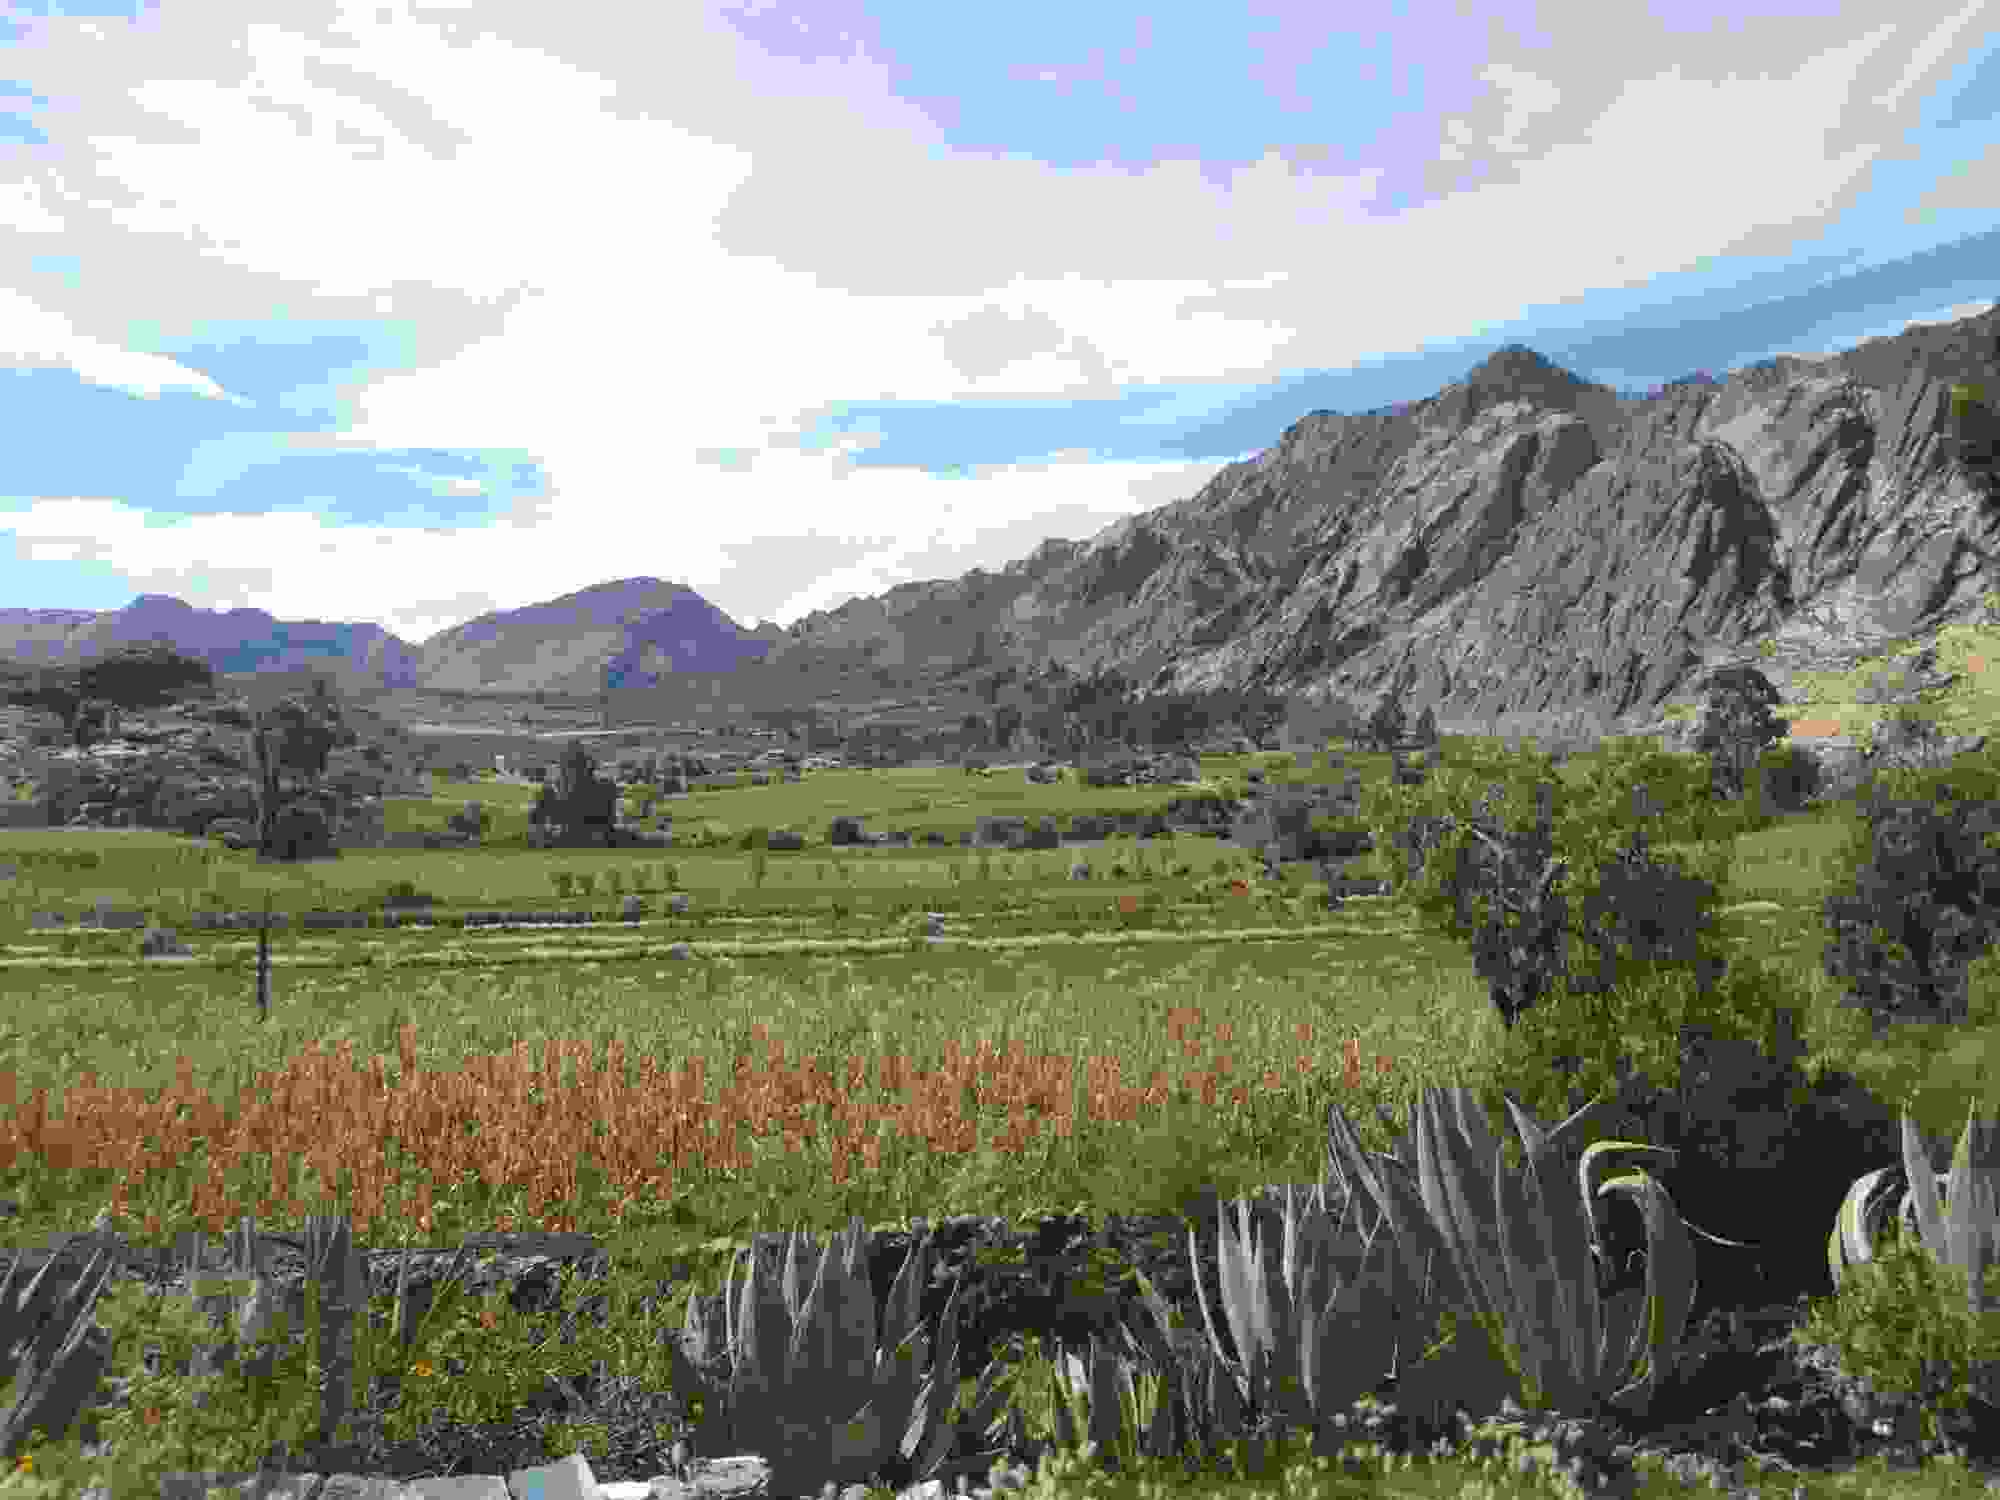
\includegraphics[width=\mywidth]{../wp-content/uploads/2015/04/wpid-wp-1429062375616.jpg} \end{center}
\begin{center} 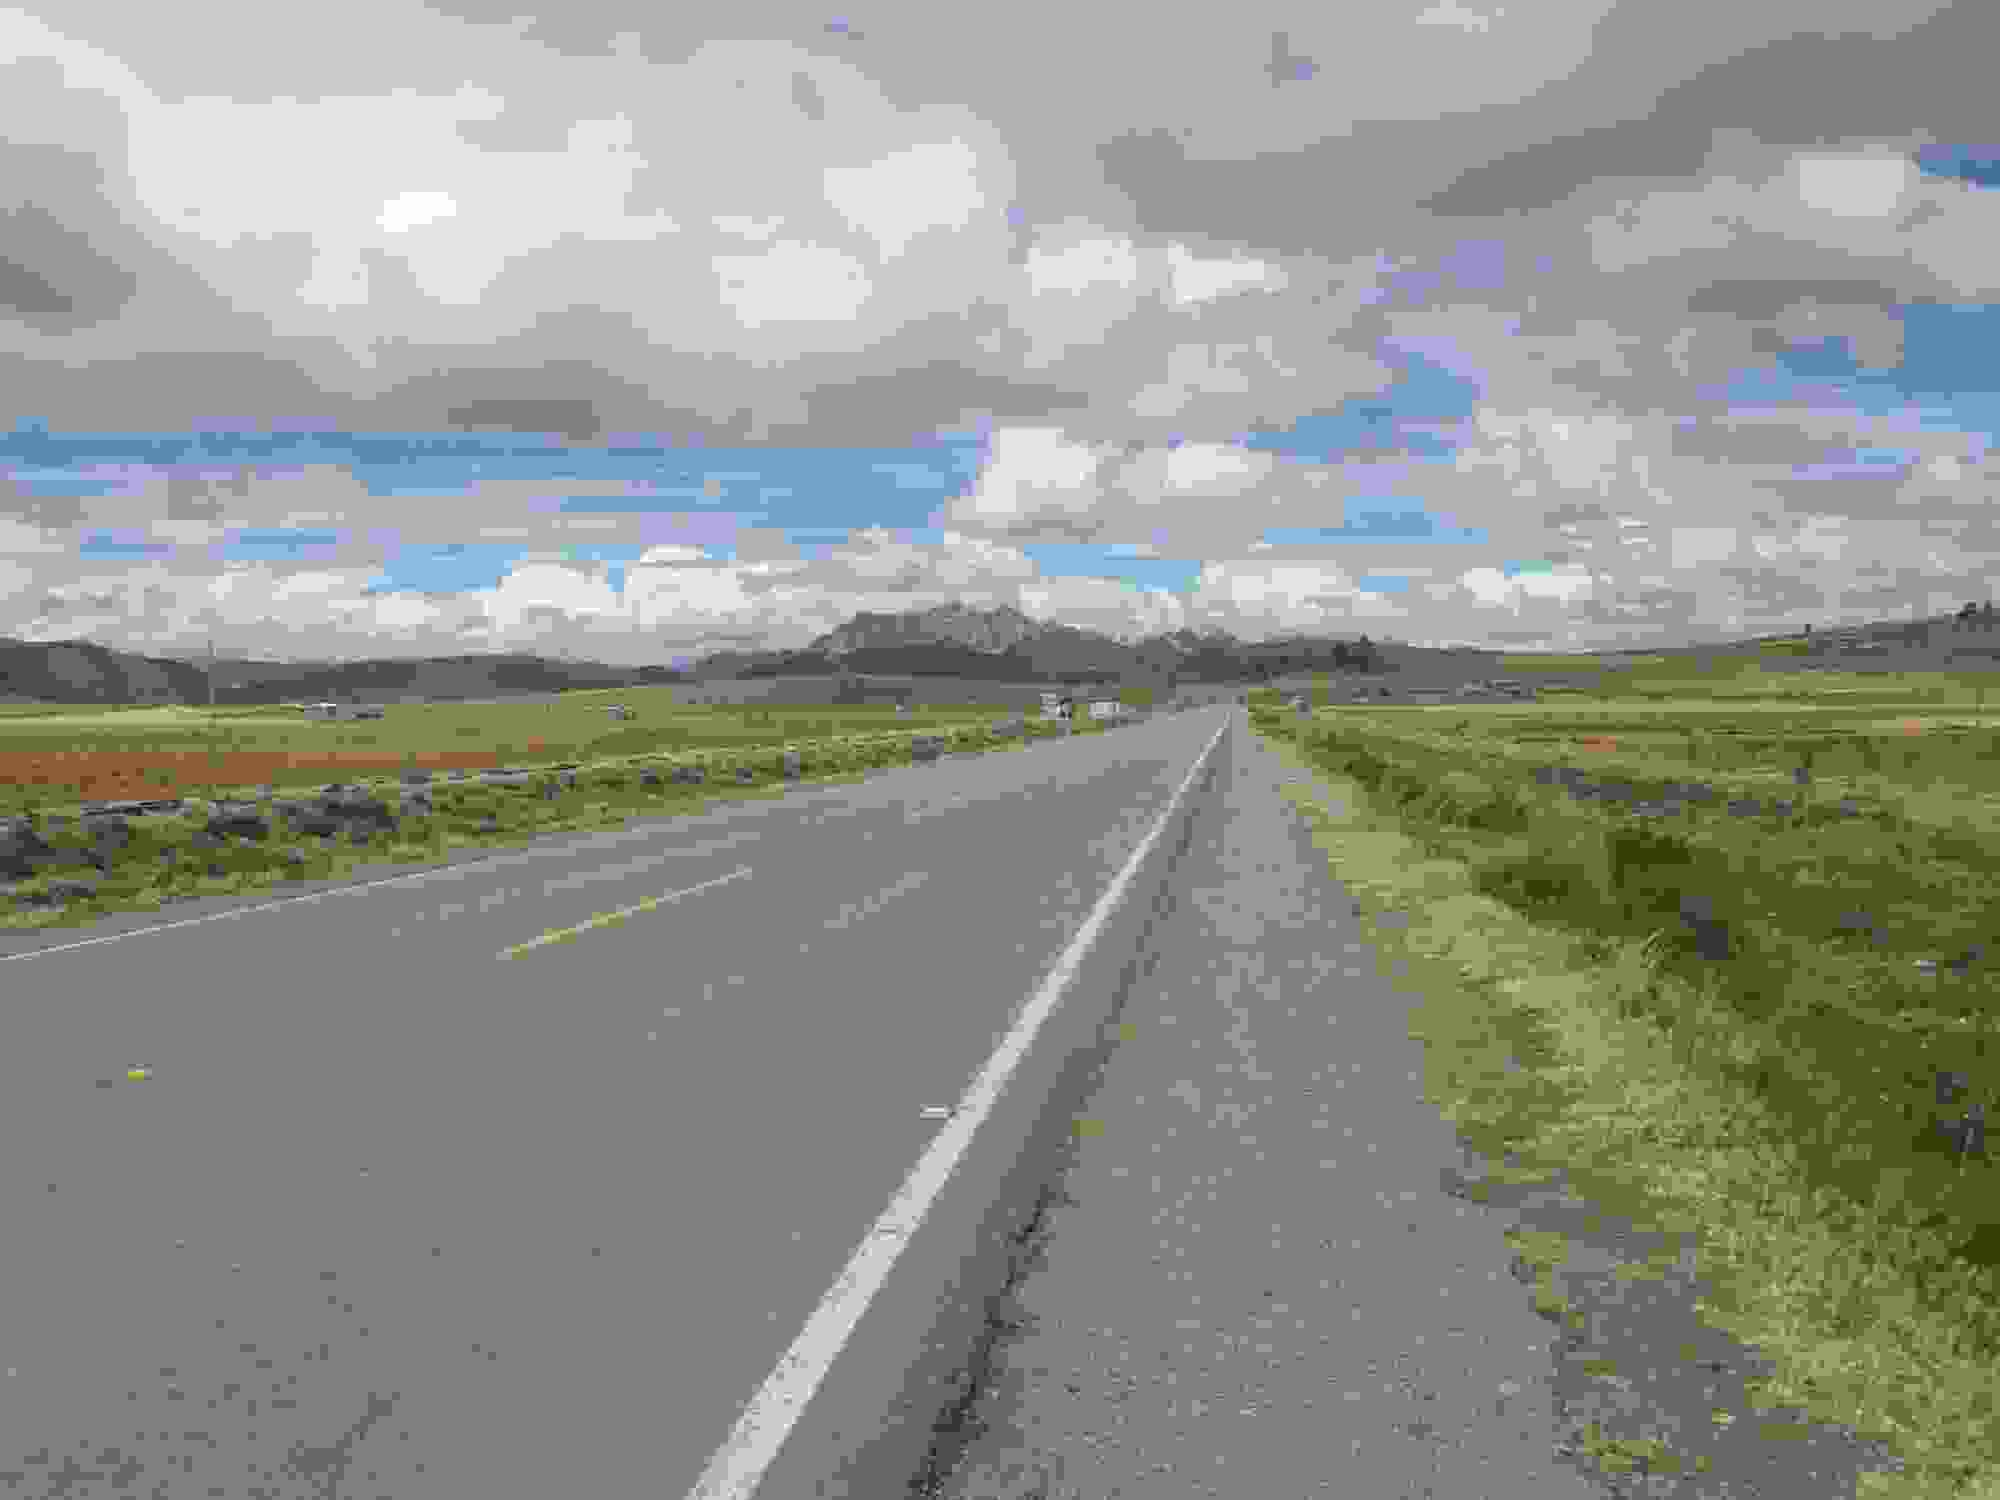
\includegraphics[width=\mywidth]{../wp-content/uploads/2015/04/wpid-wp-1429062400183.jpg} \end{center}

 Les lamas sont progressivement remplacés par les vaches et les moutons. Beaucoup de chiens aussi dont quelques uns un peu agressifs.

 Toujours de beaux paysages sur la route. 
\begin{center} 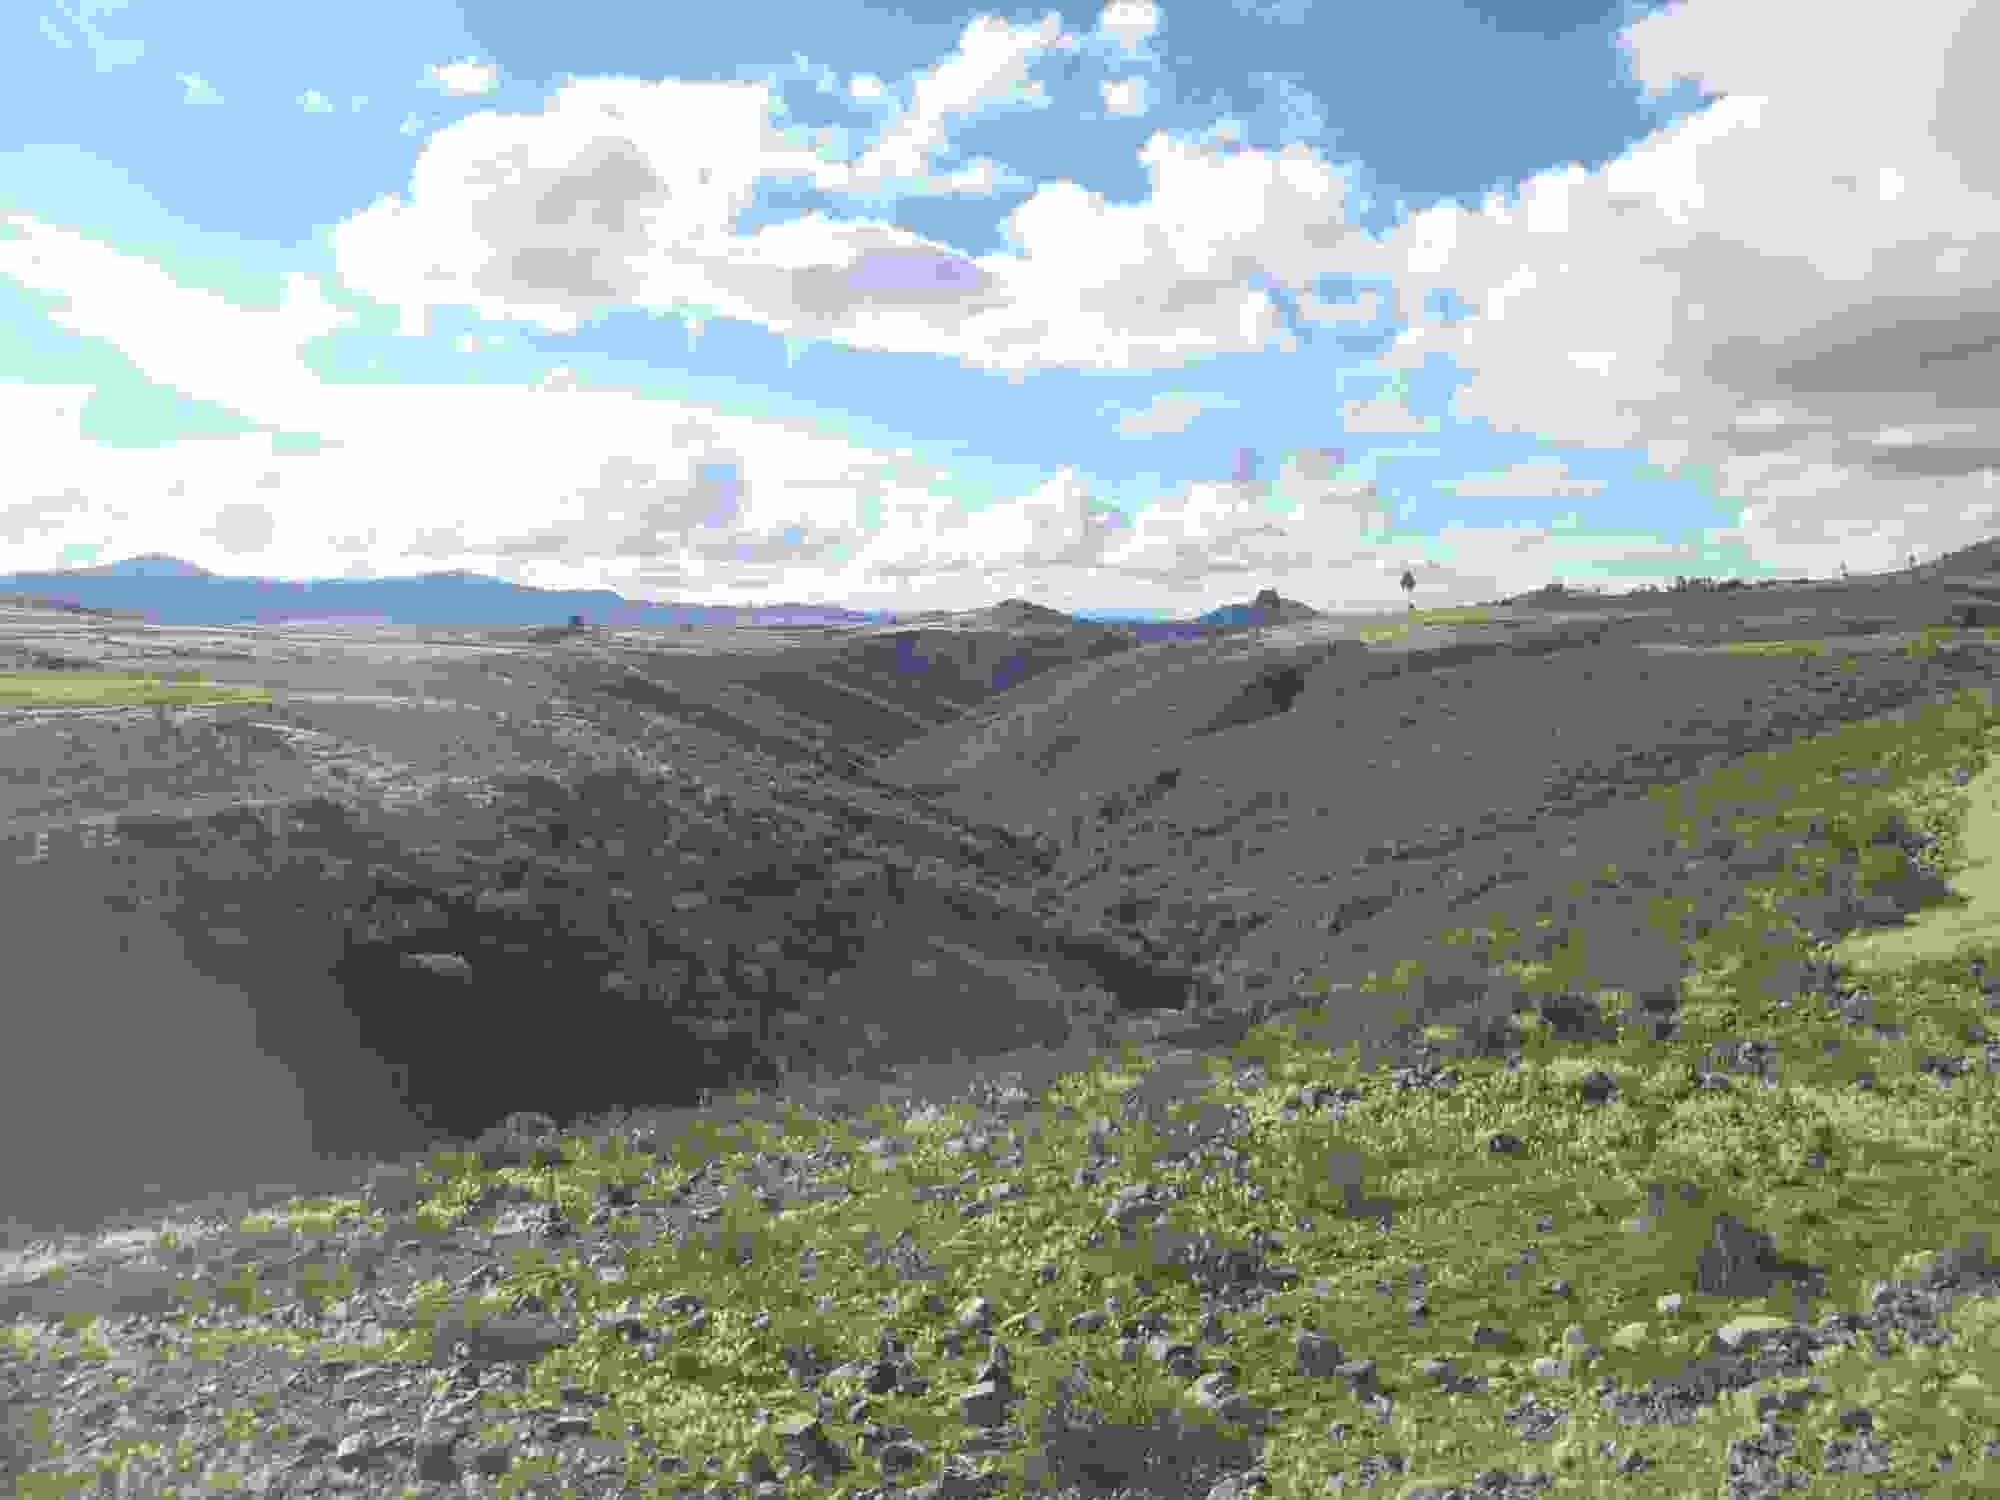
\includegraphics[width=\mywidth]{../wp-content/uploads/2015/04/wpid-wp-1429062516923.jpg} \end{center}
\begin{center} 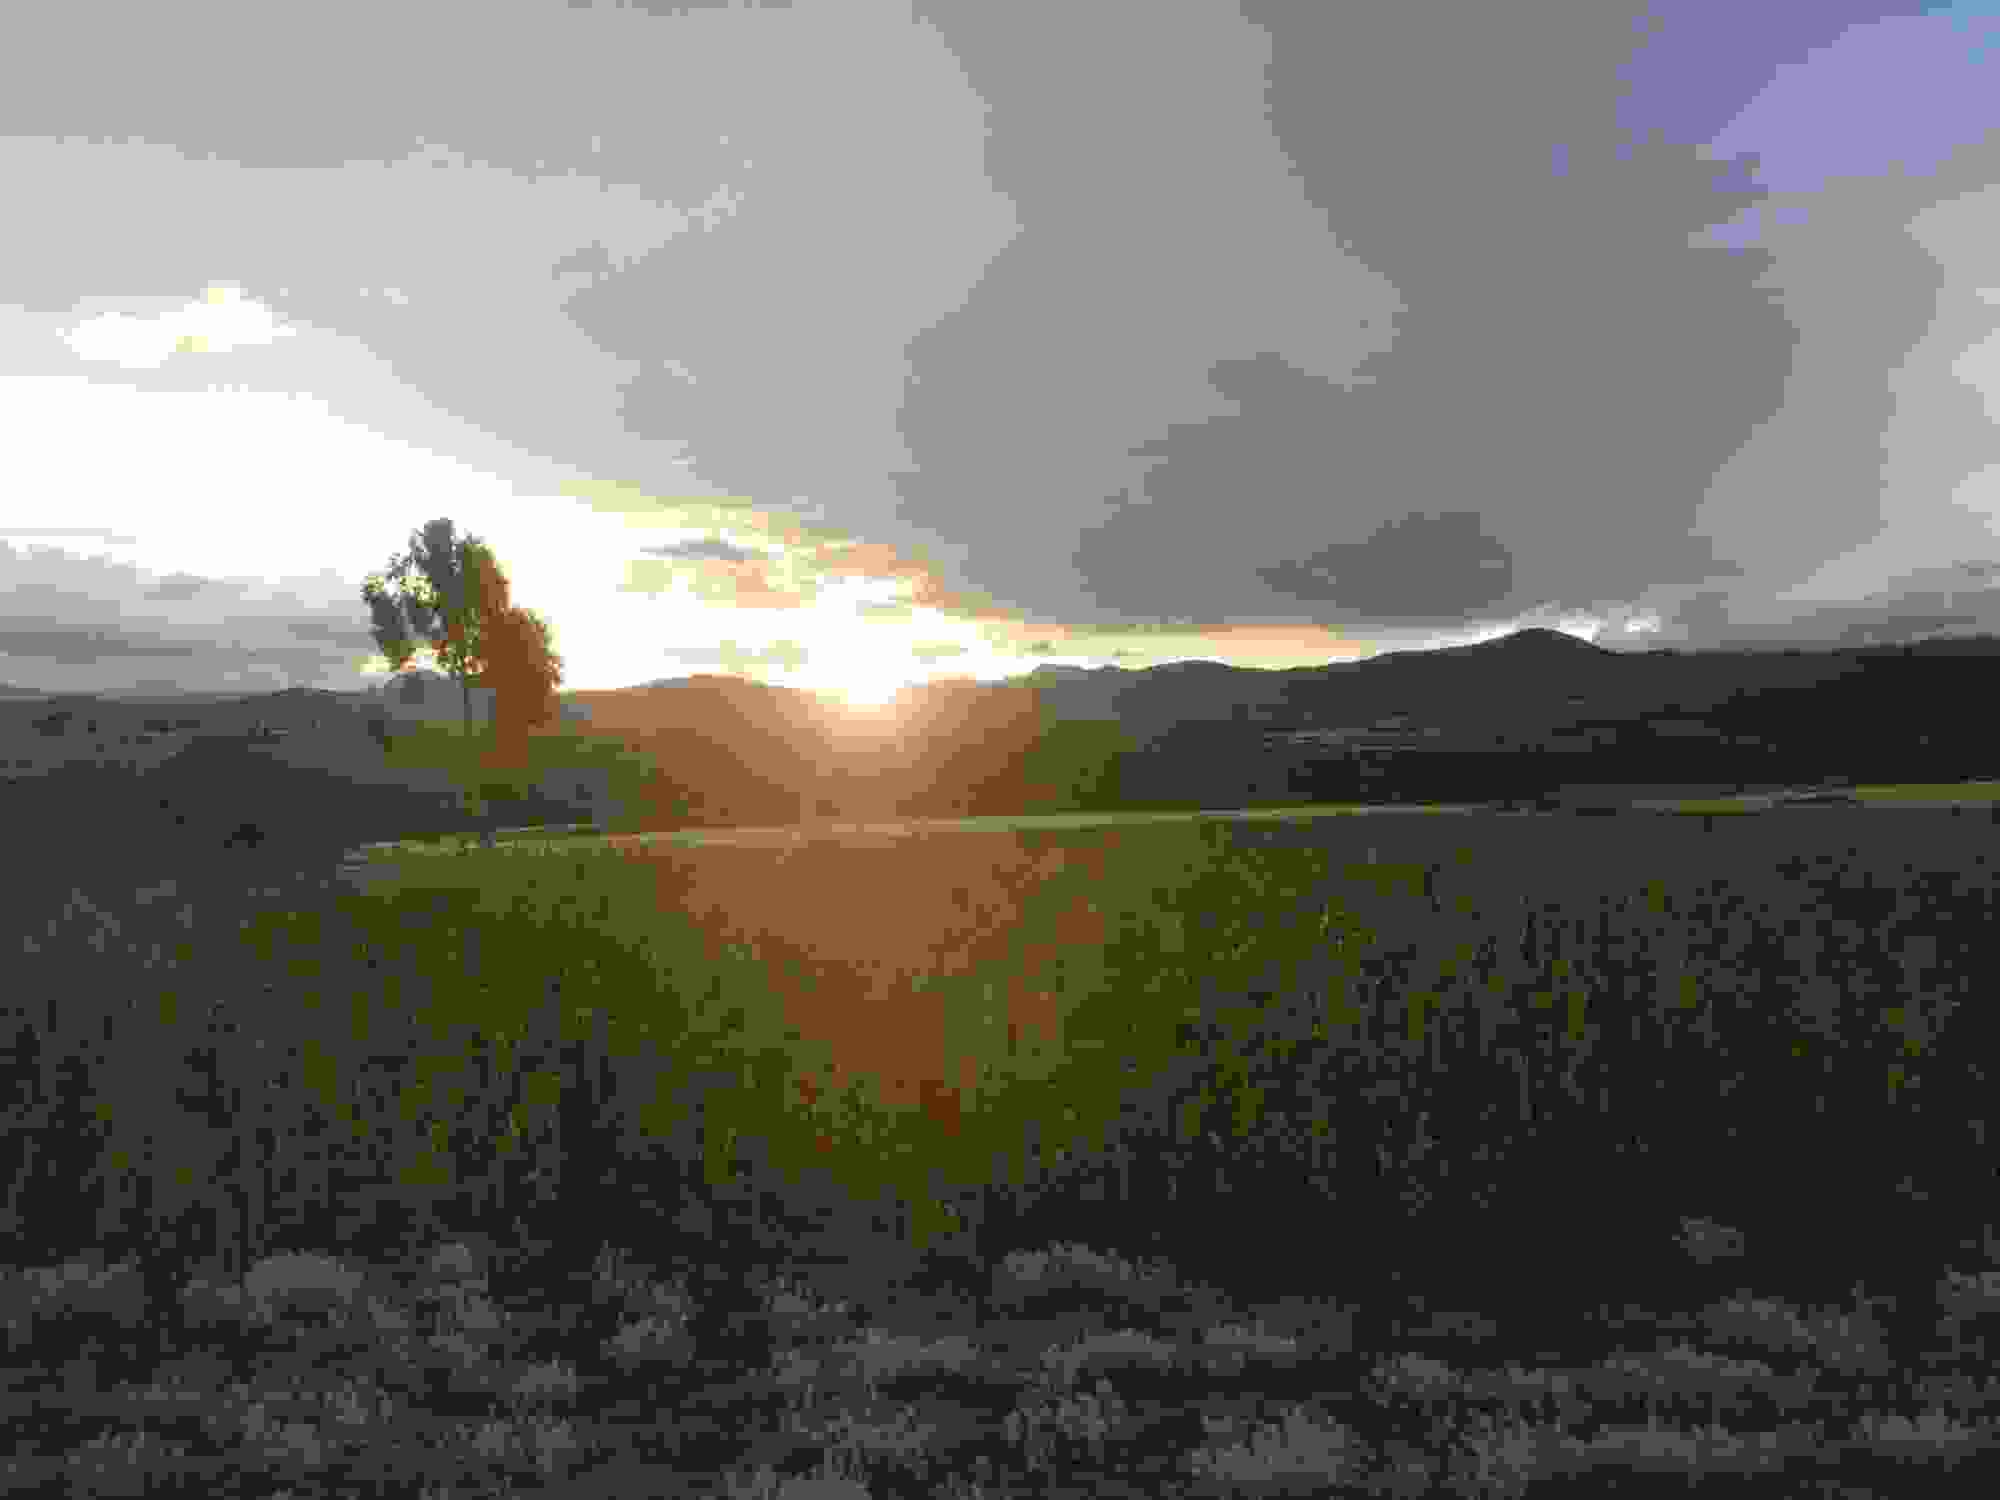
\includegraphics[width=\mywidth]{../wp-content/uploads/2015/04/wpid-wp-1429062575398.jpg} \end{center}
\vfill
\begin{center} 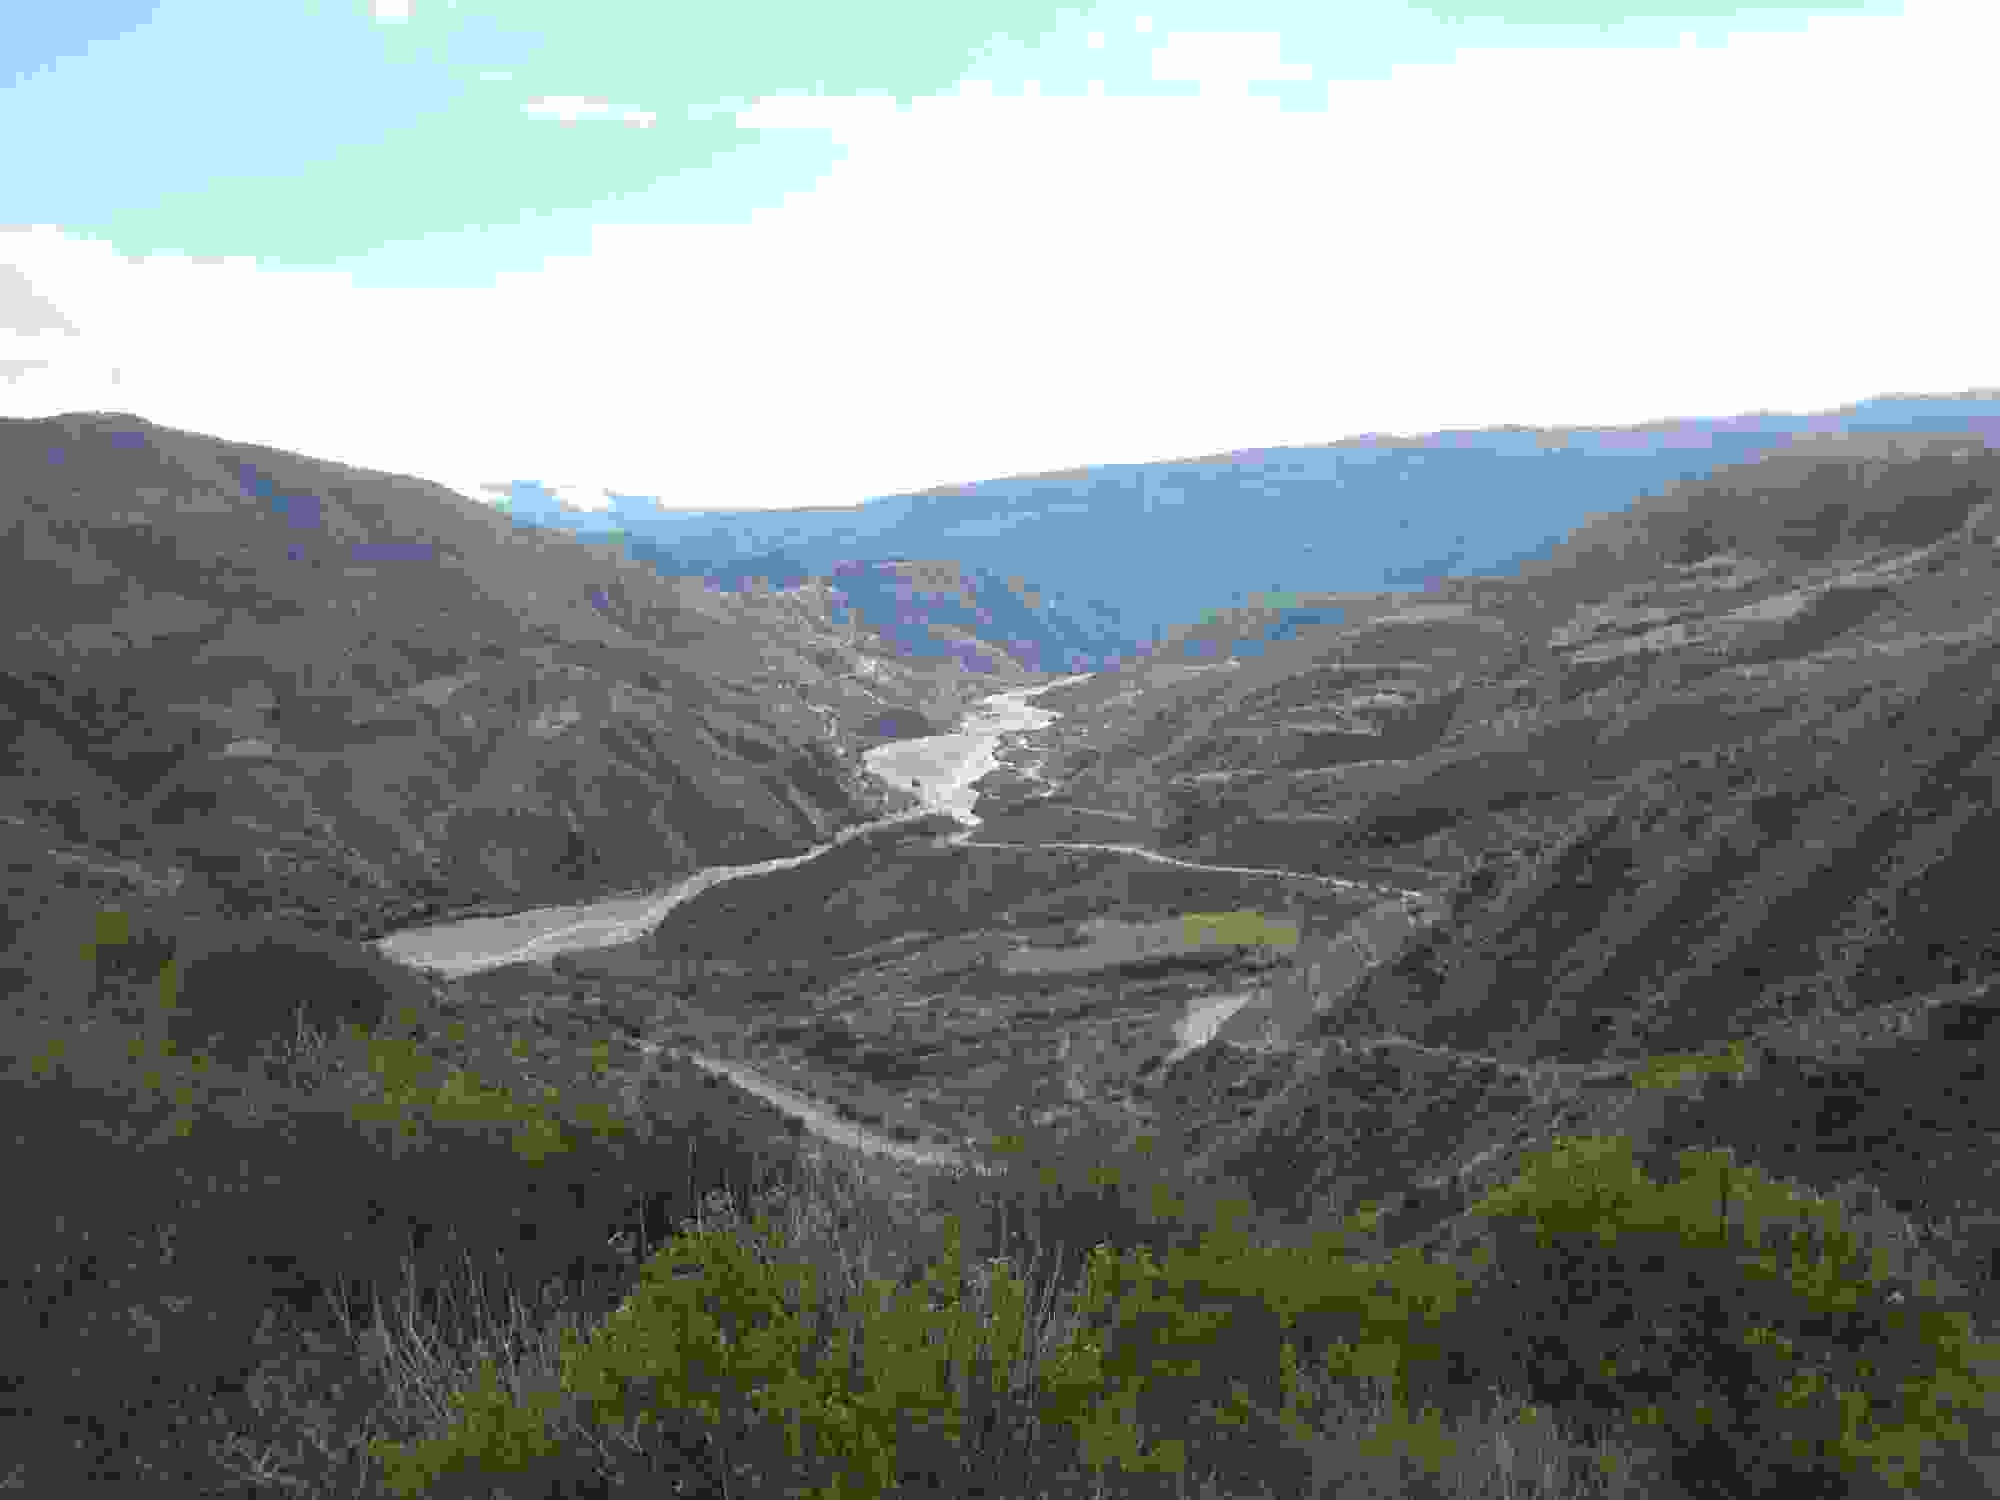
\includegraphics[width=\mywidth]{../wp-content/uploads/2015/04/wpid-wp-1429062588750.jpg} \end{center}
\vspace{-\topsep}
\vspace{-0.75mm}

\pagebreak
 En 2 jours j'arrive à Sucre, la capitale judiciaire du pays.

 La ville contraste énormément avec ce que j'ai vu de la Bolivie jusqu'à présent : très agréable, plutôt propre et avec un climat doux. Même les gens semblent plus souriants. 
\begin{center} 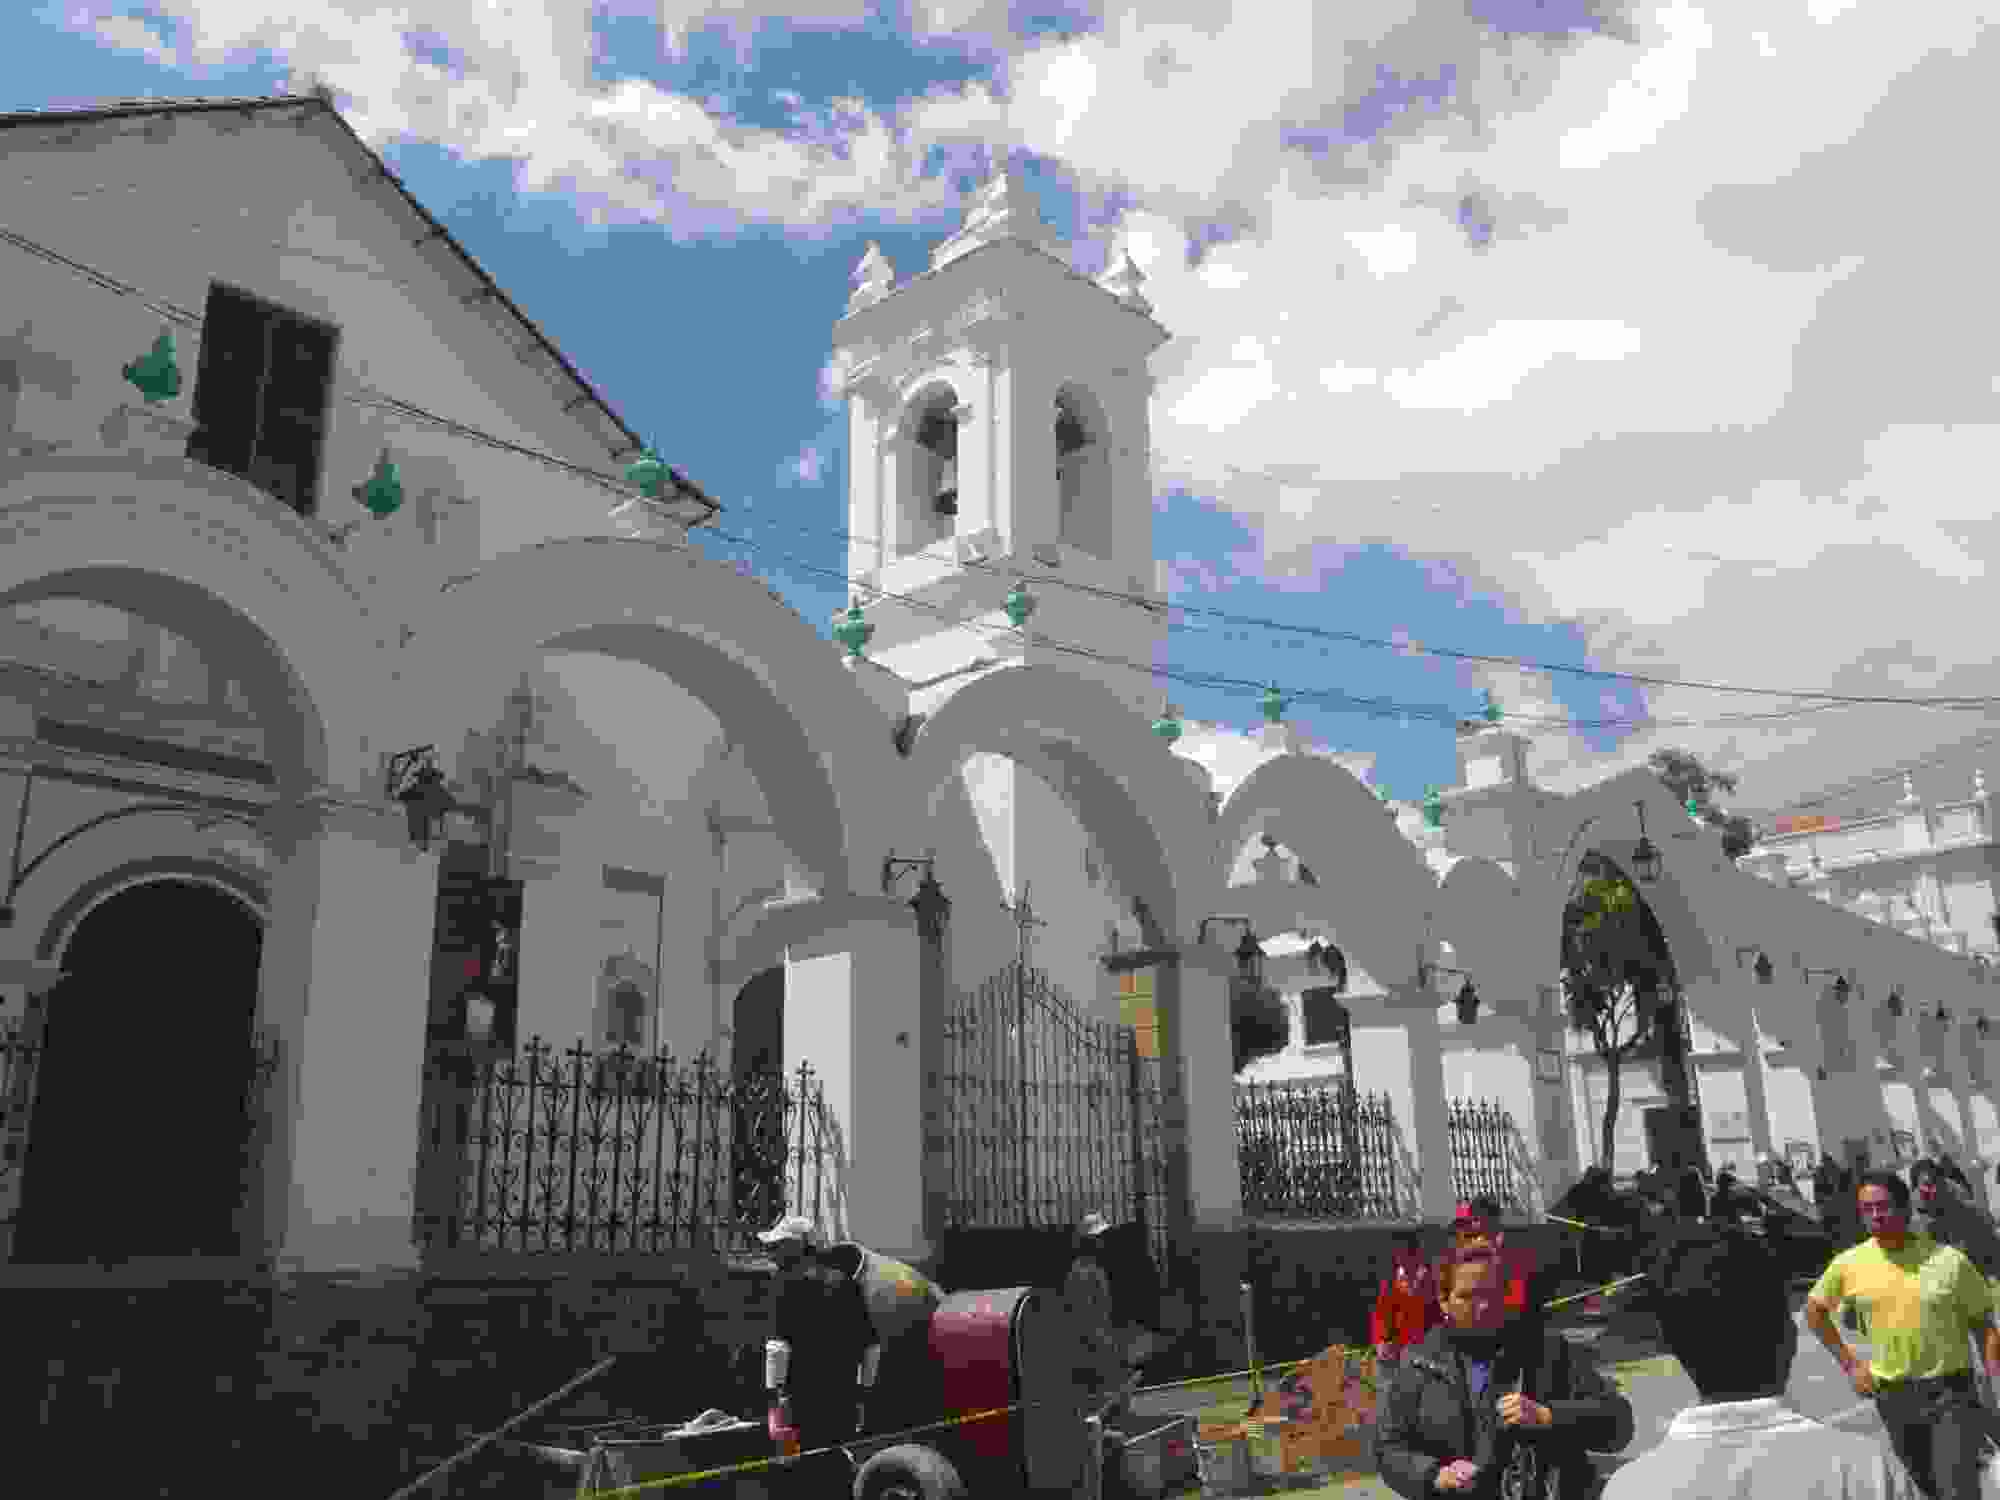
\includegraphics[width=\mywidth]{../wp-content/uploads/2015/04/wpid-wp-1429063237665.jpg} \end{center}
\begin{center} 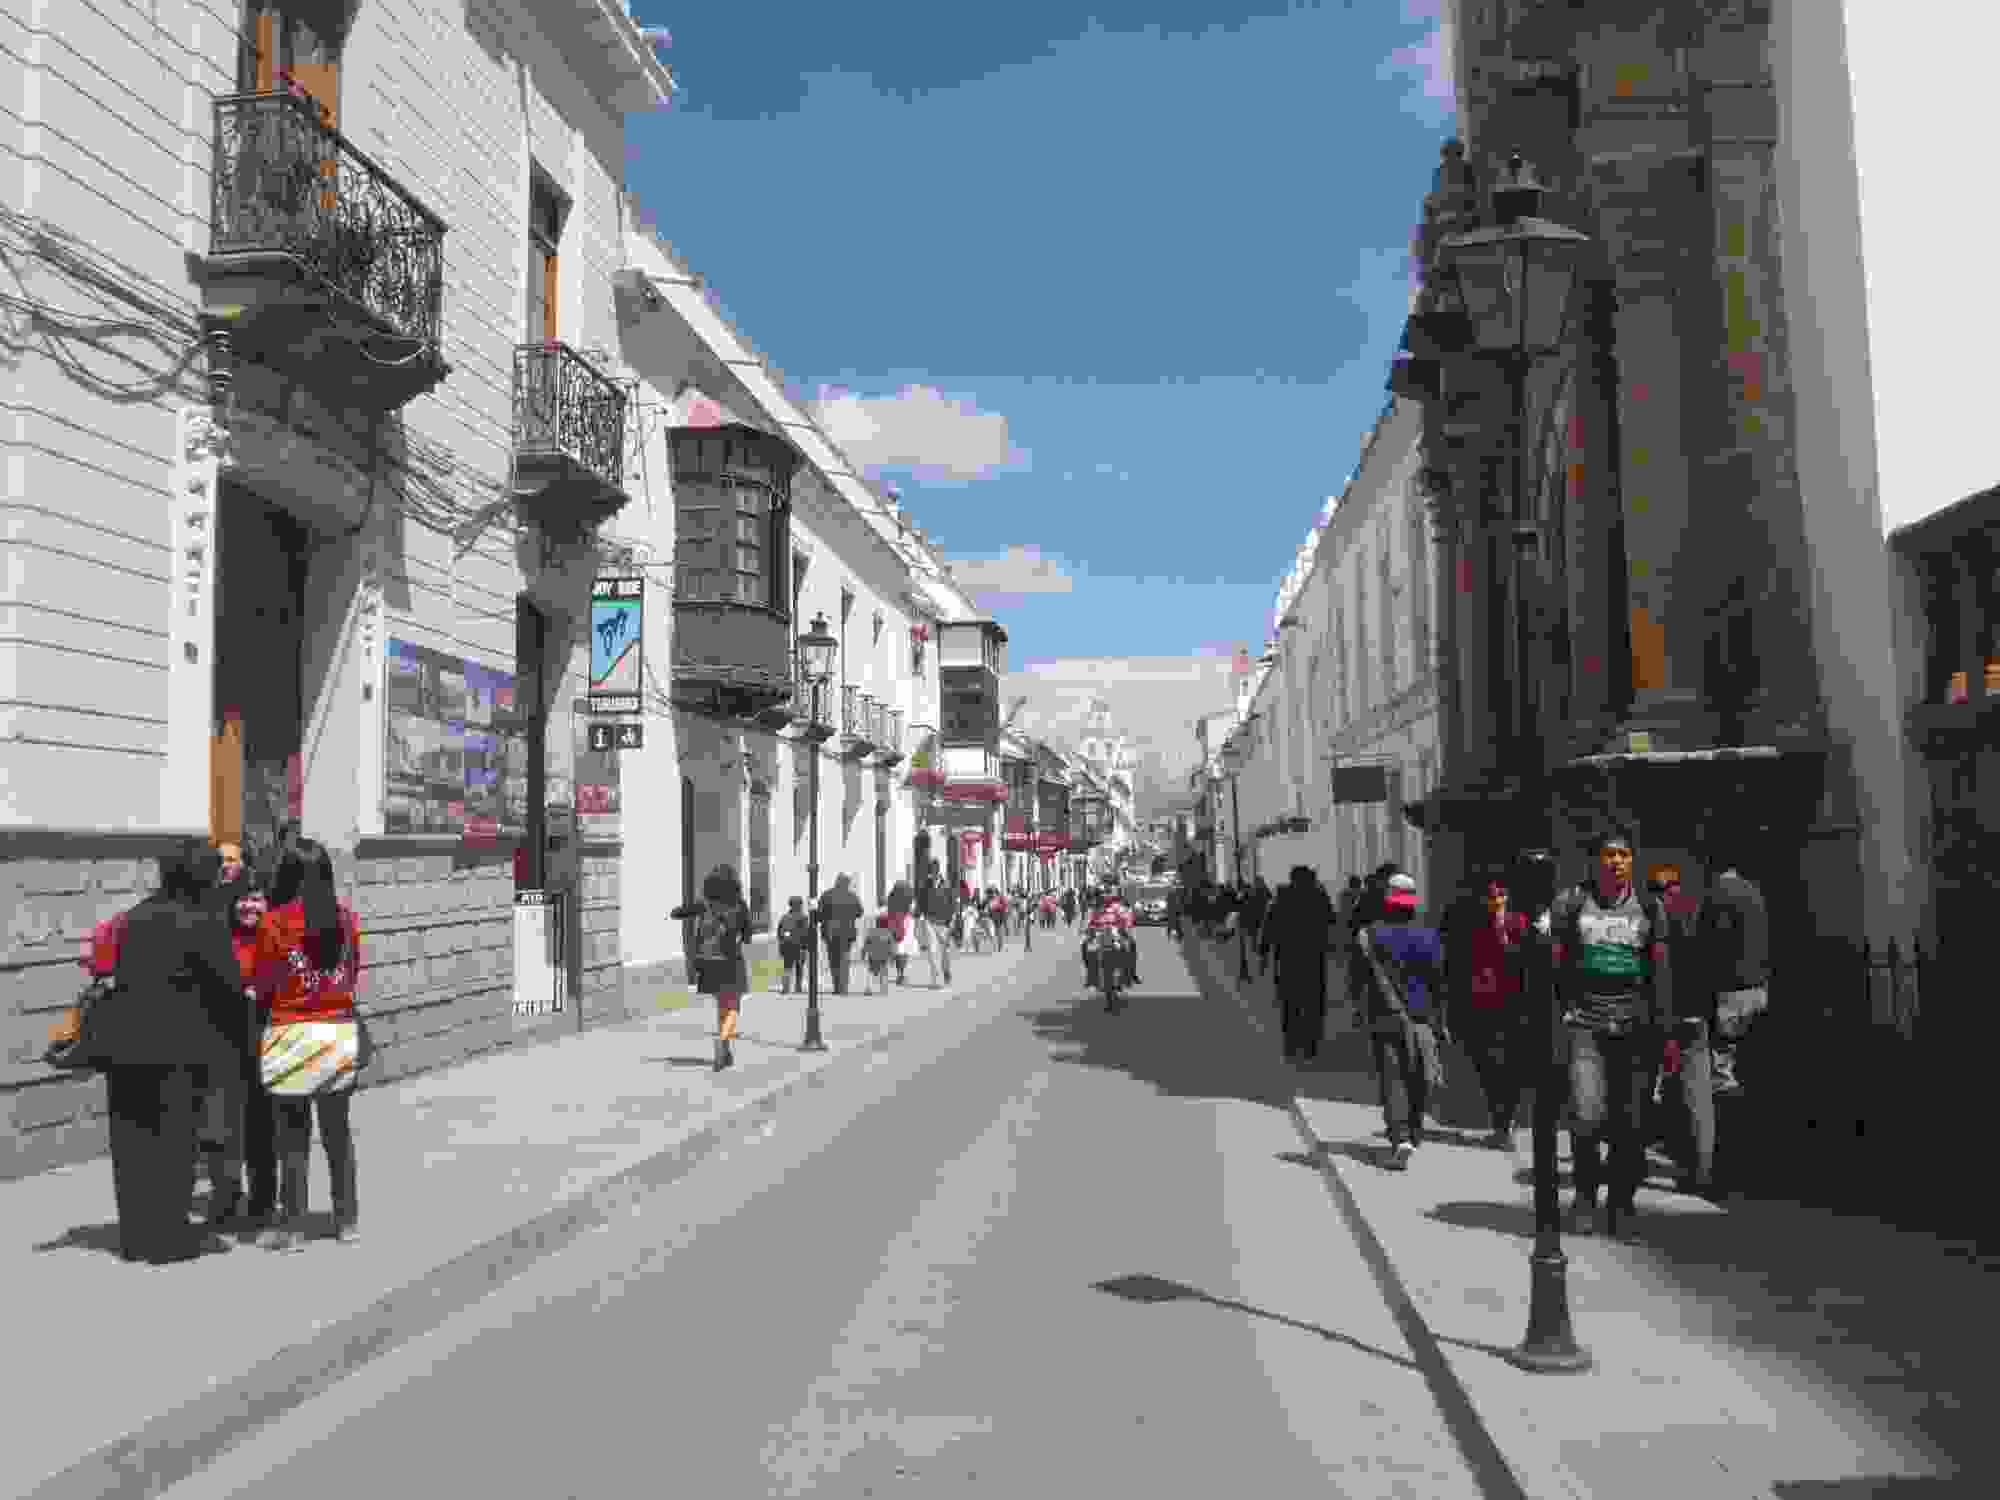
\includegraphics[width=\mywidth]{../wp-content/uploads/2015/04/wpid-wp-1429063251282.jpg} \end{center}
\vspace{-\topsep}
\vspace{-1.75mm}

\pagebreak
 La Plaza 25 de Mayo.
 
 ~\\~\\
 \vspace{0.5mm}
\begin{center} 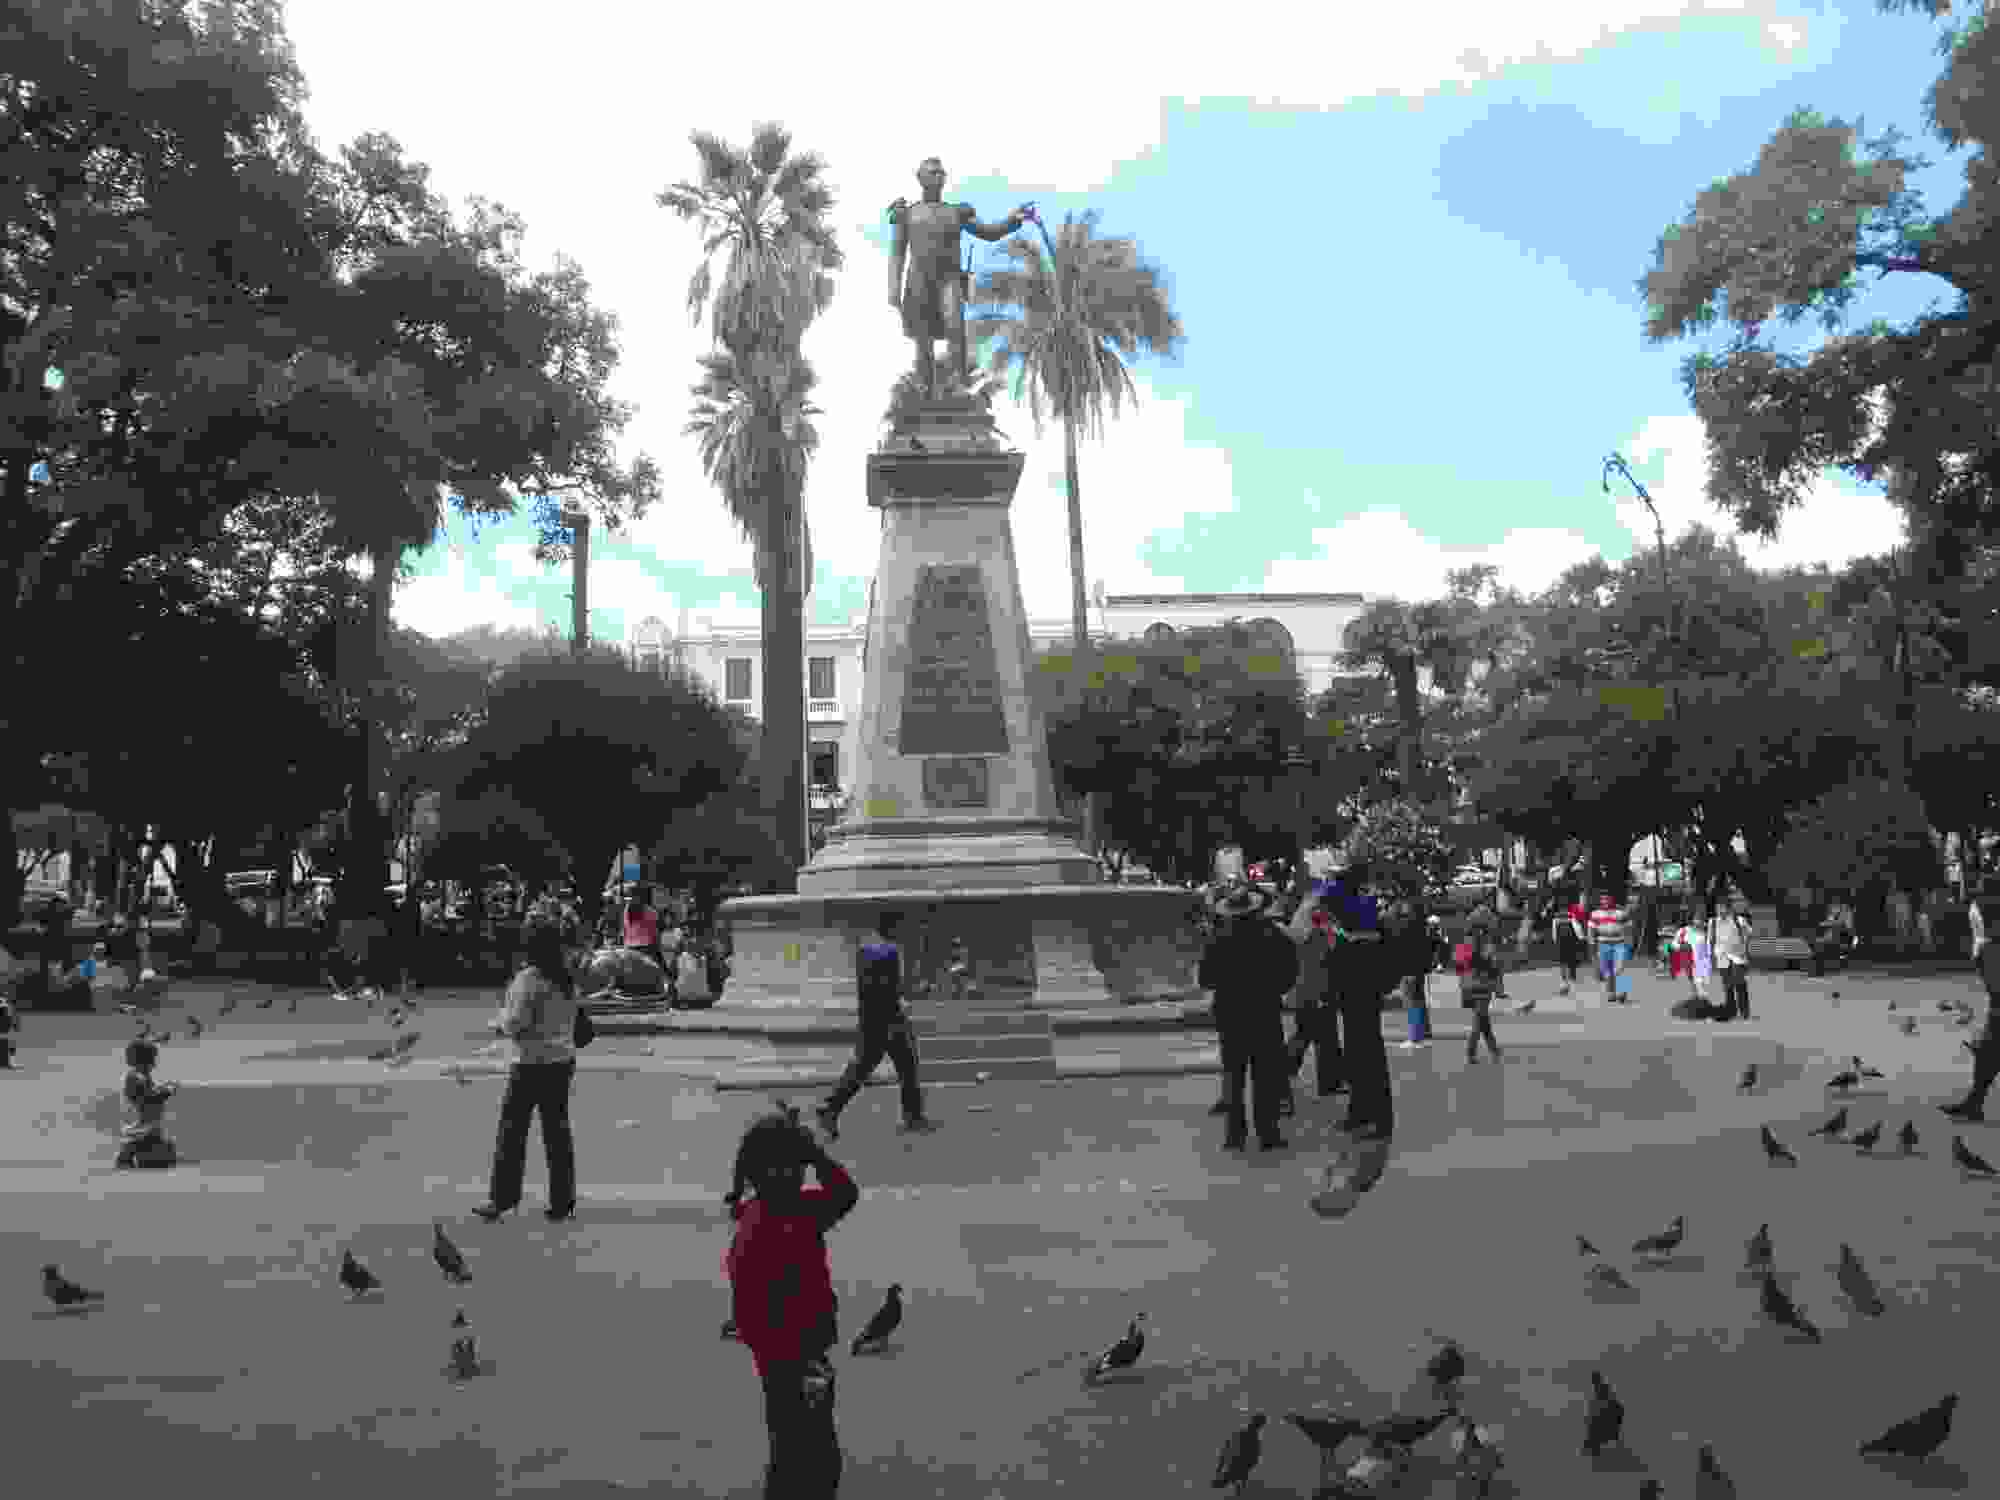
\includegraphics[width=\mywidth]{../wp-content/uploads/2015/04/wpid-wp-1429063361085.jpg} \end{center}
\begin{center} 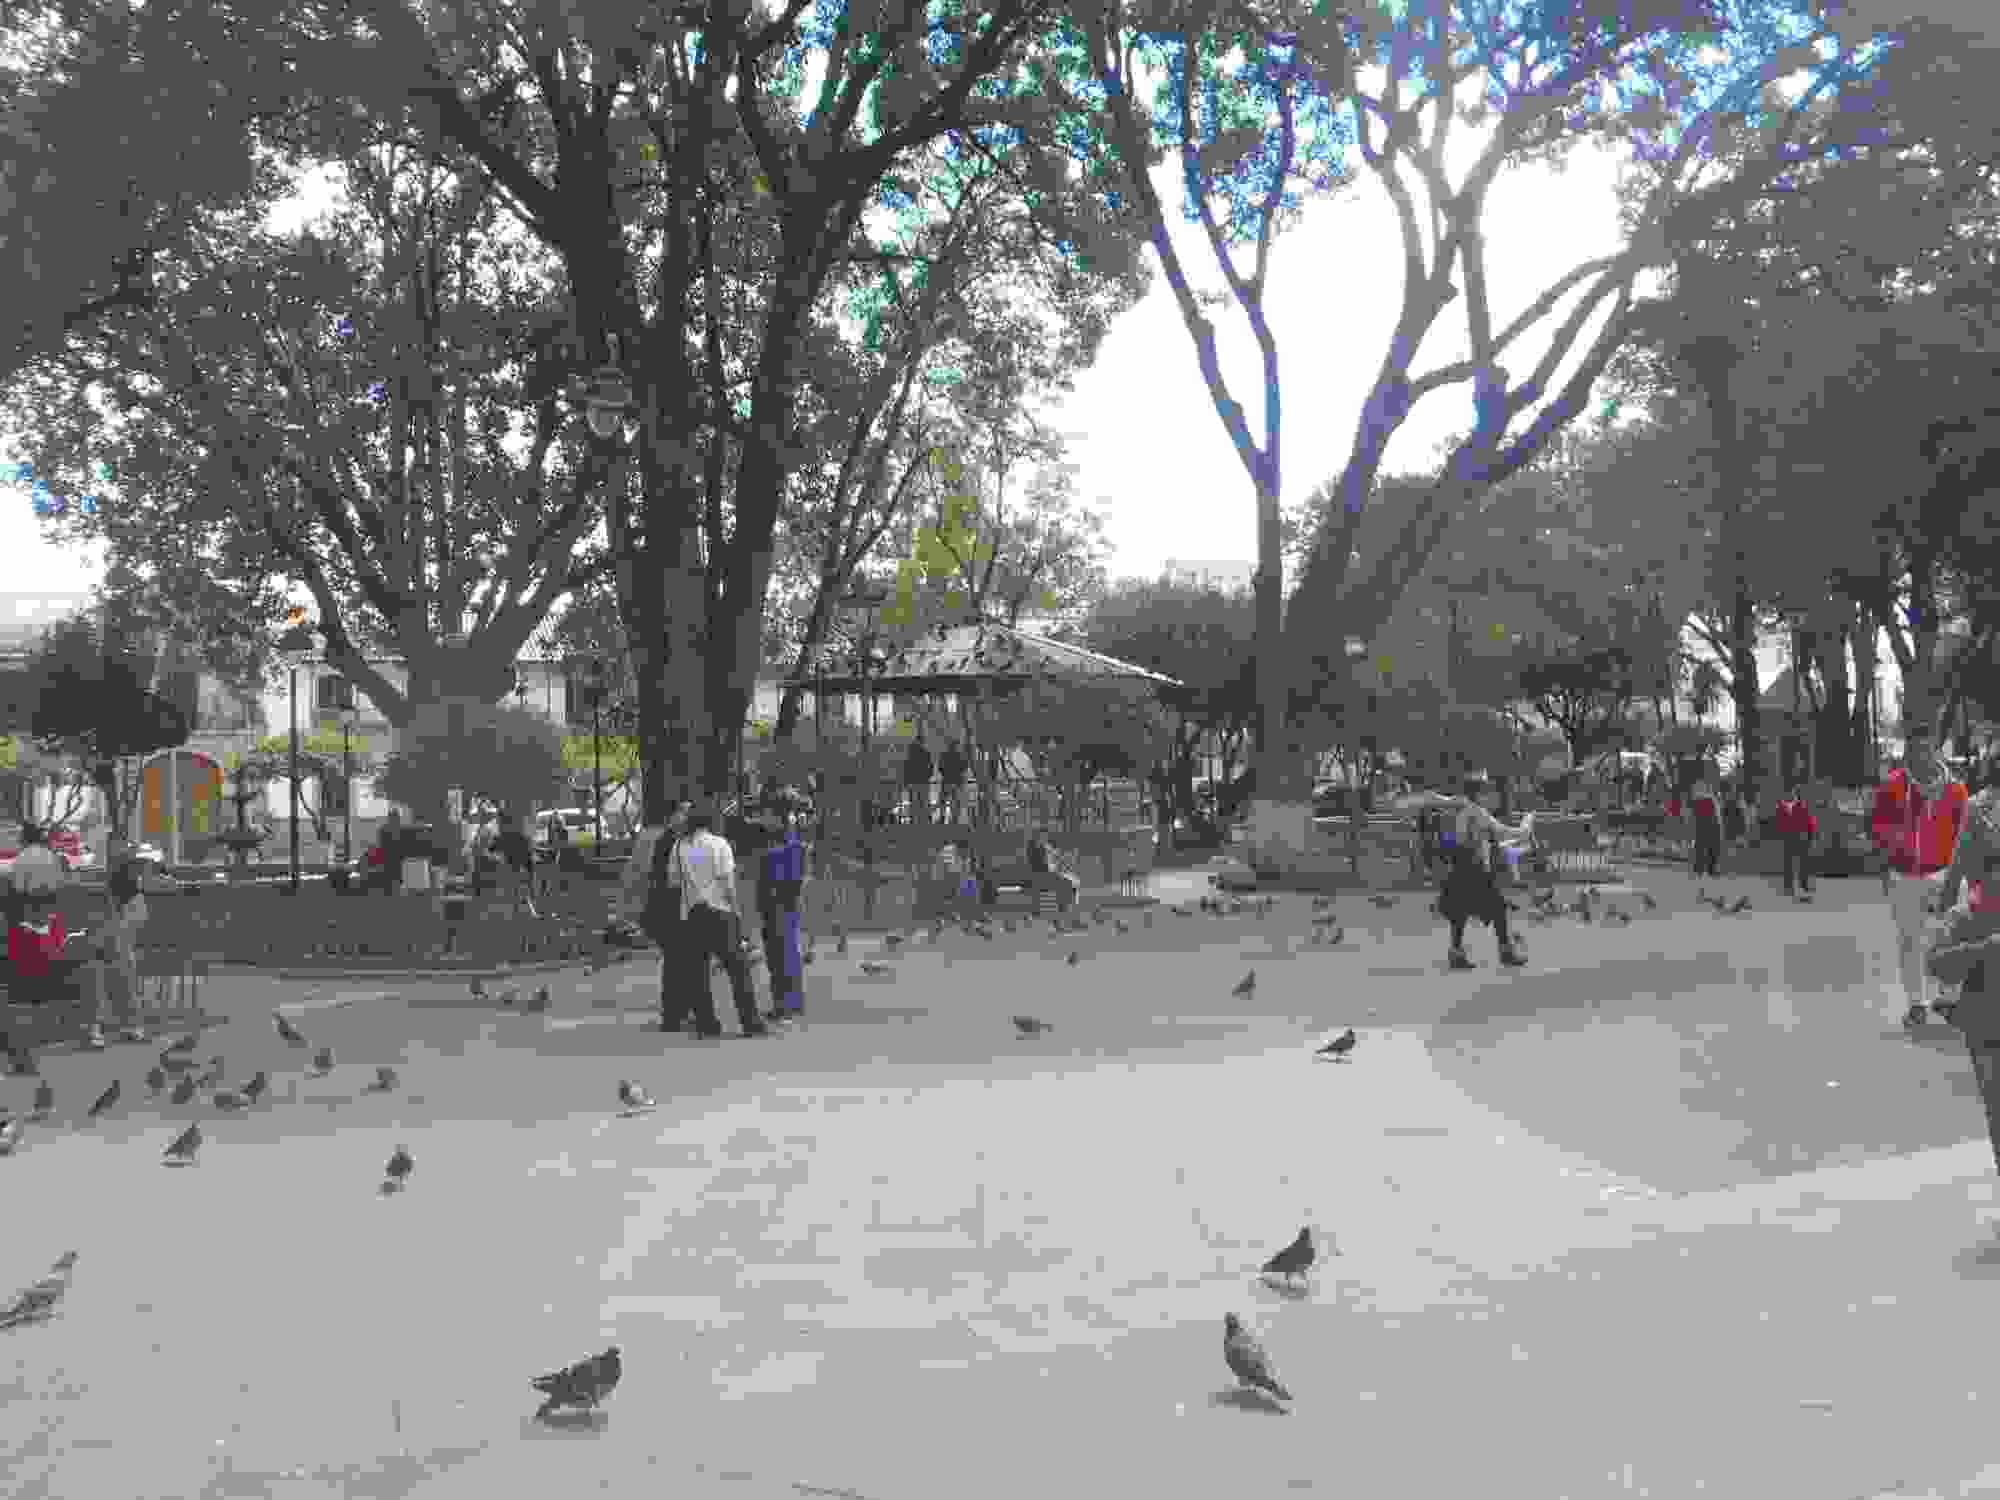
\includegraphics[width=\mywidth]{../wp-content/uploads/2015/04/wpid-wp-1429063375686.jpg} \end{center}
\vspace{-\topsep}
\vspace{-1.75mm}

\pagebreak
 La Casa de la Libertad : la visite explique l'histoire de l'indépendance de la Bolivie avec notamment son premier président Simon Bolivar qui a inspiré le nom du pays. 
\begin{center} 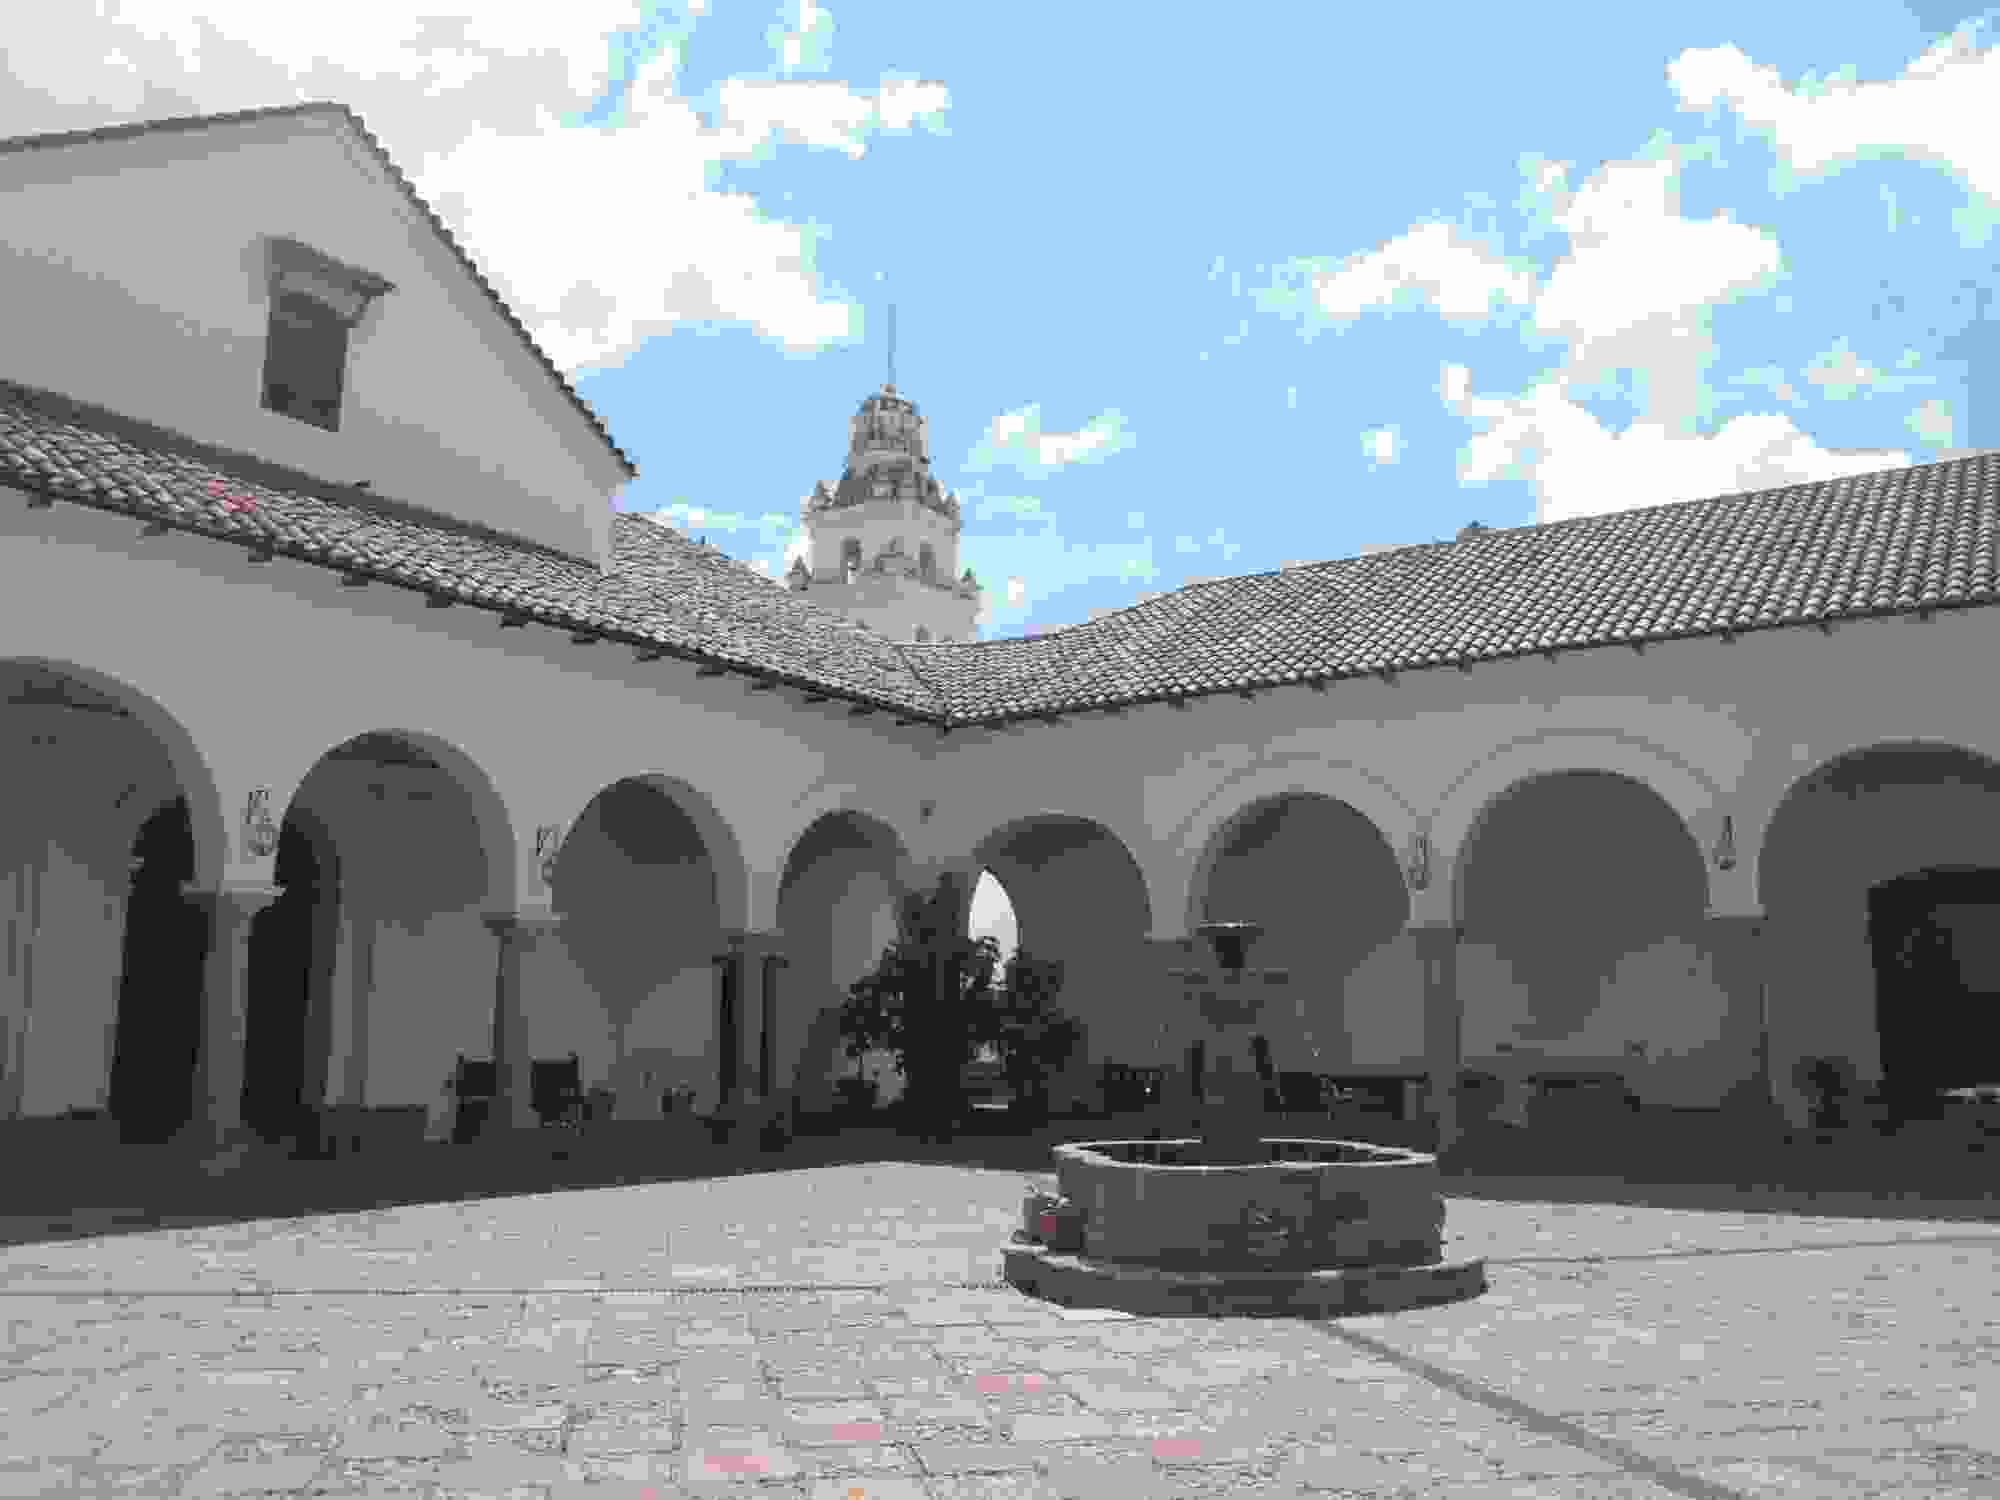
\includegraphics[width=\mywidth]{../wp-content/uploads/2015/04/wpid-wp-1429119927557.jpg} \end{center}
\begin{center} 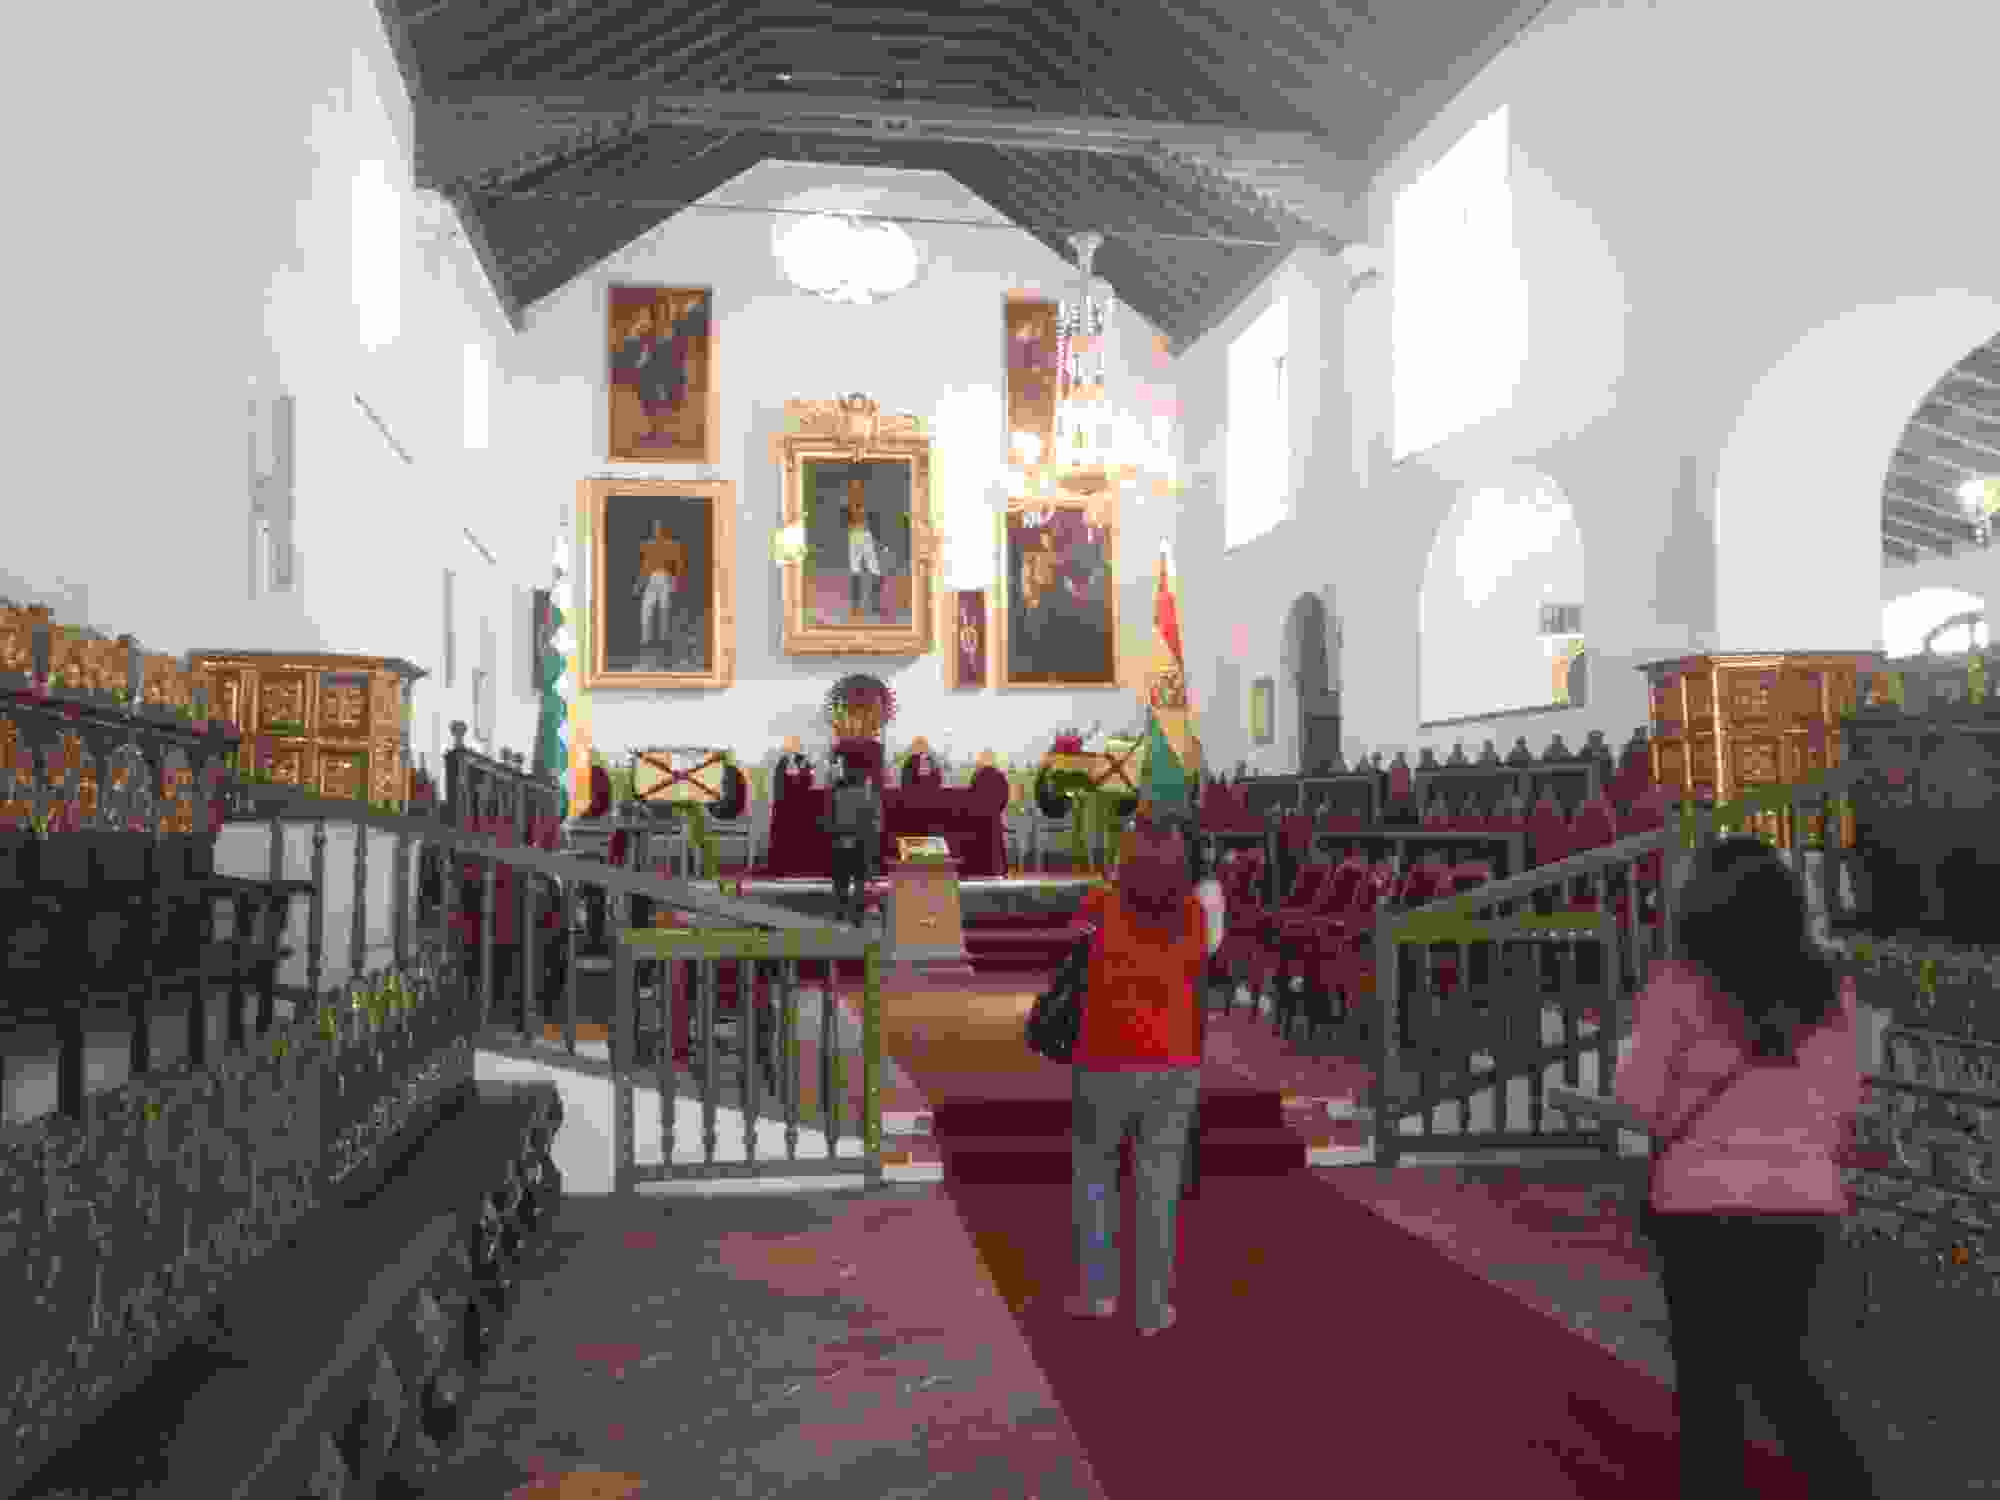
\includegraphics[width=\mywidth]{../wp-content/uploads/2015/04/wpid-wp-1429120135293.jpg} \end{center}
\vspace{-\topsep}
\vspace{-2.25mm}

\pagebreak
 La cathédrale et de belles églises.\\~\\
 \vspace{0.5mm}
\begin{center} 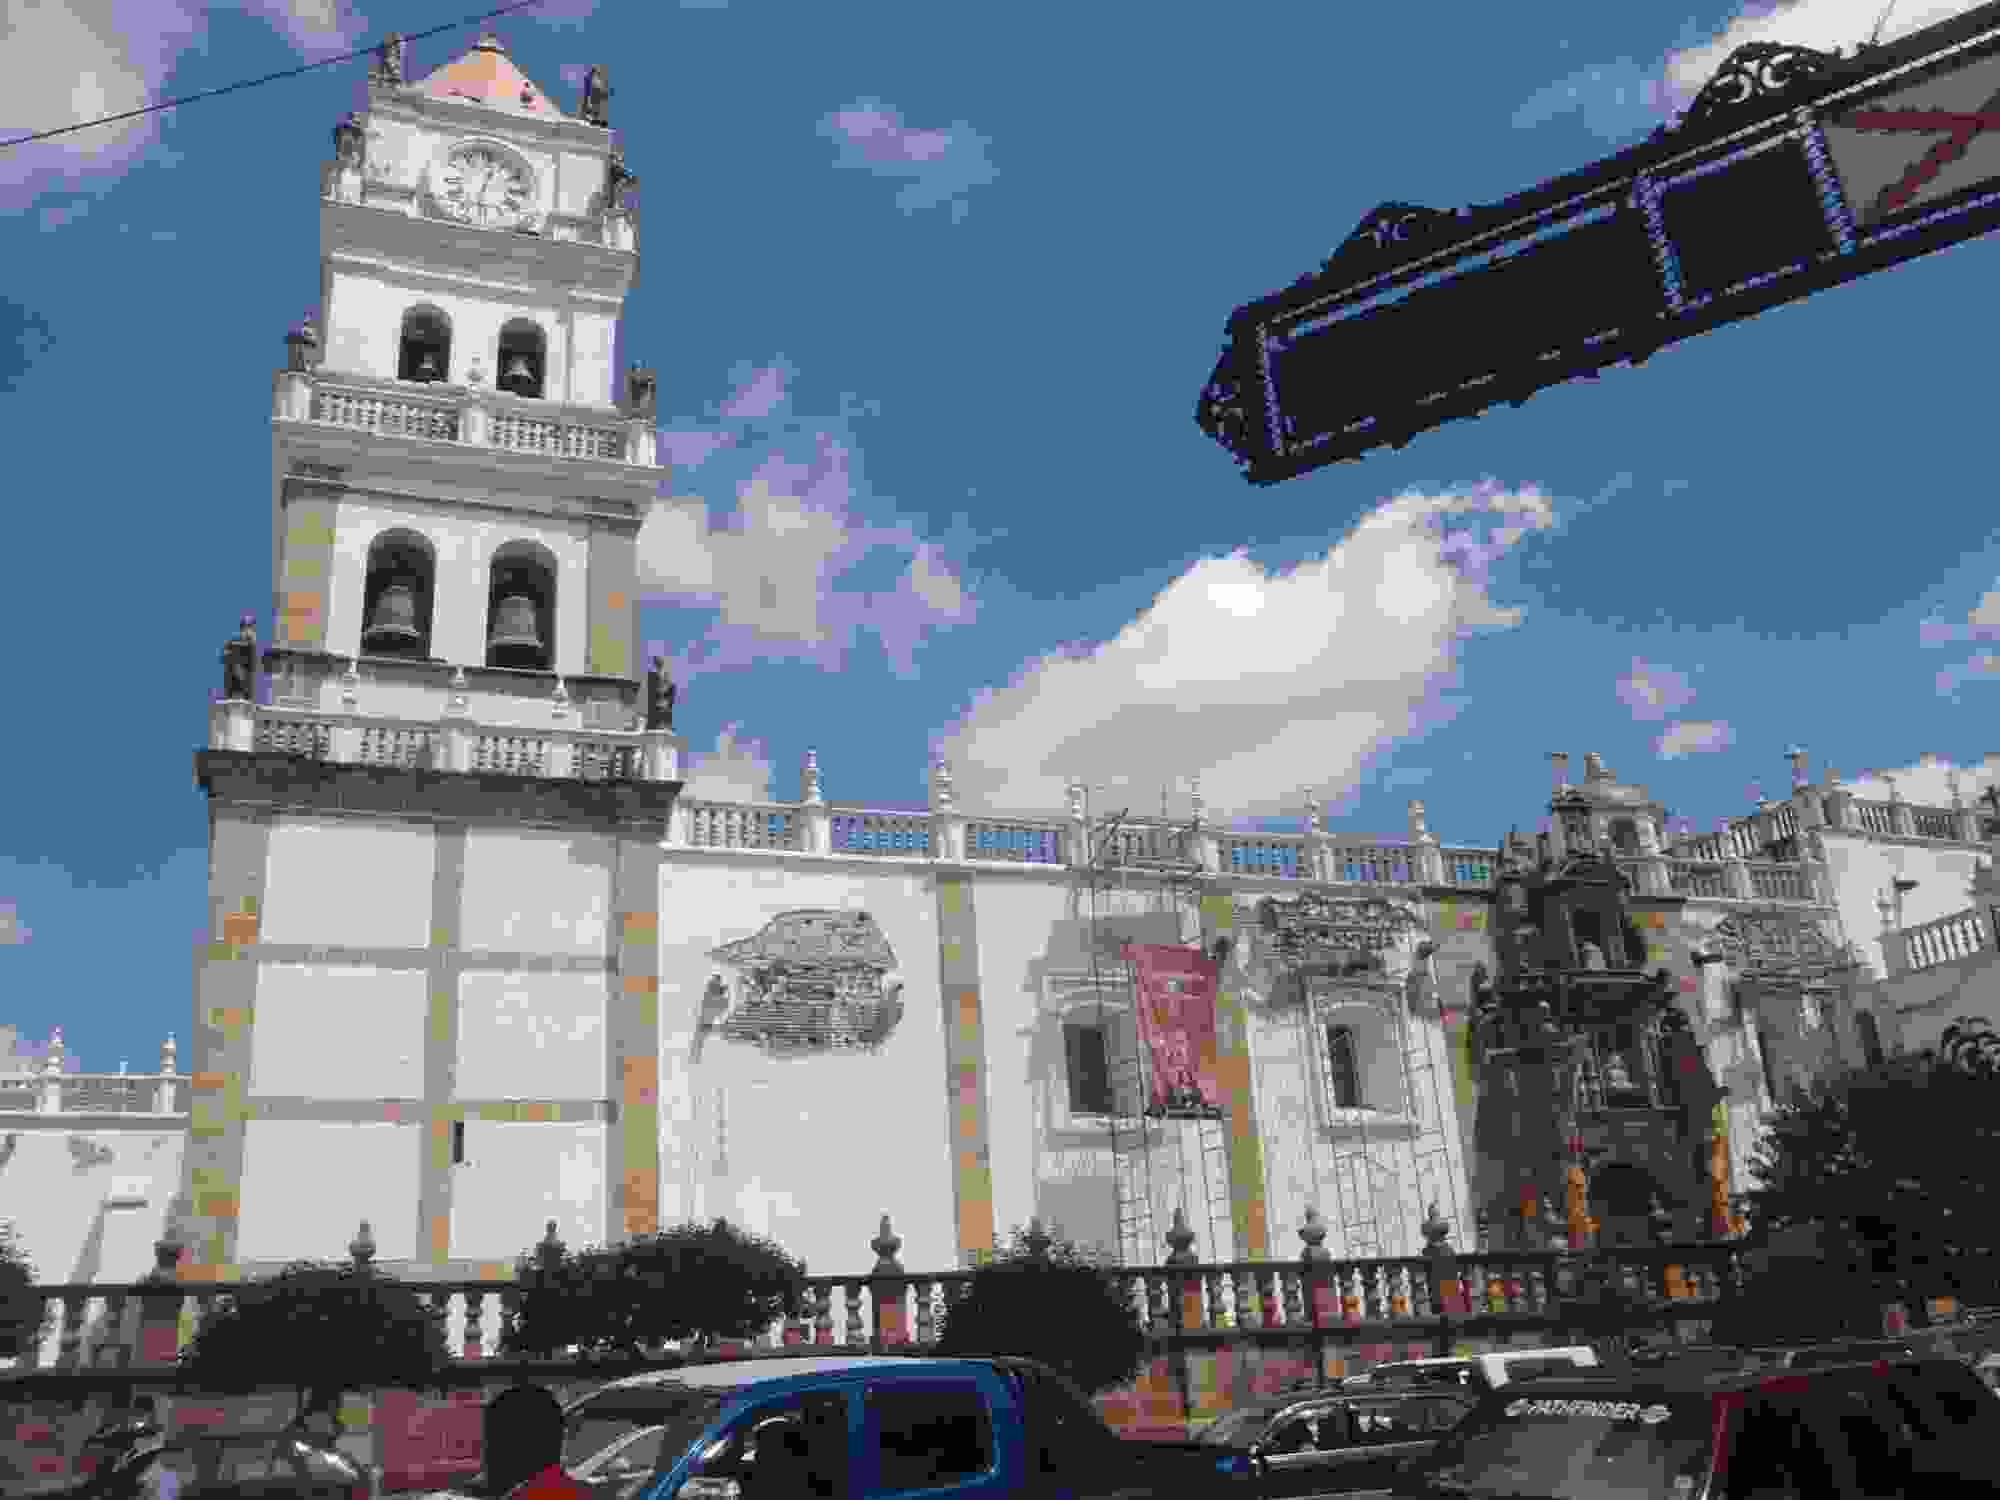
\includegraphics[width=\mywidth]{../wp-content/uploads/2015/04/wpid-wp-1429063401622.jpg} \end{center}
\begin{center} 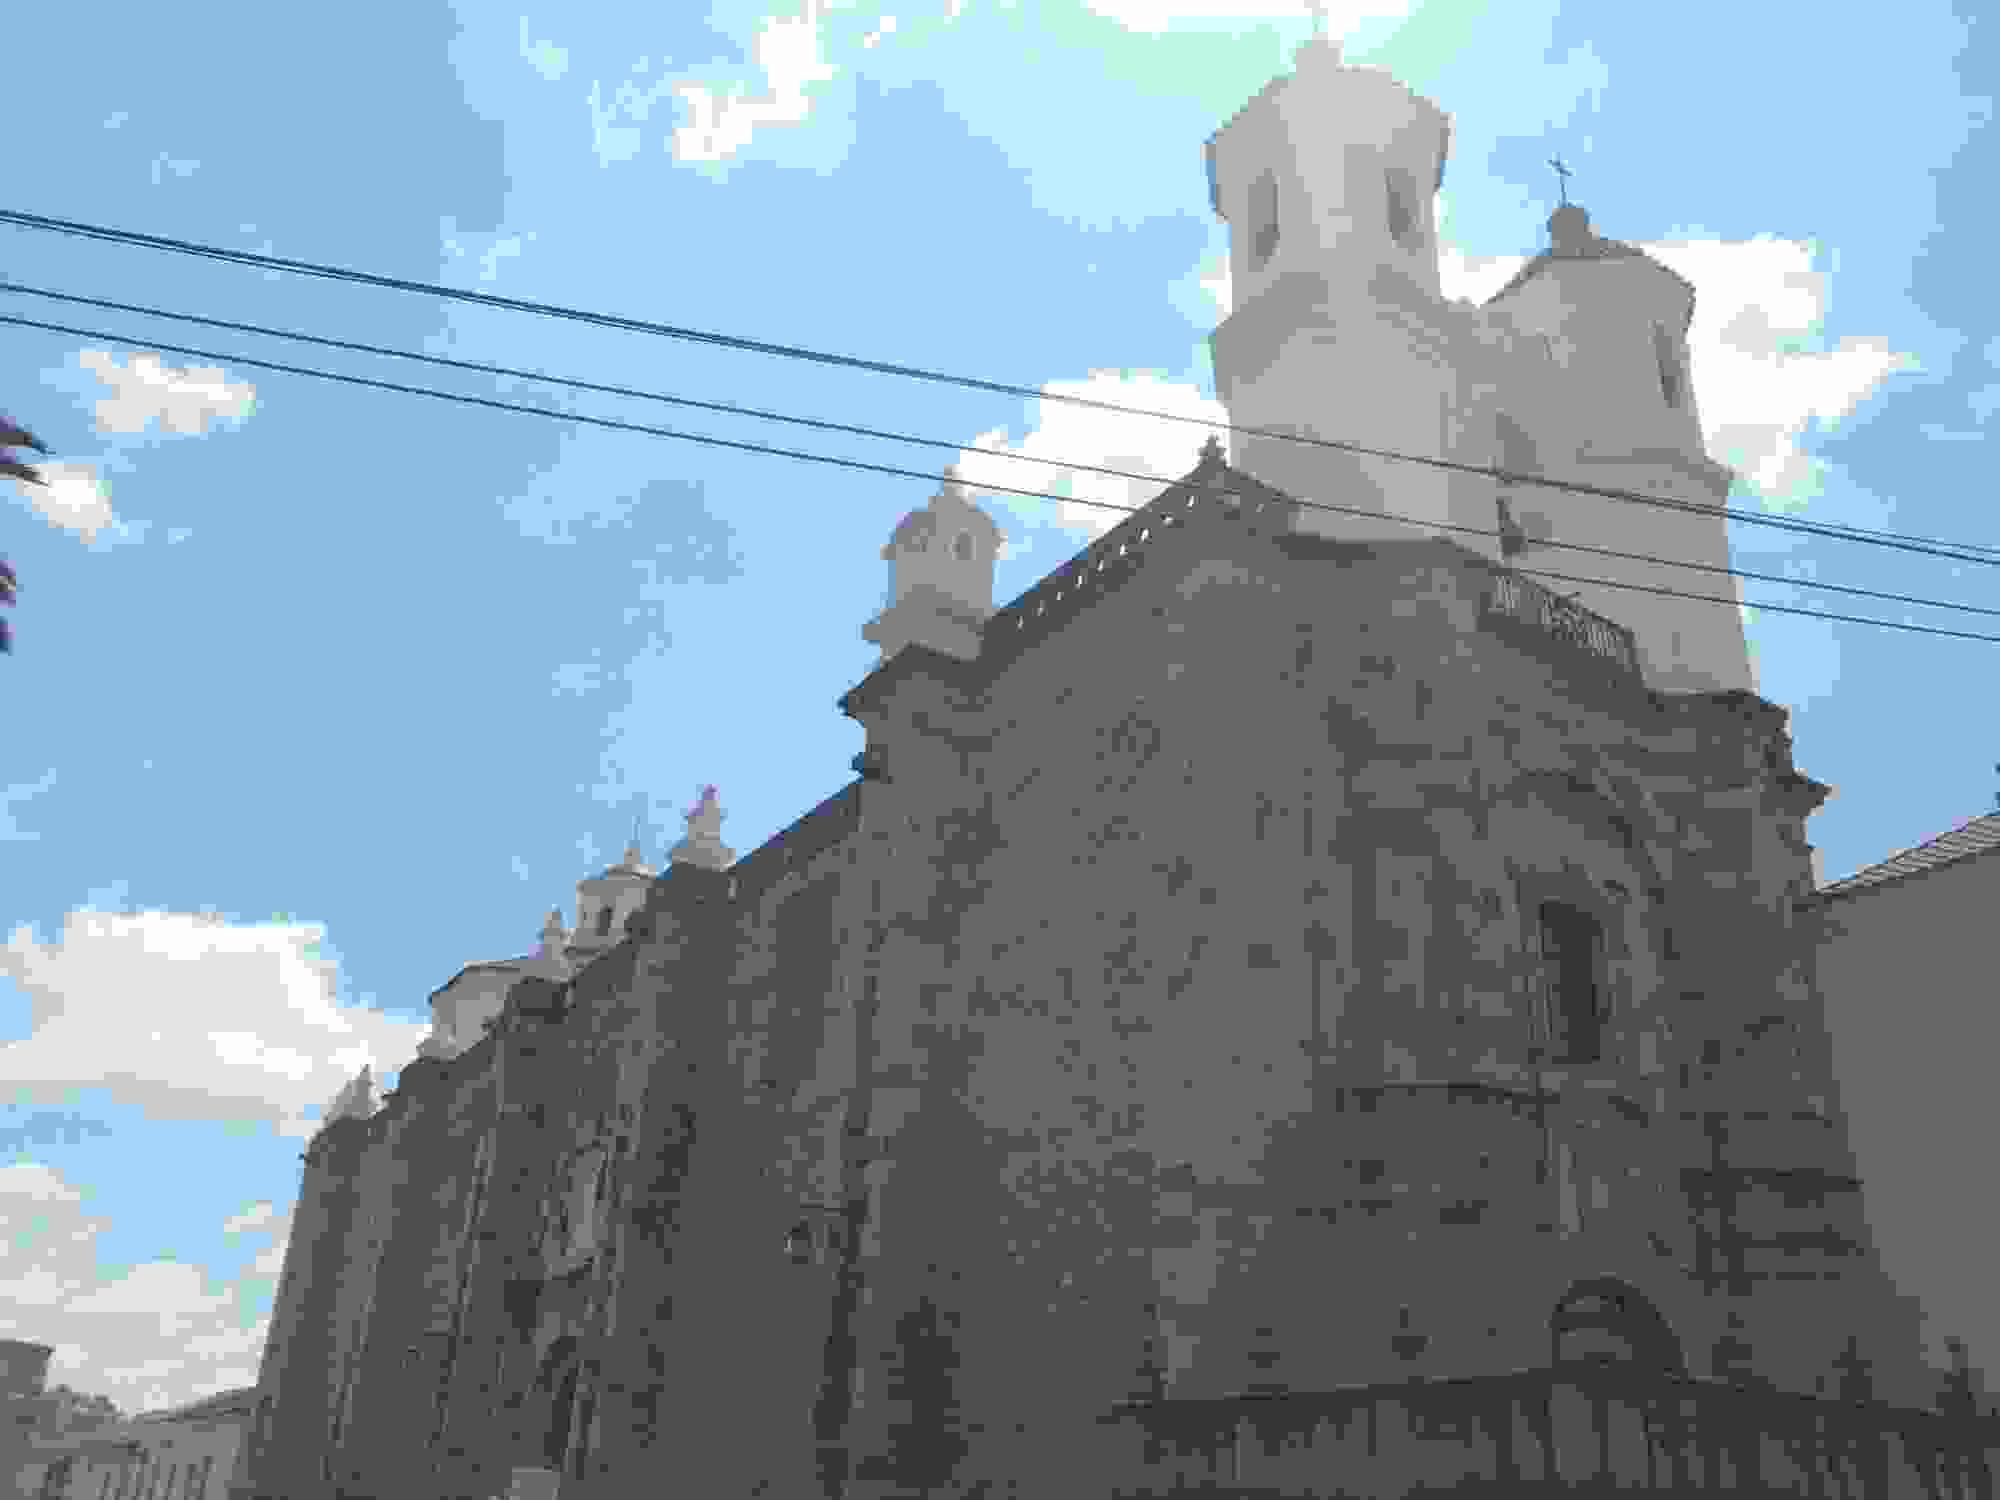
\includegraphics[width=\mywidth]{../wp-content/uploads/2015/04/wpid-wp-1429063437281.jpg} \end{center}
\begin{center} 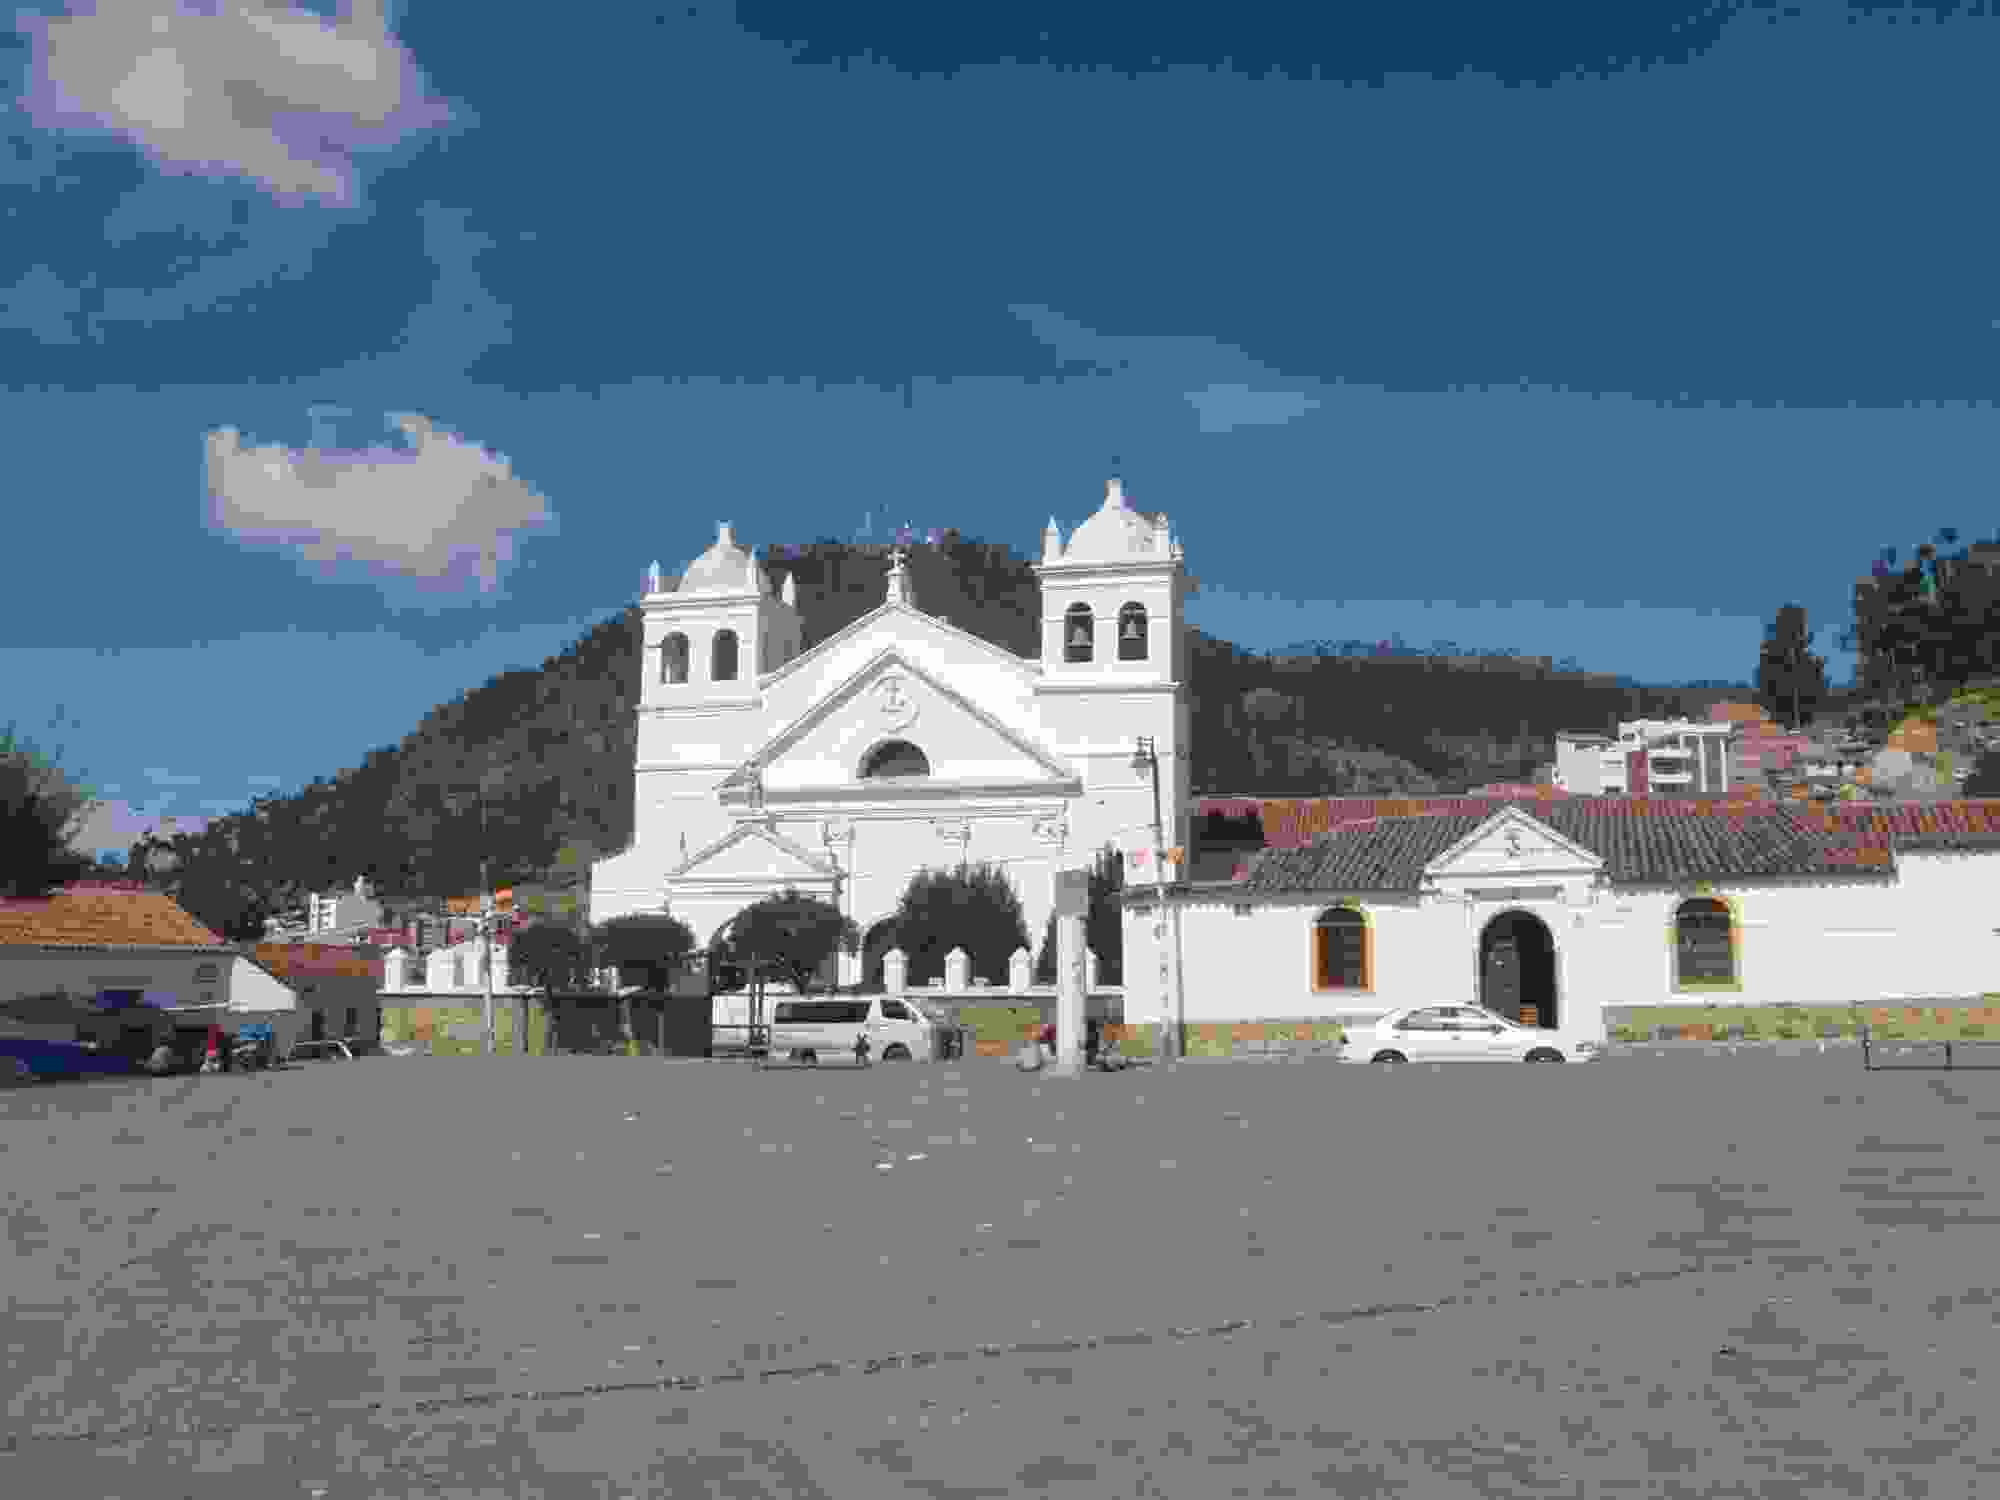
\includegraphics[width=\mywidth]{../wp-content/uploads/2015/04/wpid-wp-1429063894588.jpg} \end{center}

 Le marché central de Sucre, une merveille on trouve de tout. 
\begin{center} 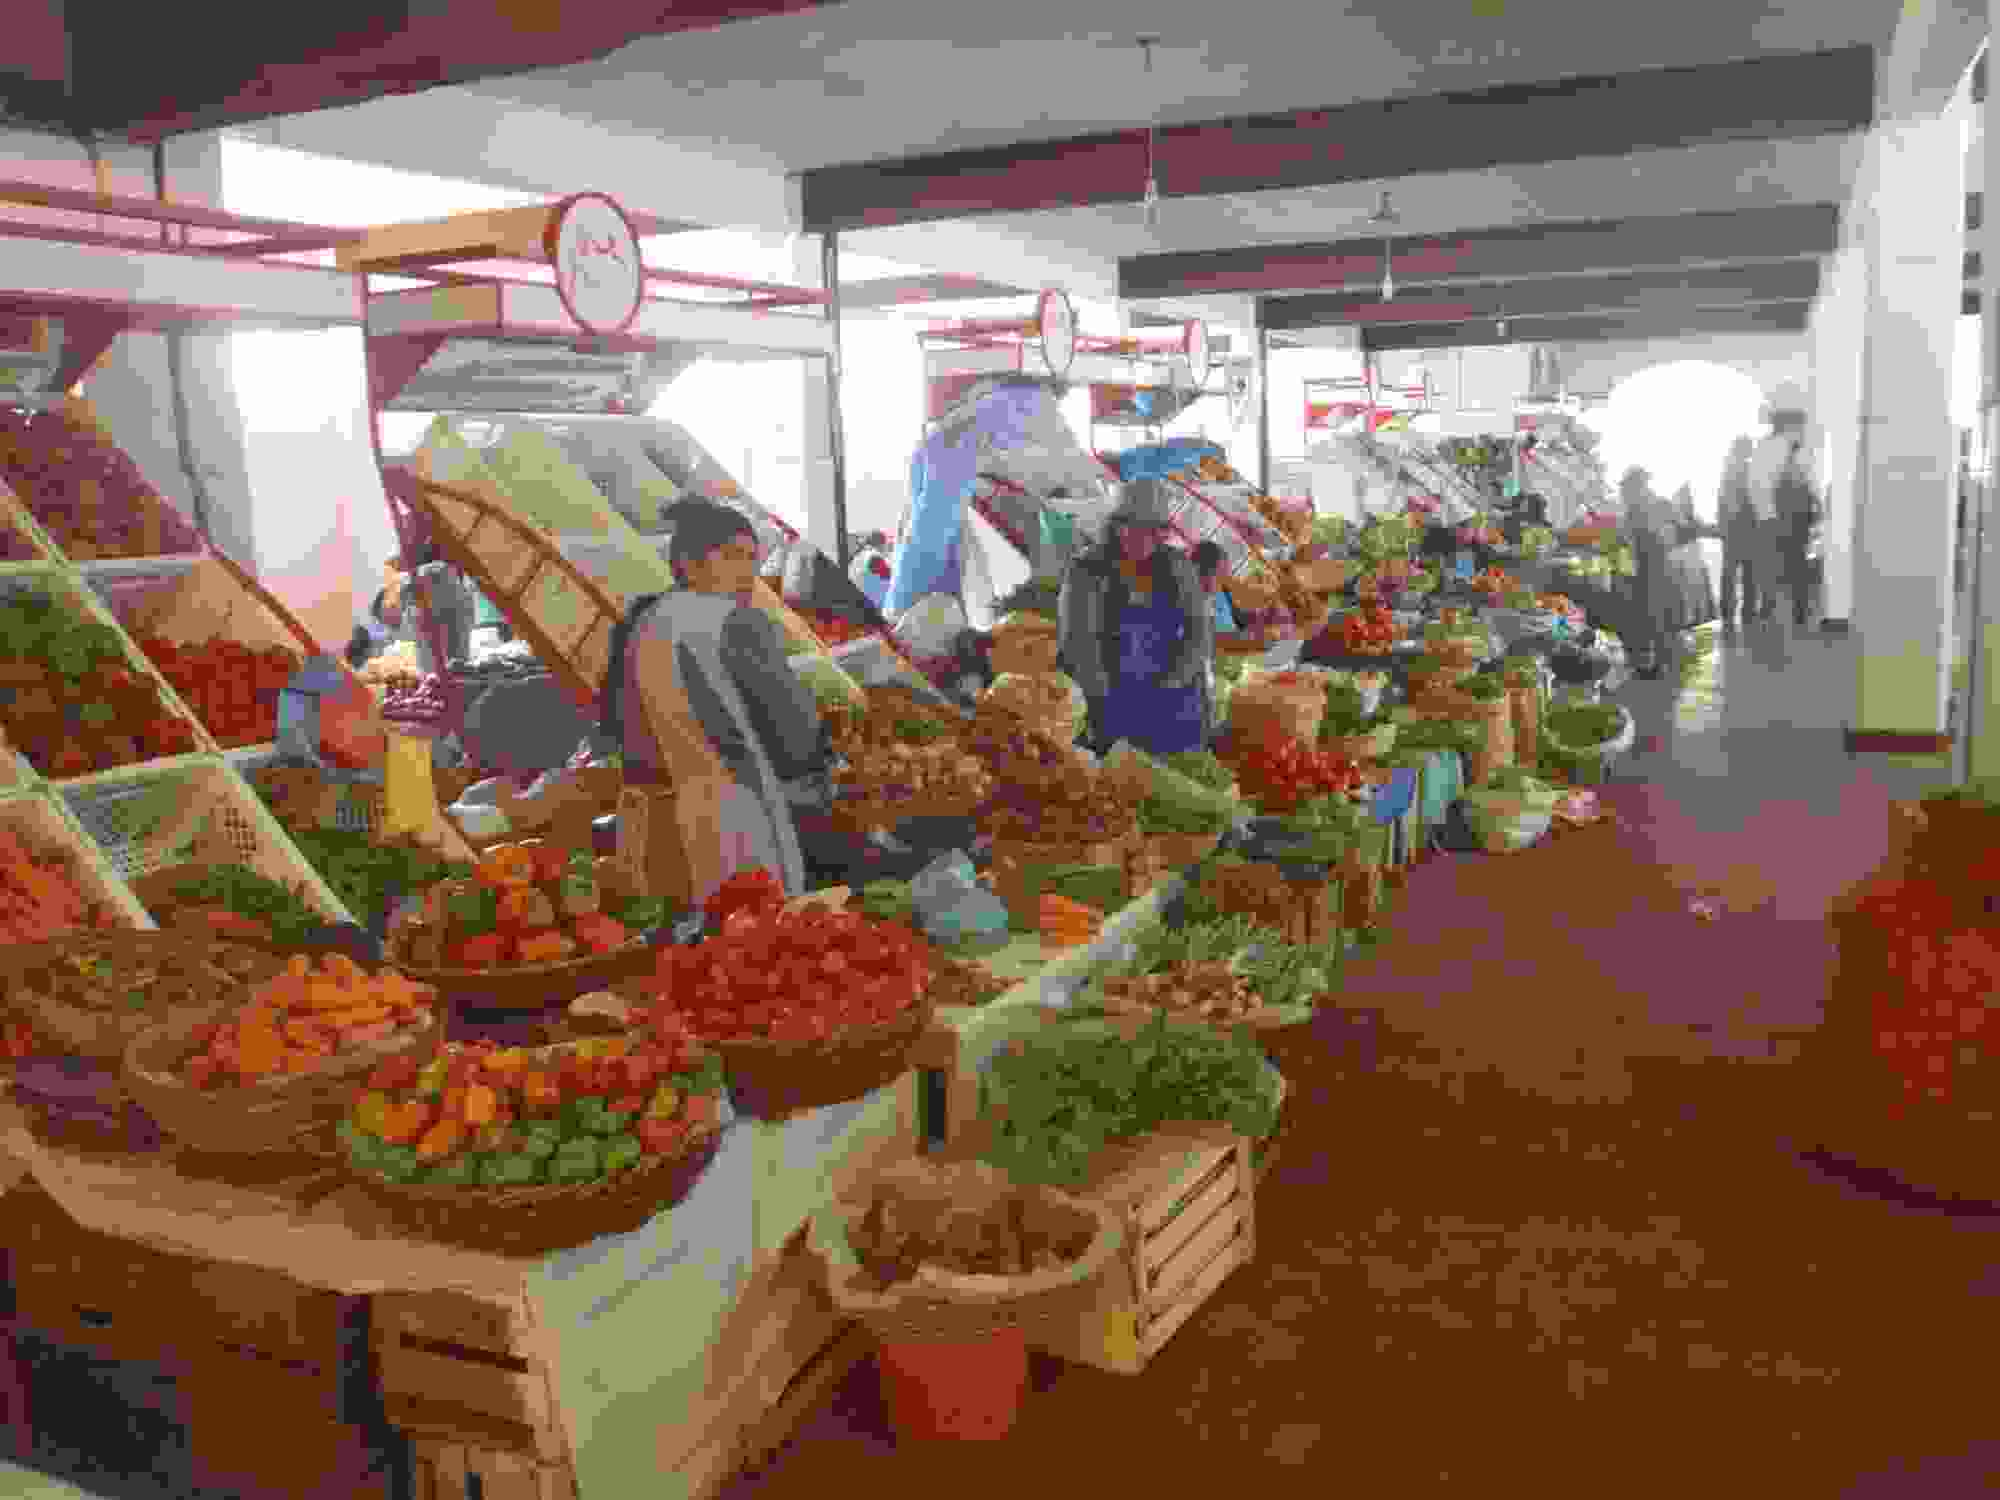
\includegraphics[width=\mywidth]{../wp-content/uploads/2015/04/wpid-wp-1429062883937.jpg} \end{center}
\begin{center} 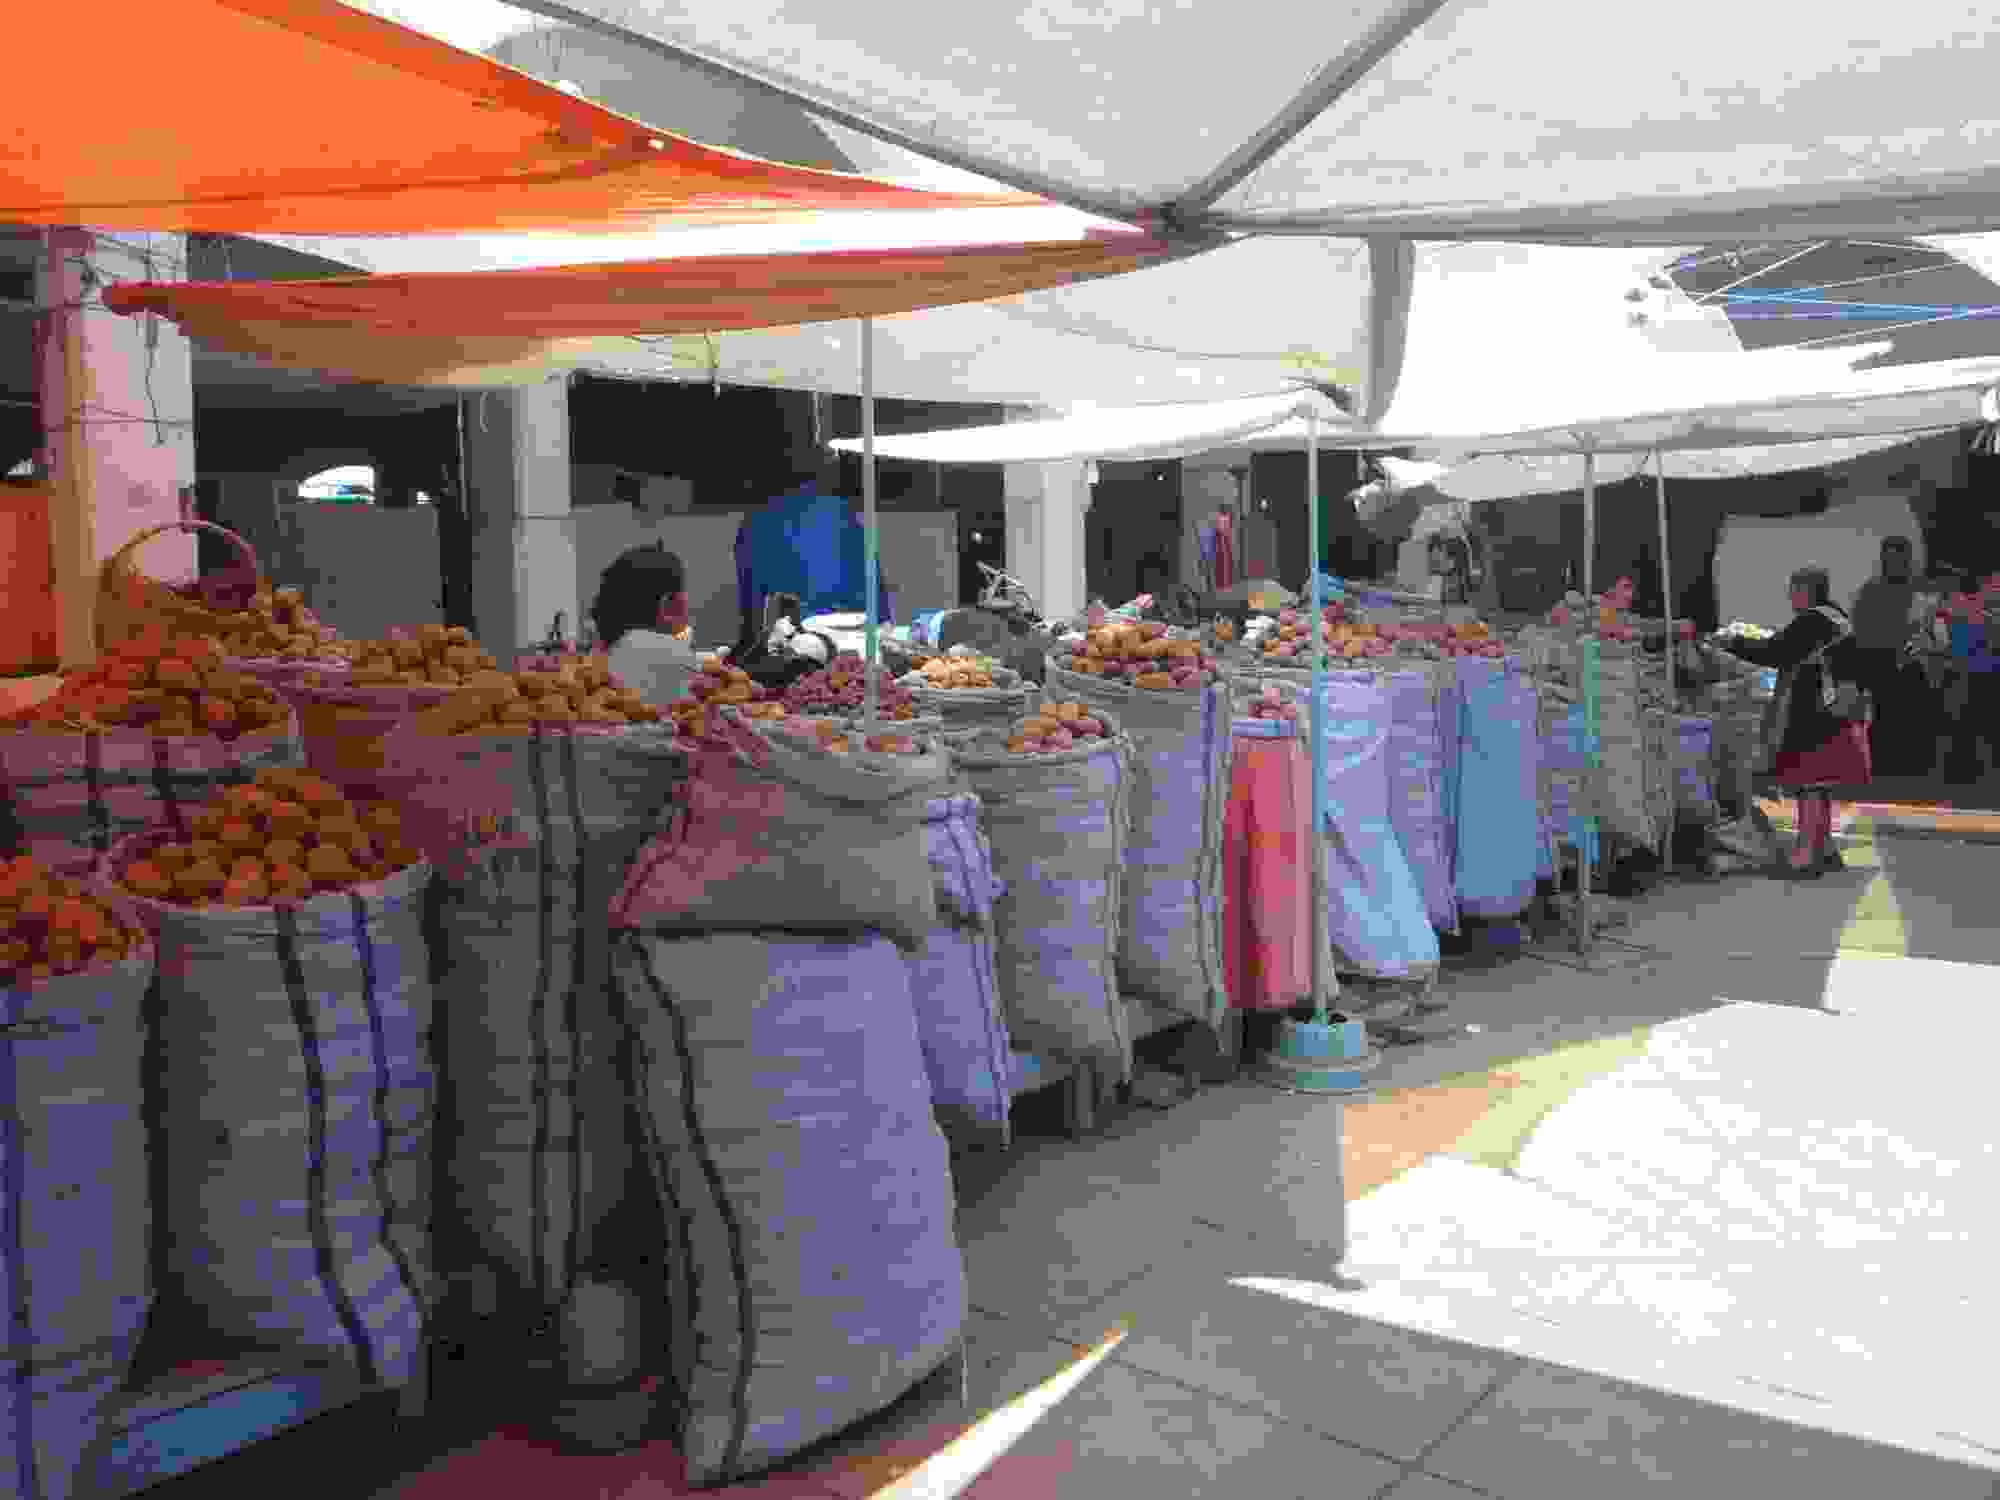
\includegraphics[width=\mywidth]{../wp-content/uploads/2015/04/wpid-wp-1429062898209.jpg} \end{center}
\begin{center} 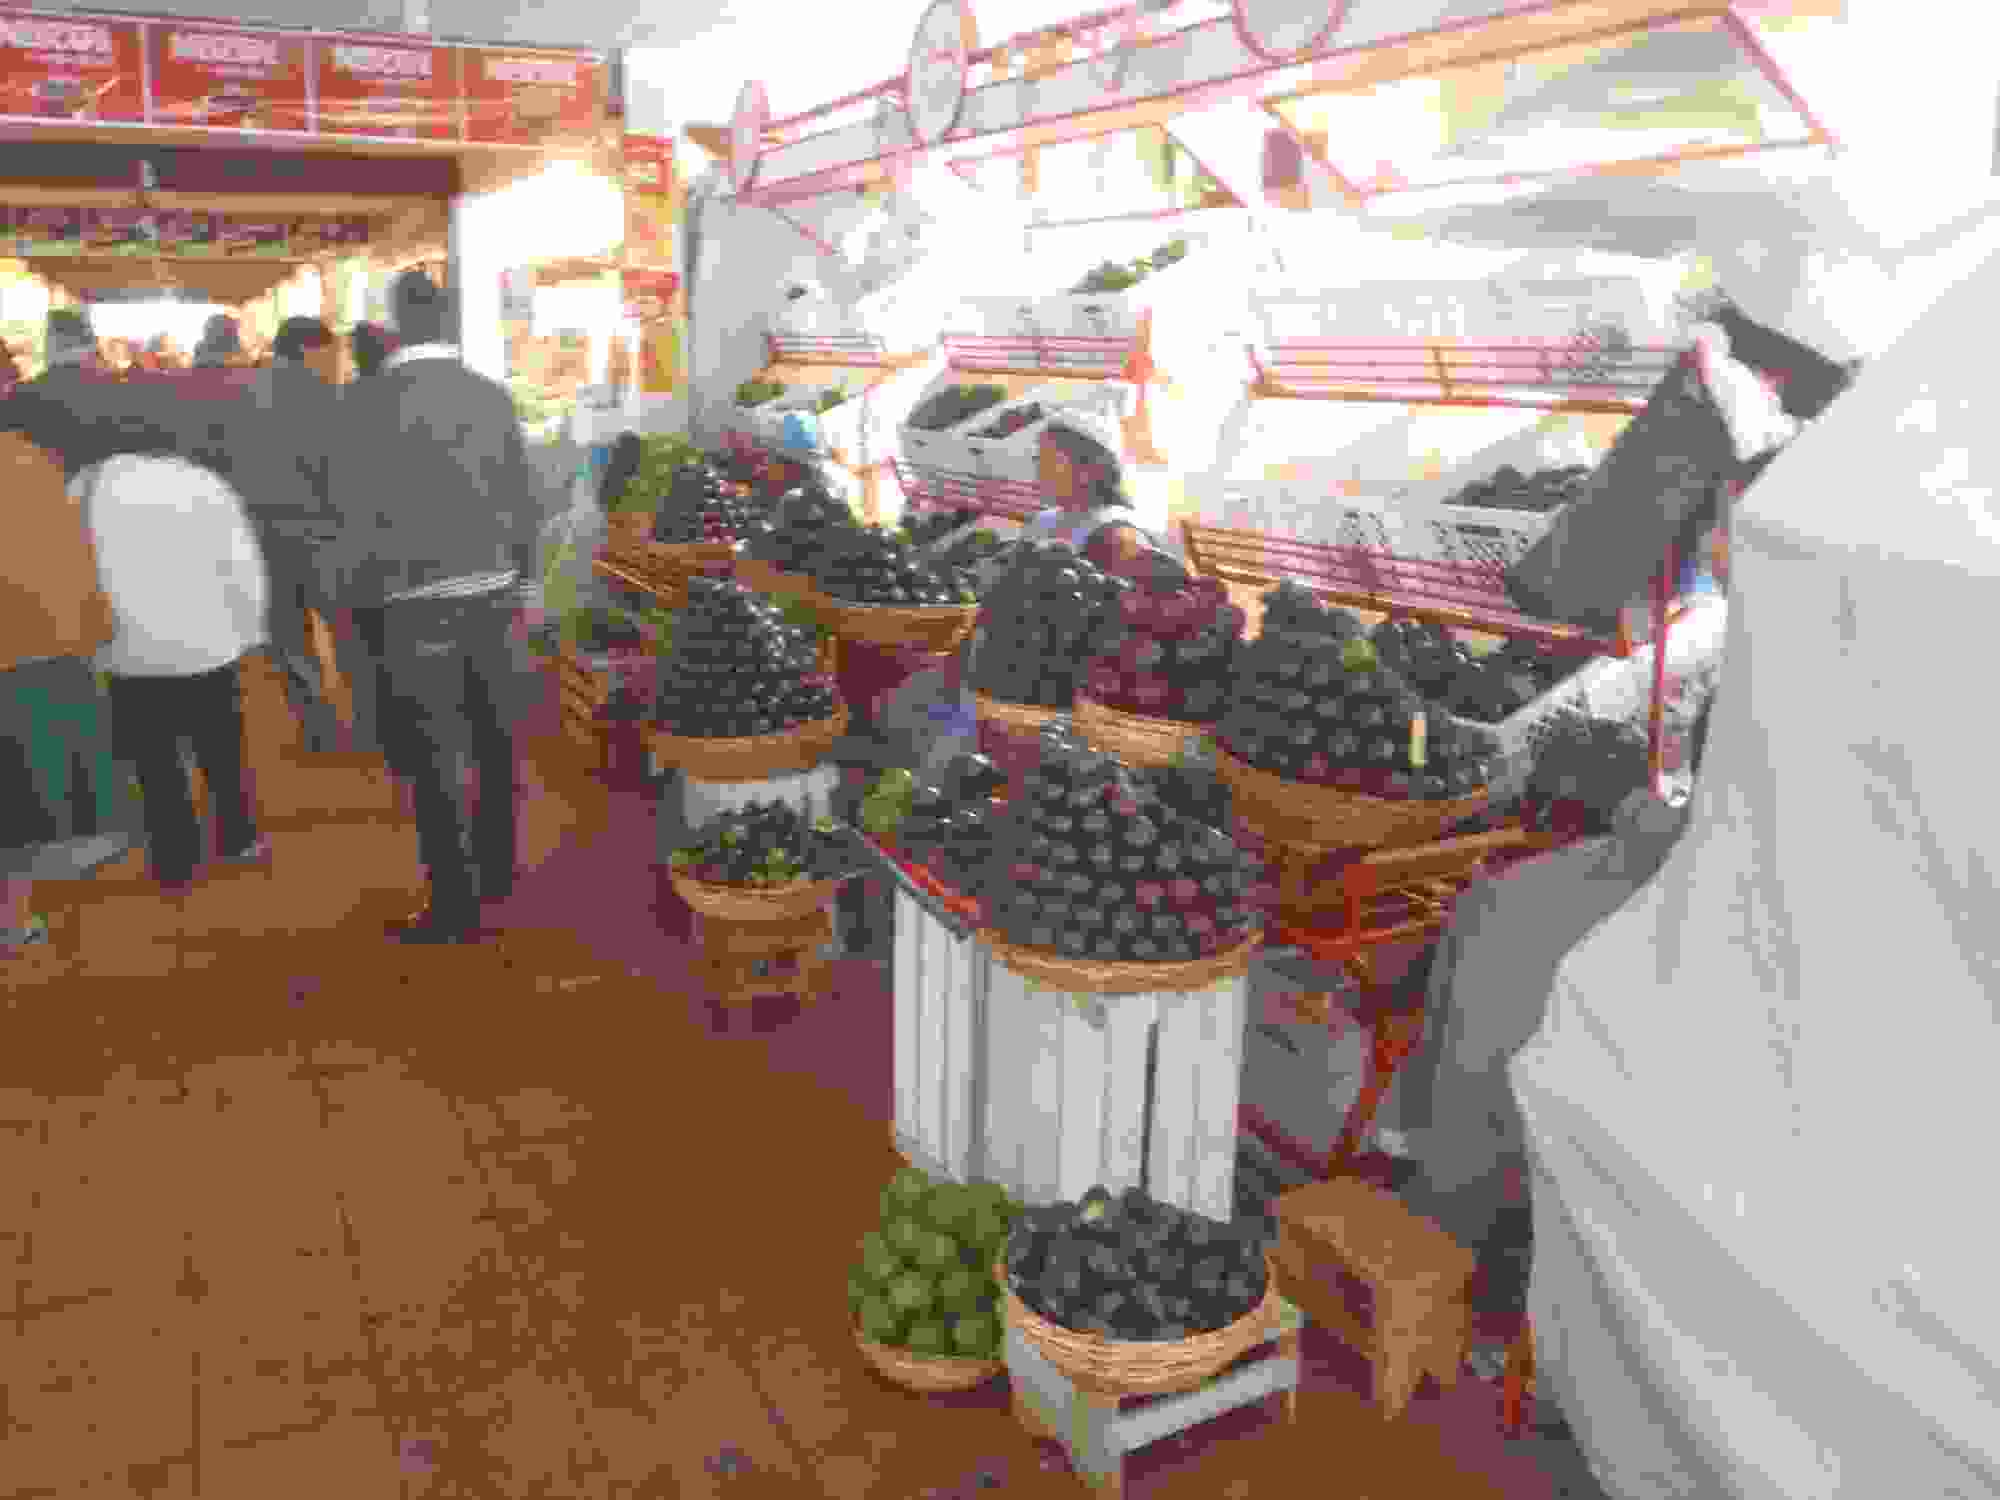
\includegraphics[width=\mywidth]{../wp-content/uploads/2015/04/wpid-wp-1429062910596.jpg} \end{center}
\begin{center} 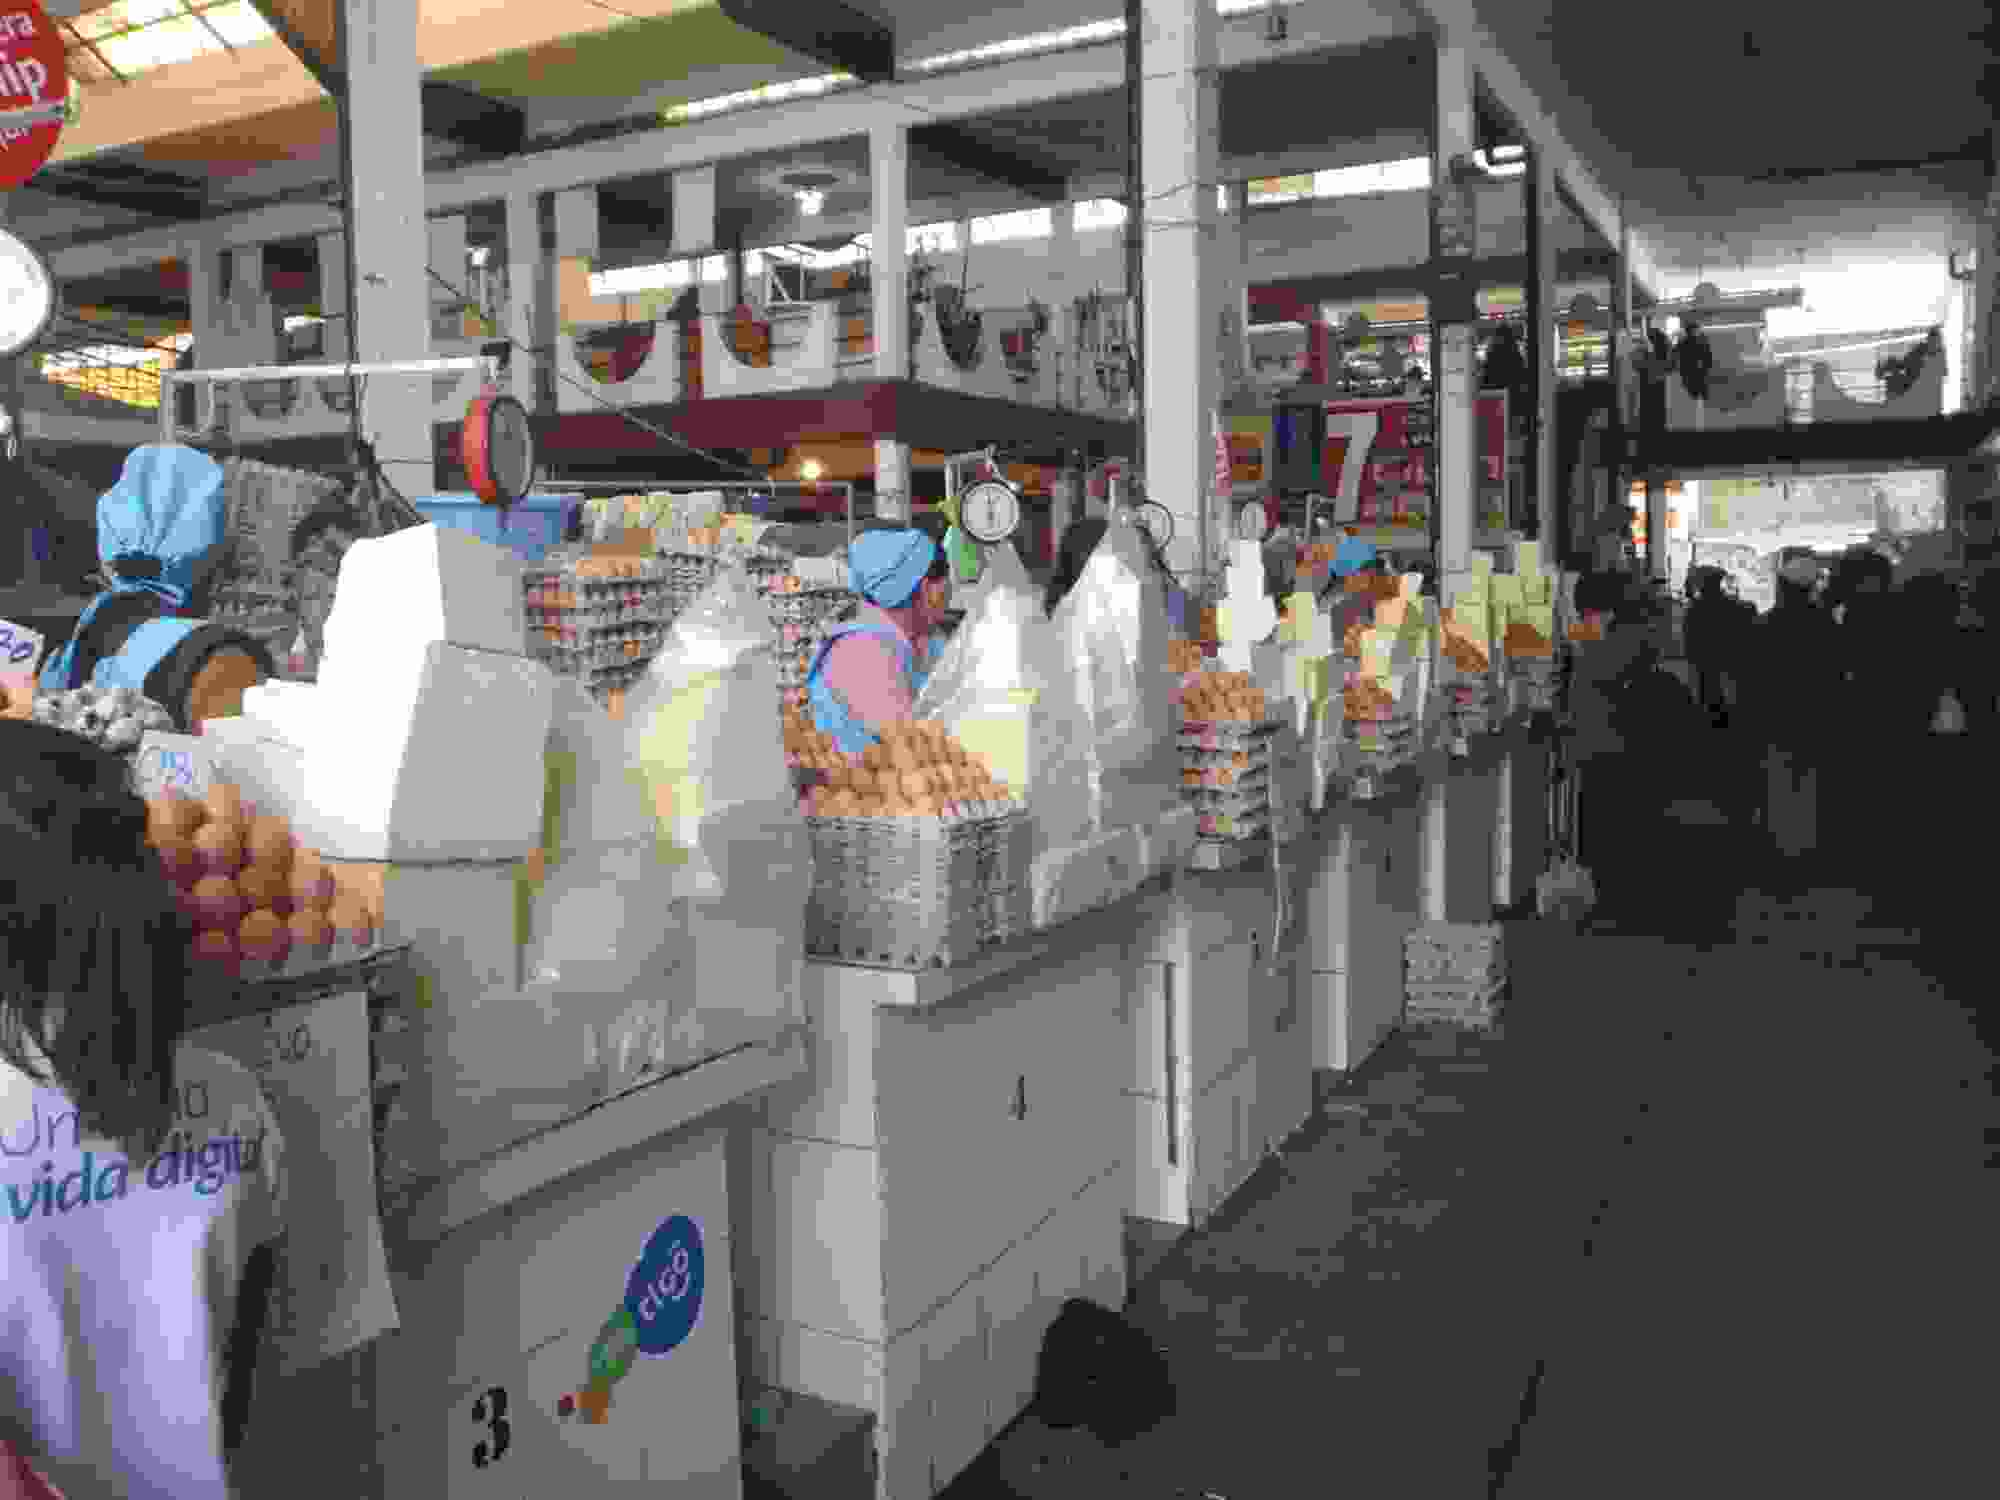
\includegraphics[width=\mywidth]{../wp-content/uploads/2015/04/wpid-wp-1429062969618.jpg} \end{center}
\begin{center} 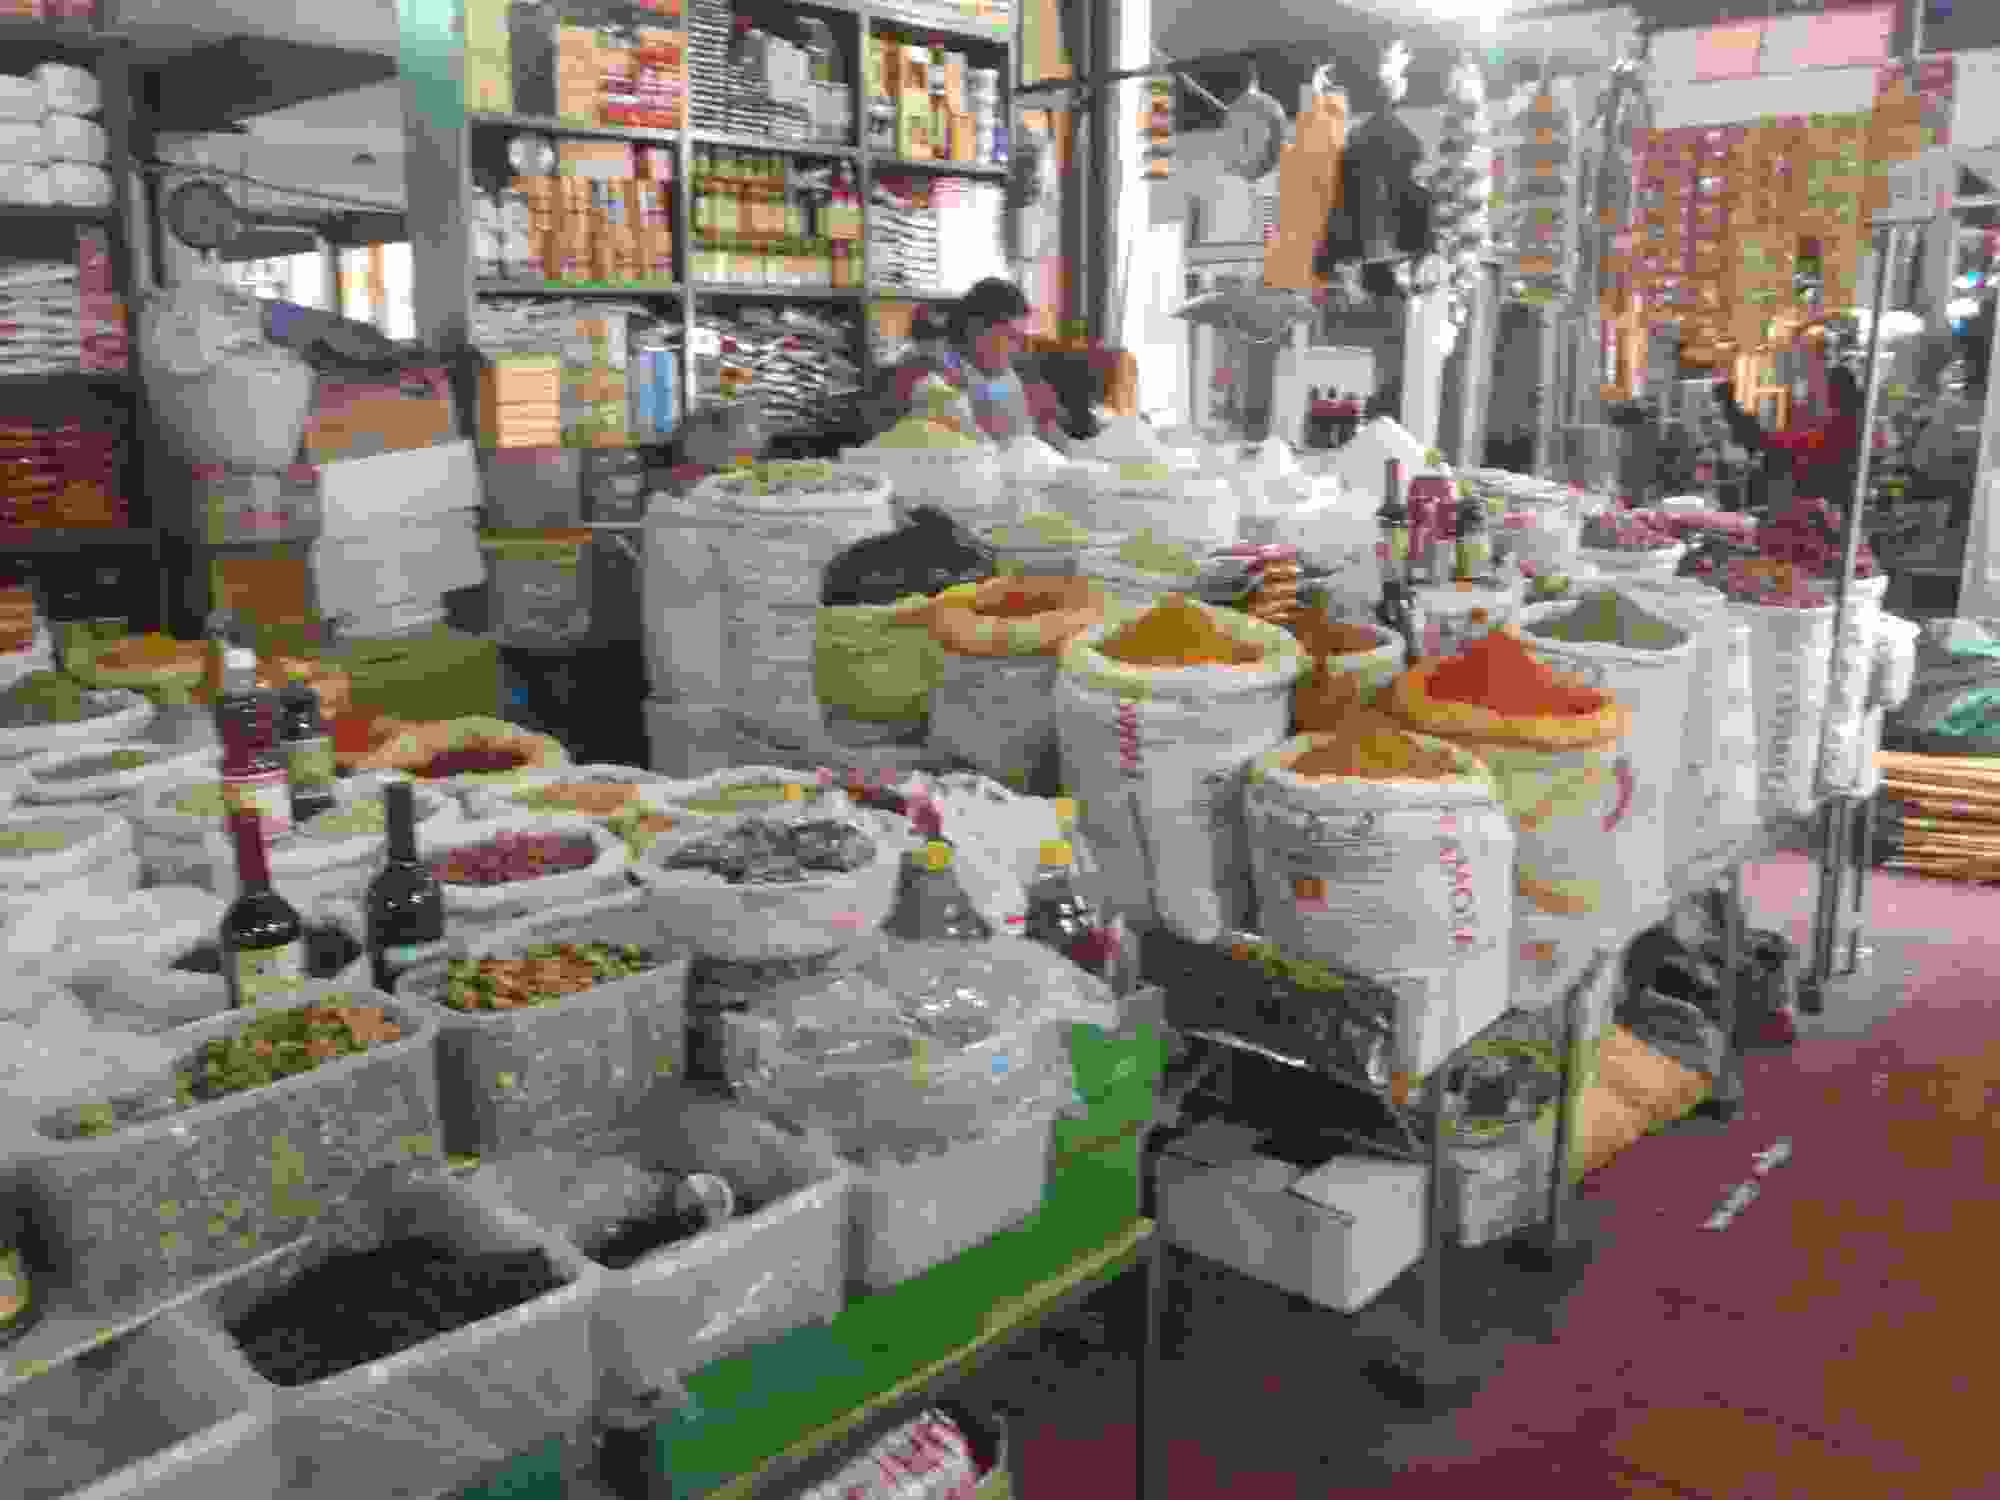
\includegraphics[width=\mywidth]{../wp-content/uploads/2015/04/wpid-wp-1429062996837.jpg} \end{center}
\begin{center} 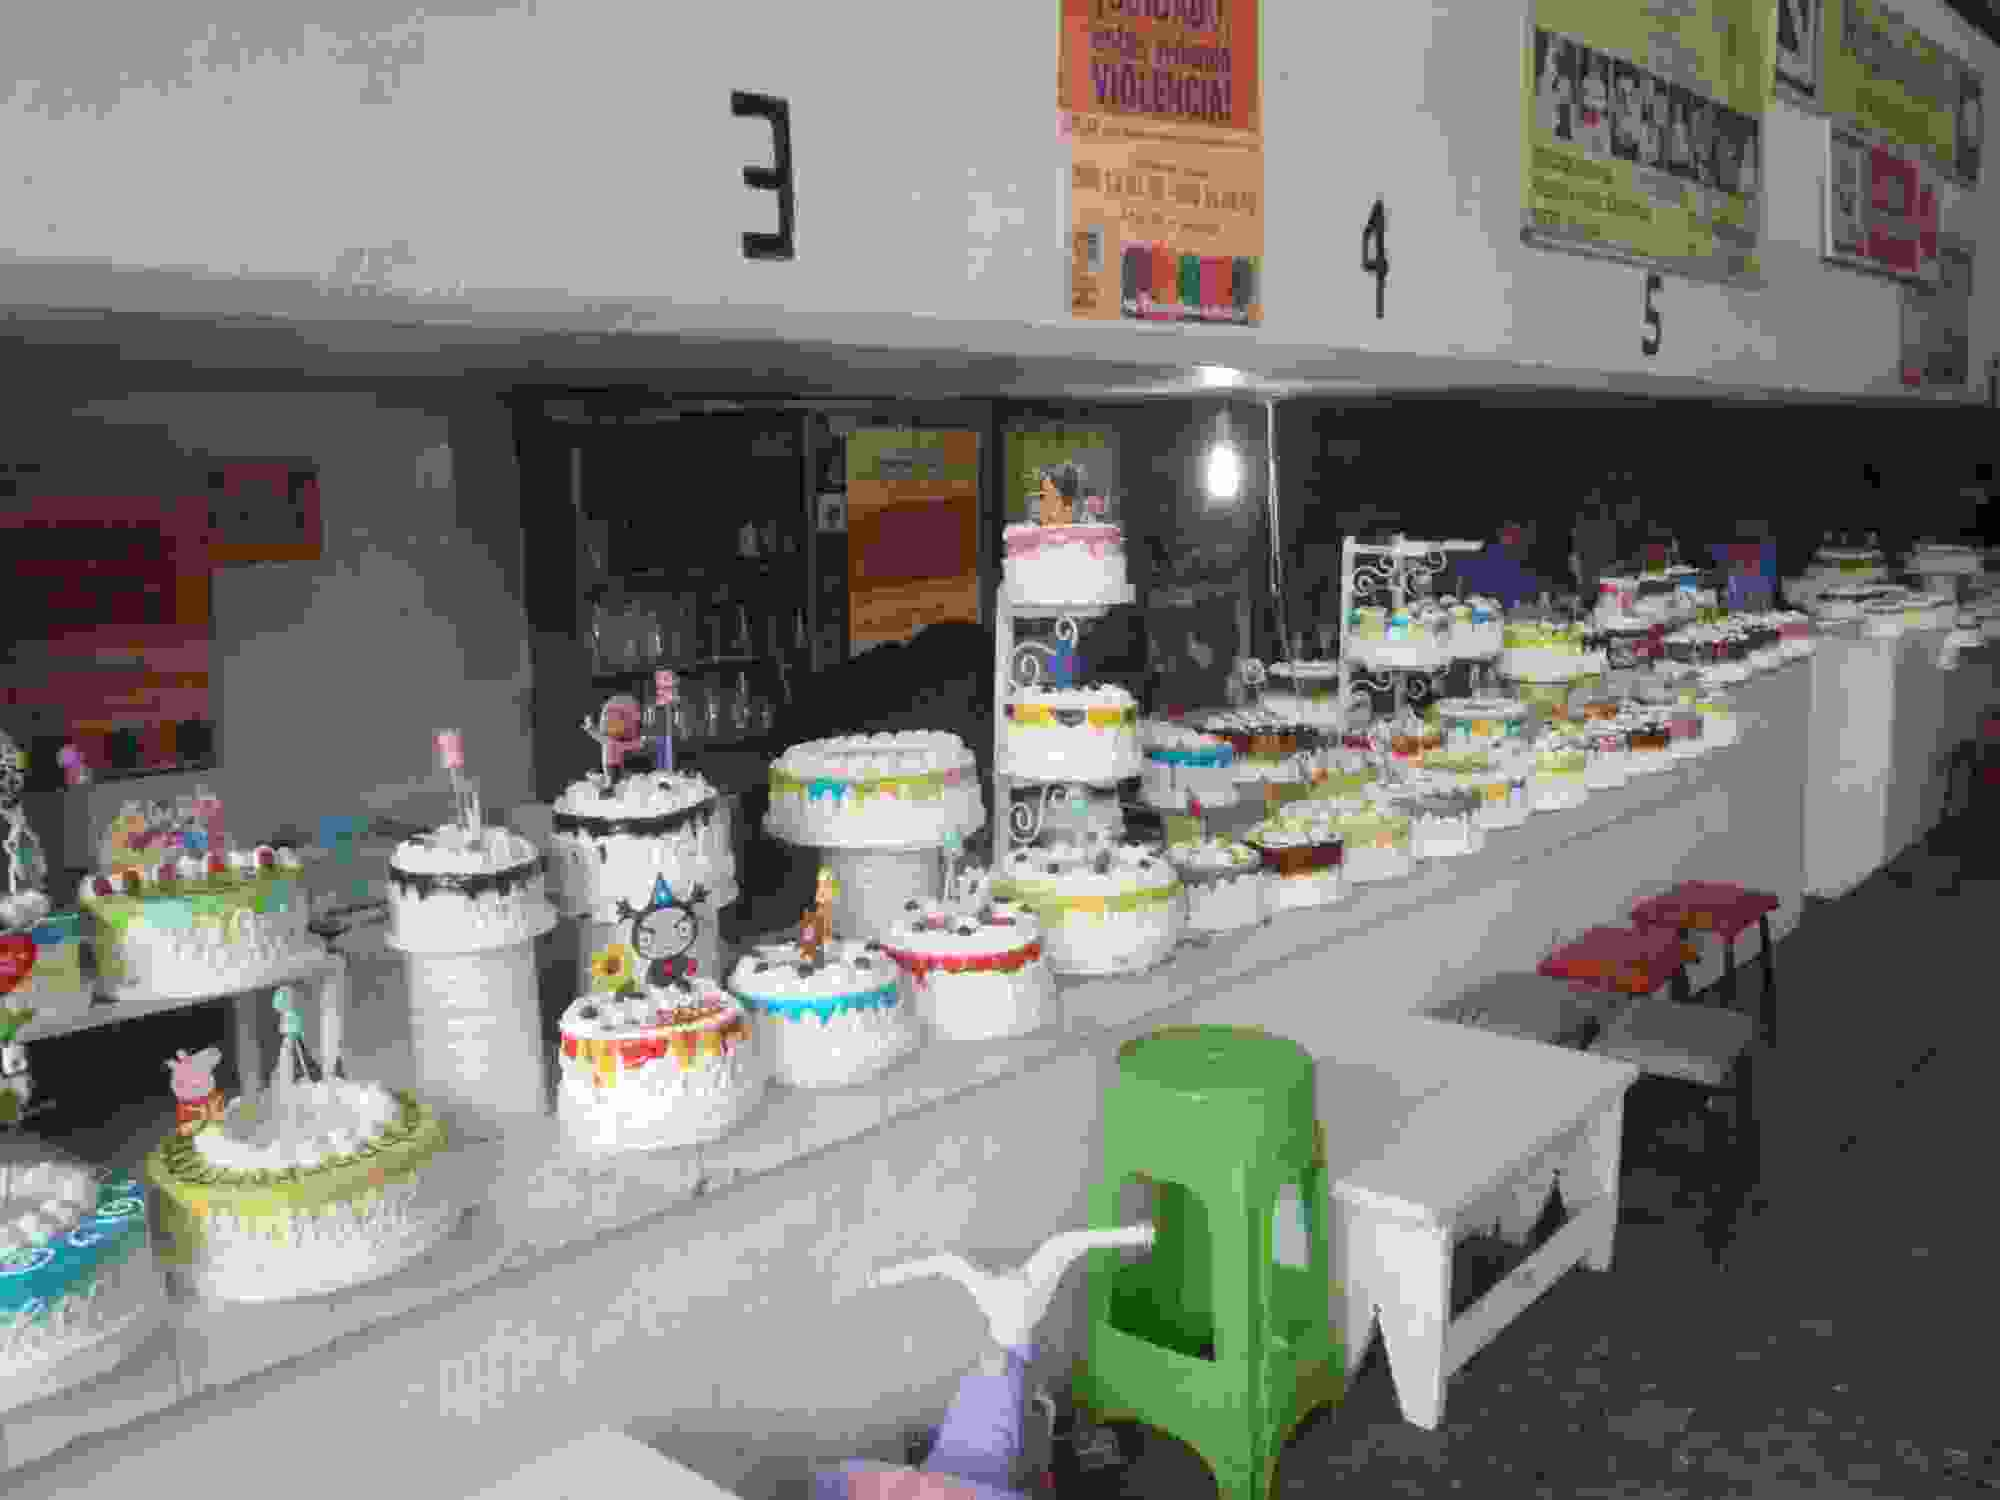
\includegraphics[width=\mywidth]{../wp-content/uploads/2015/04/wpid-wp-1429063009158.jpg} \end{center}

  Les stands qui servent des jus et des salades de fruits : un régal et pas cher. 
\begin{center} 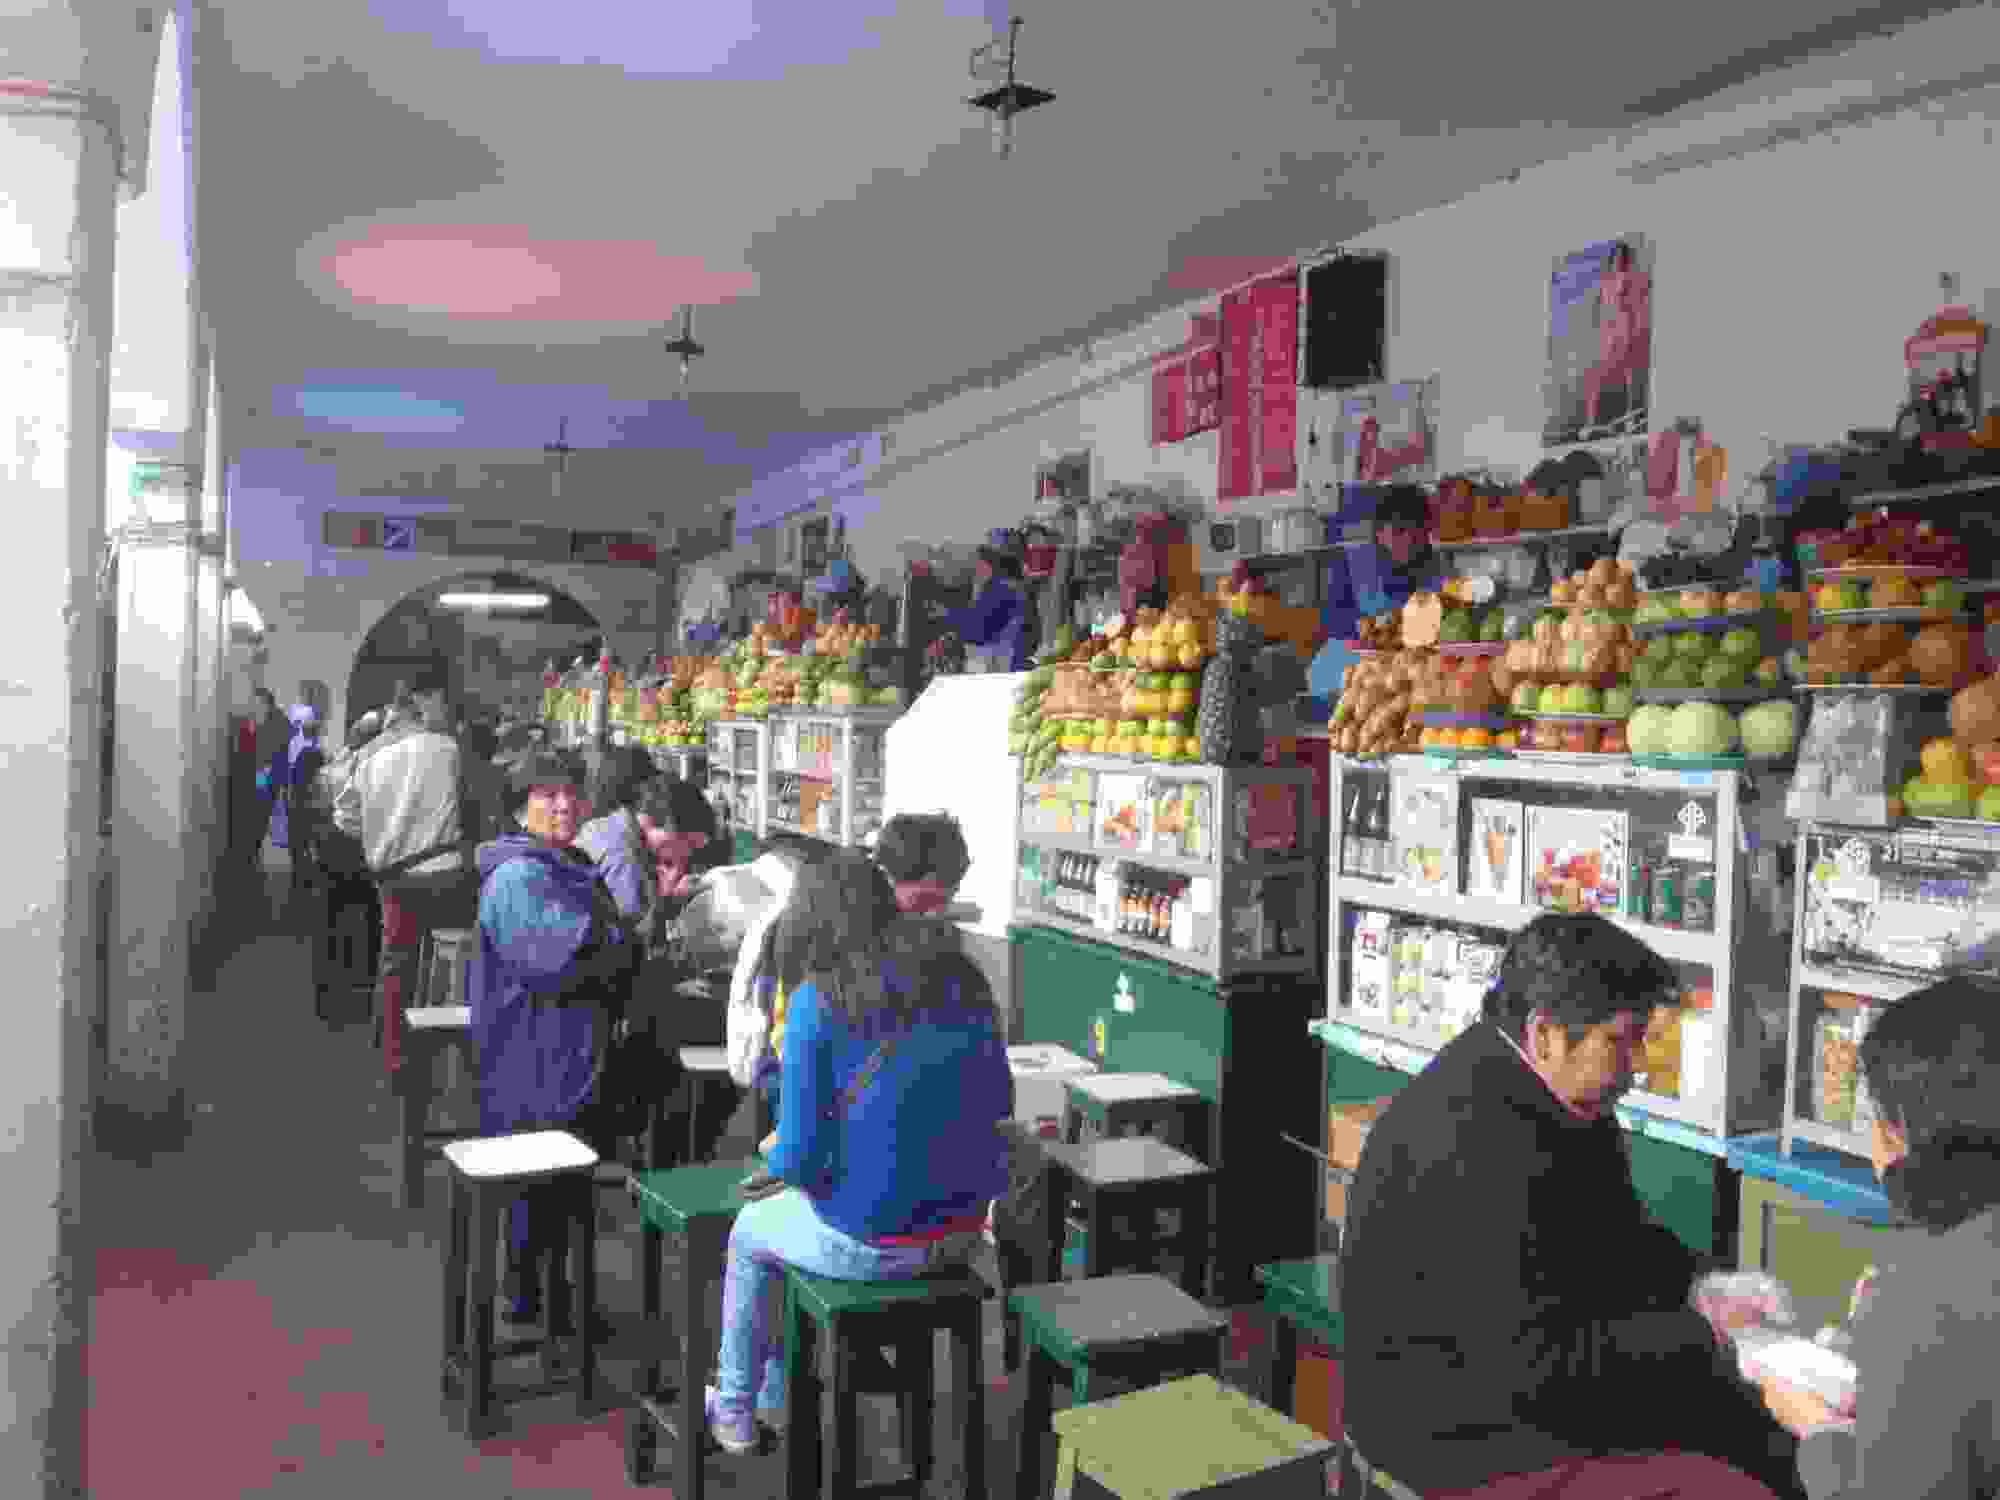
\includegraphics[width=\mywidth]{../wp-content/uploads/2015/04/wpid-wp-1429063121415.jpg} \end{center}
\vspace{-\topsep}

\pagebreak
~
\begin{center} 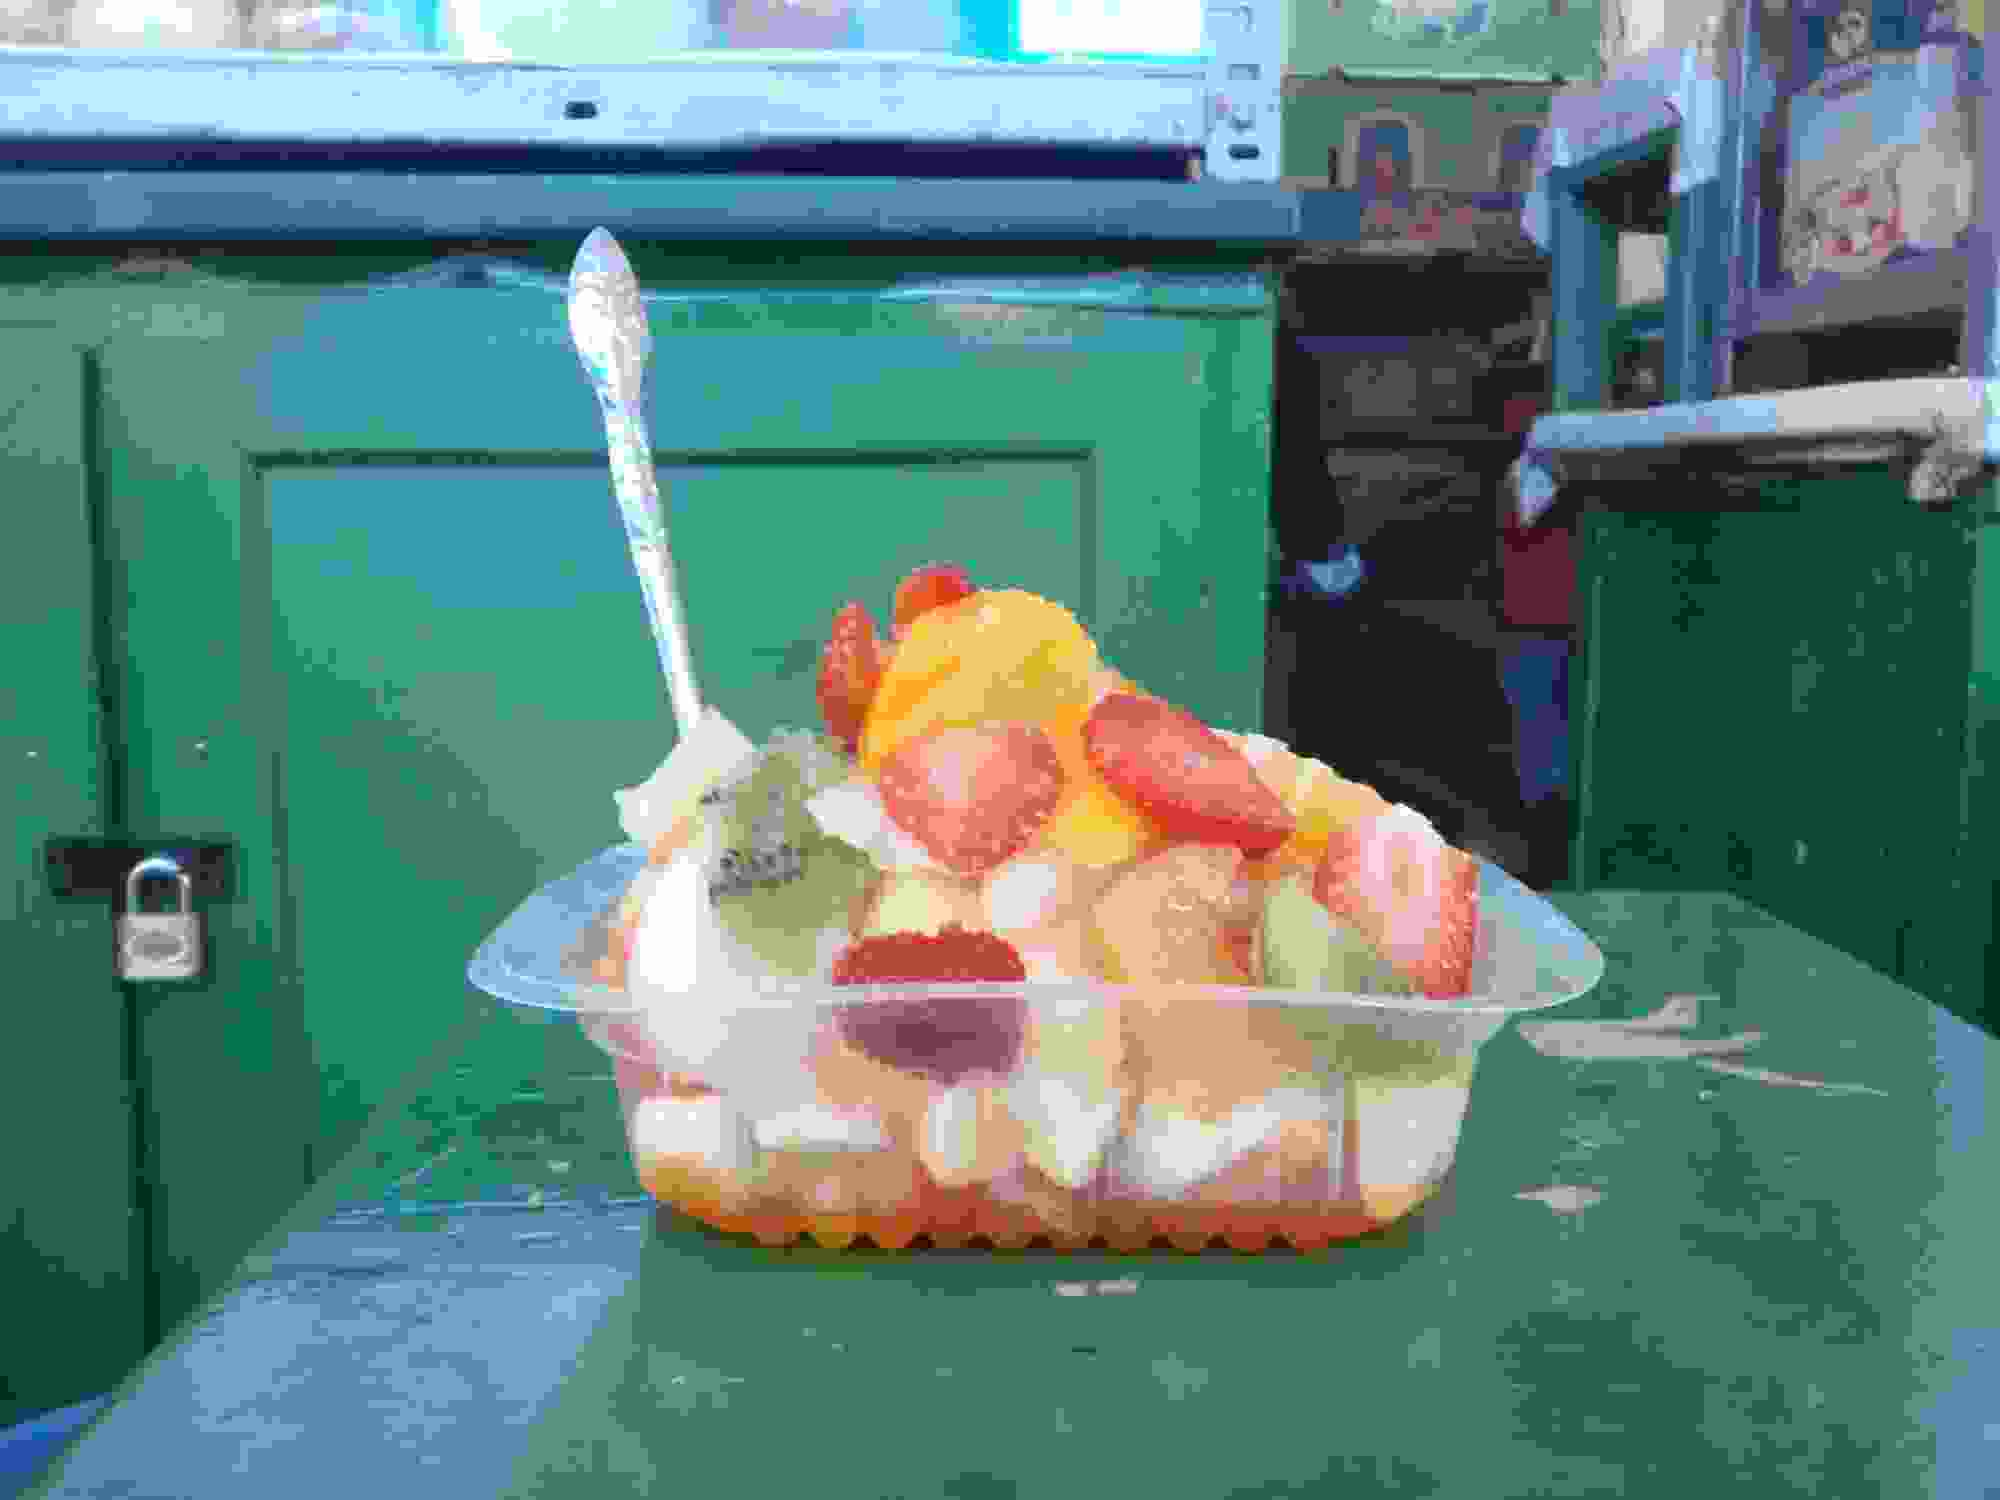
\includegraphics[width=\mywidth]{../wp-content/uploads/2015/04/wpid-wp-1429063146866.jpg} \end{center}

 La Recoleta, un beau point de vue sur la ville :
\begin{center} 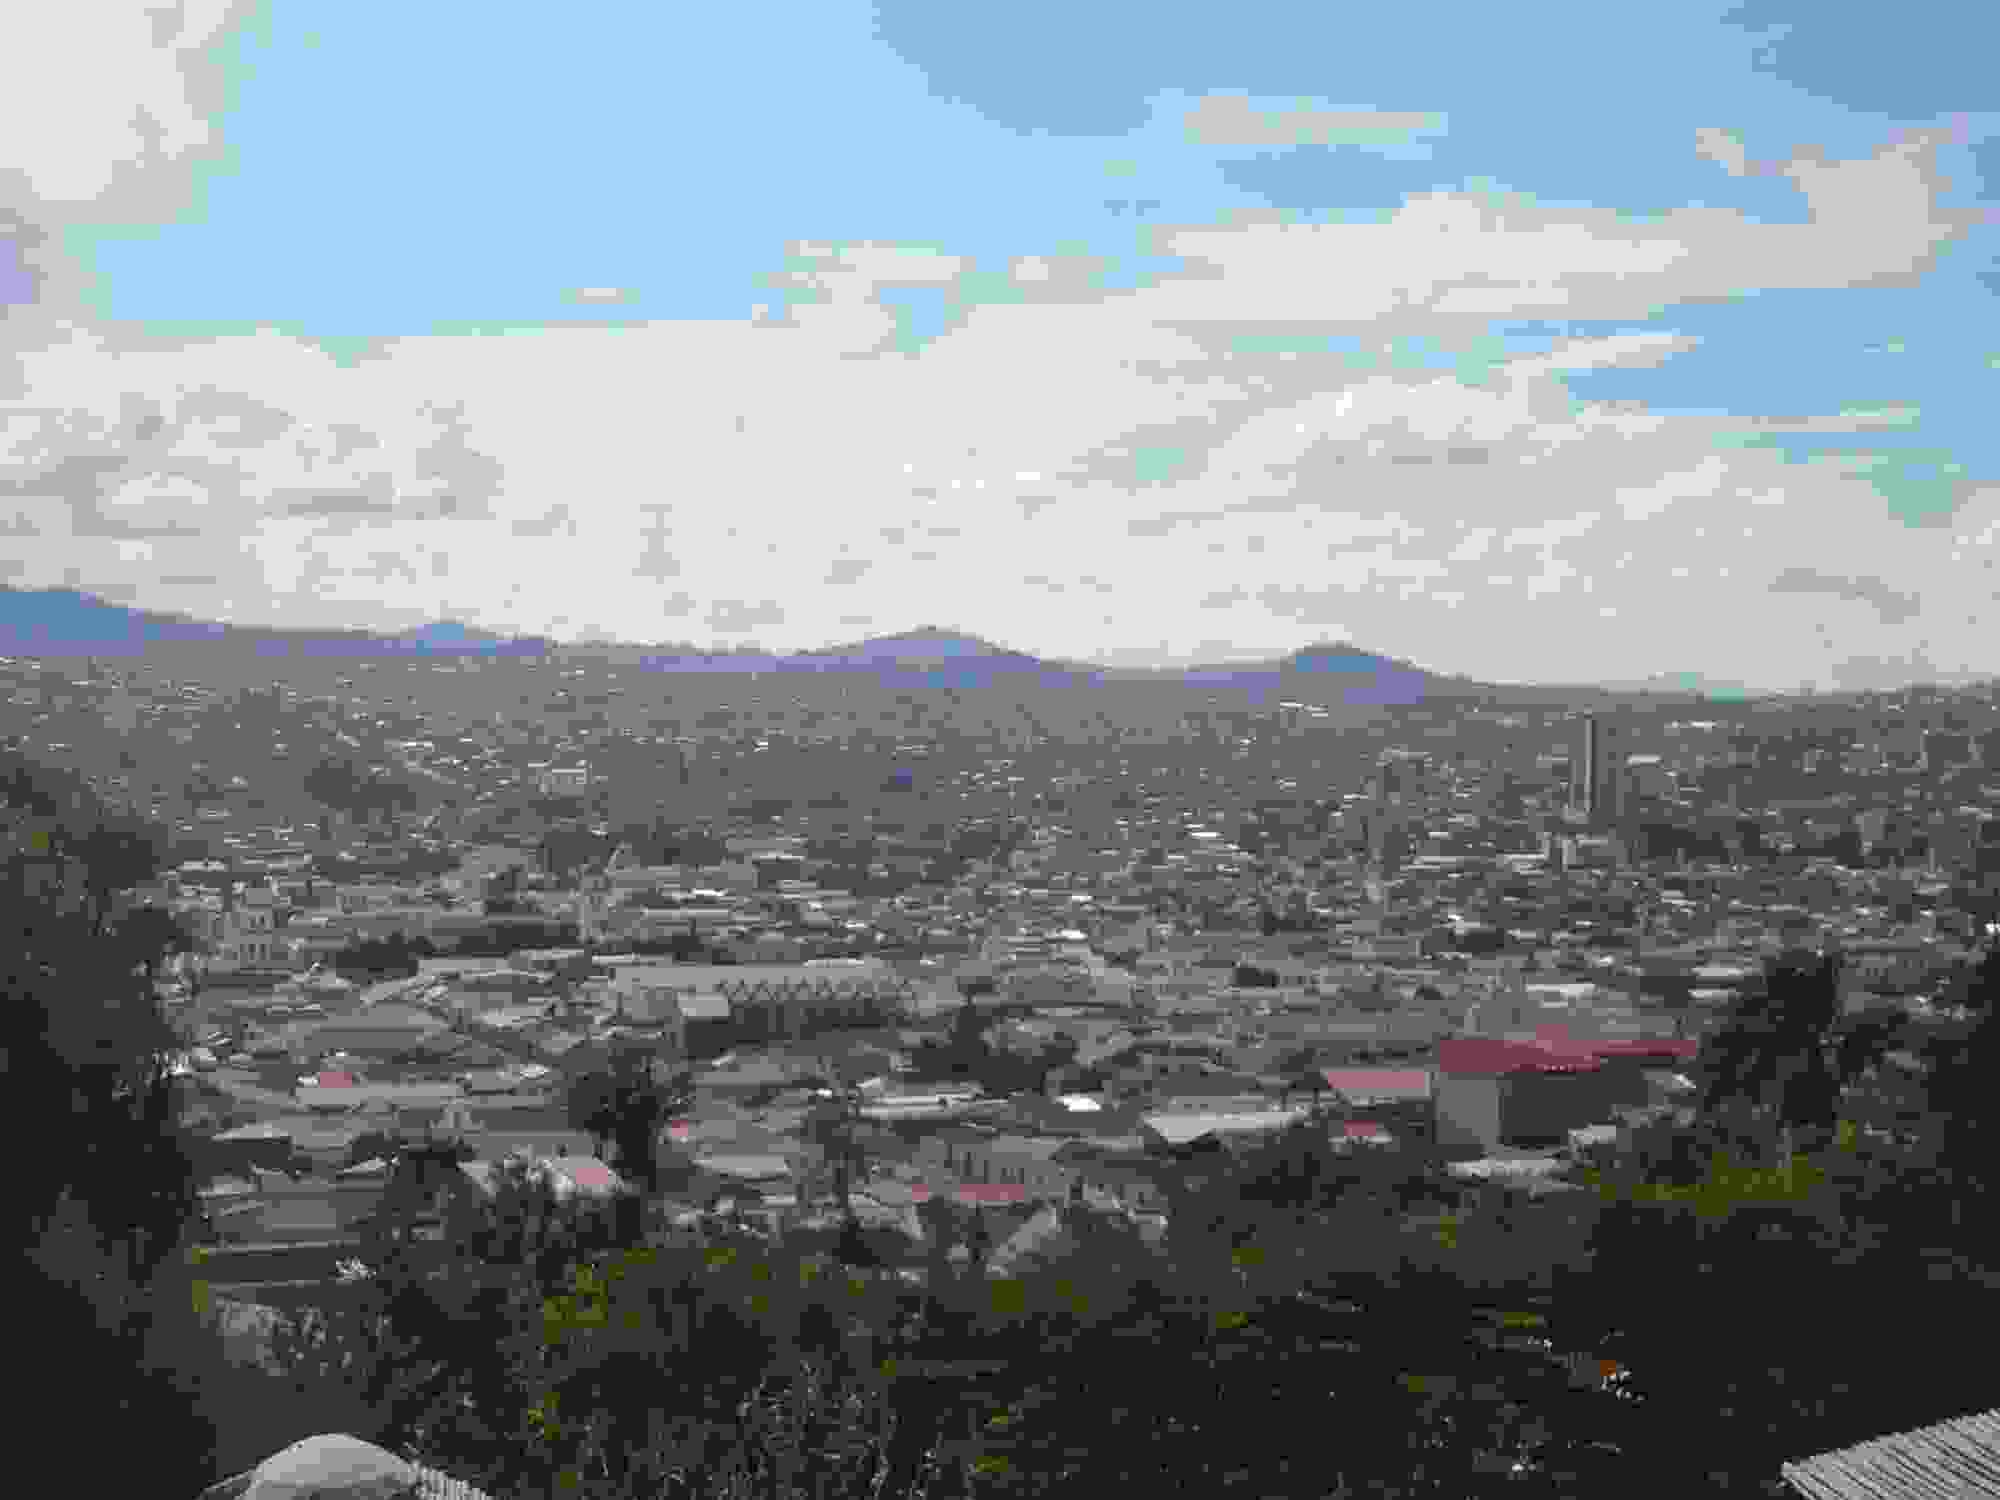
\includegraphics[width=\mywidth]{../wp-content/uploads/2015/04/wpid-wp-1429063611807.jpg} \end{center}
\vspace{-\topsep}

\pagebreak
 Le parc Bolivar et sa mini tour Eiffel :
\begin{center} 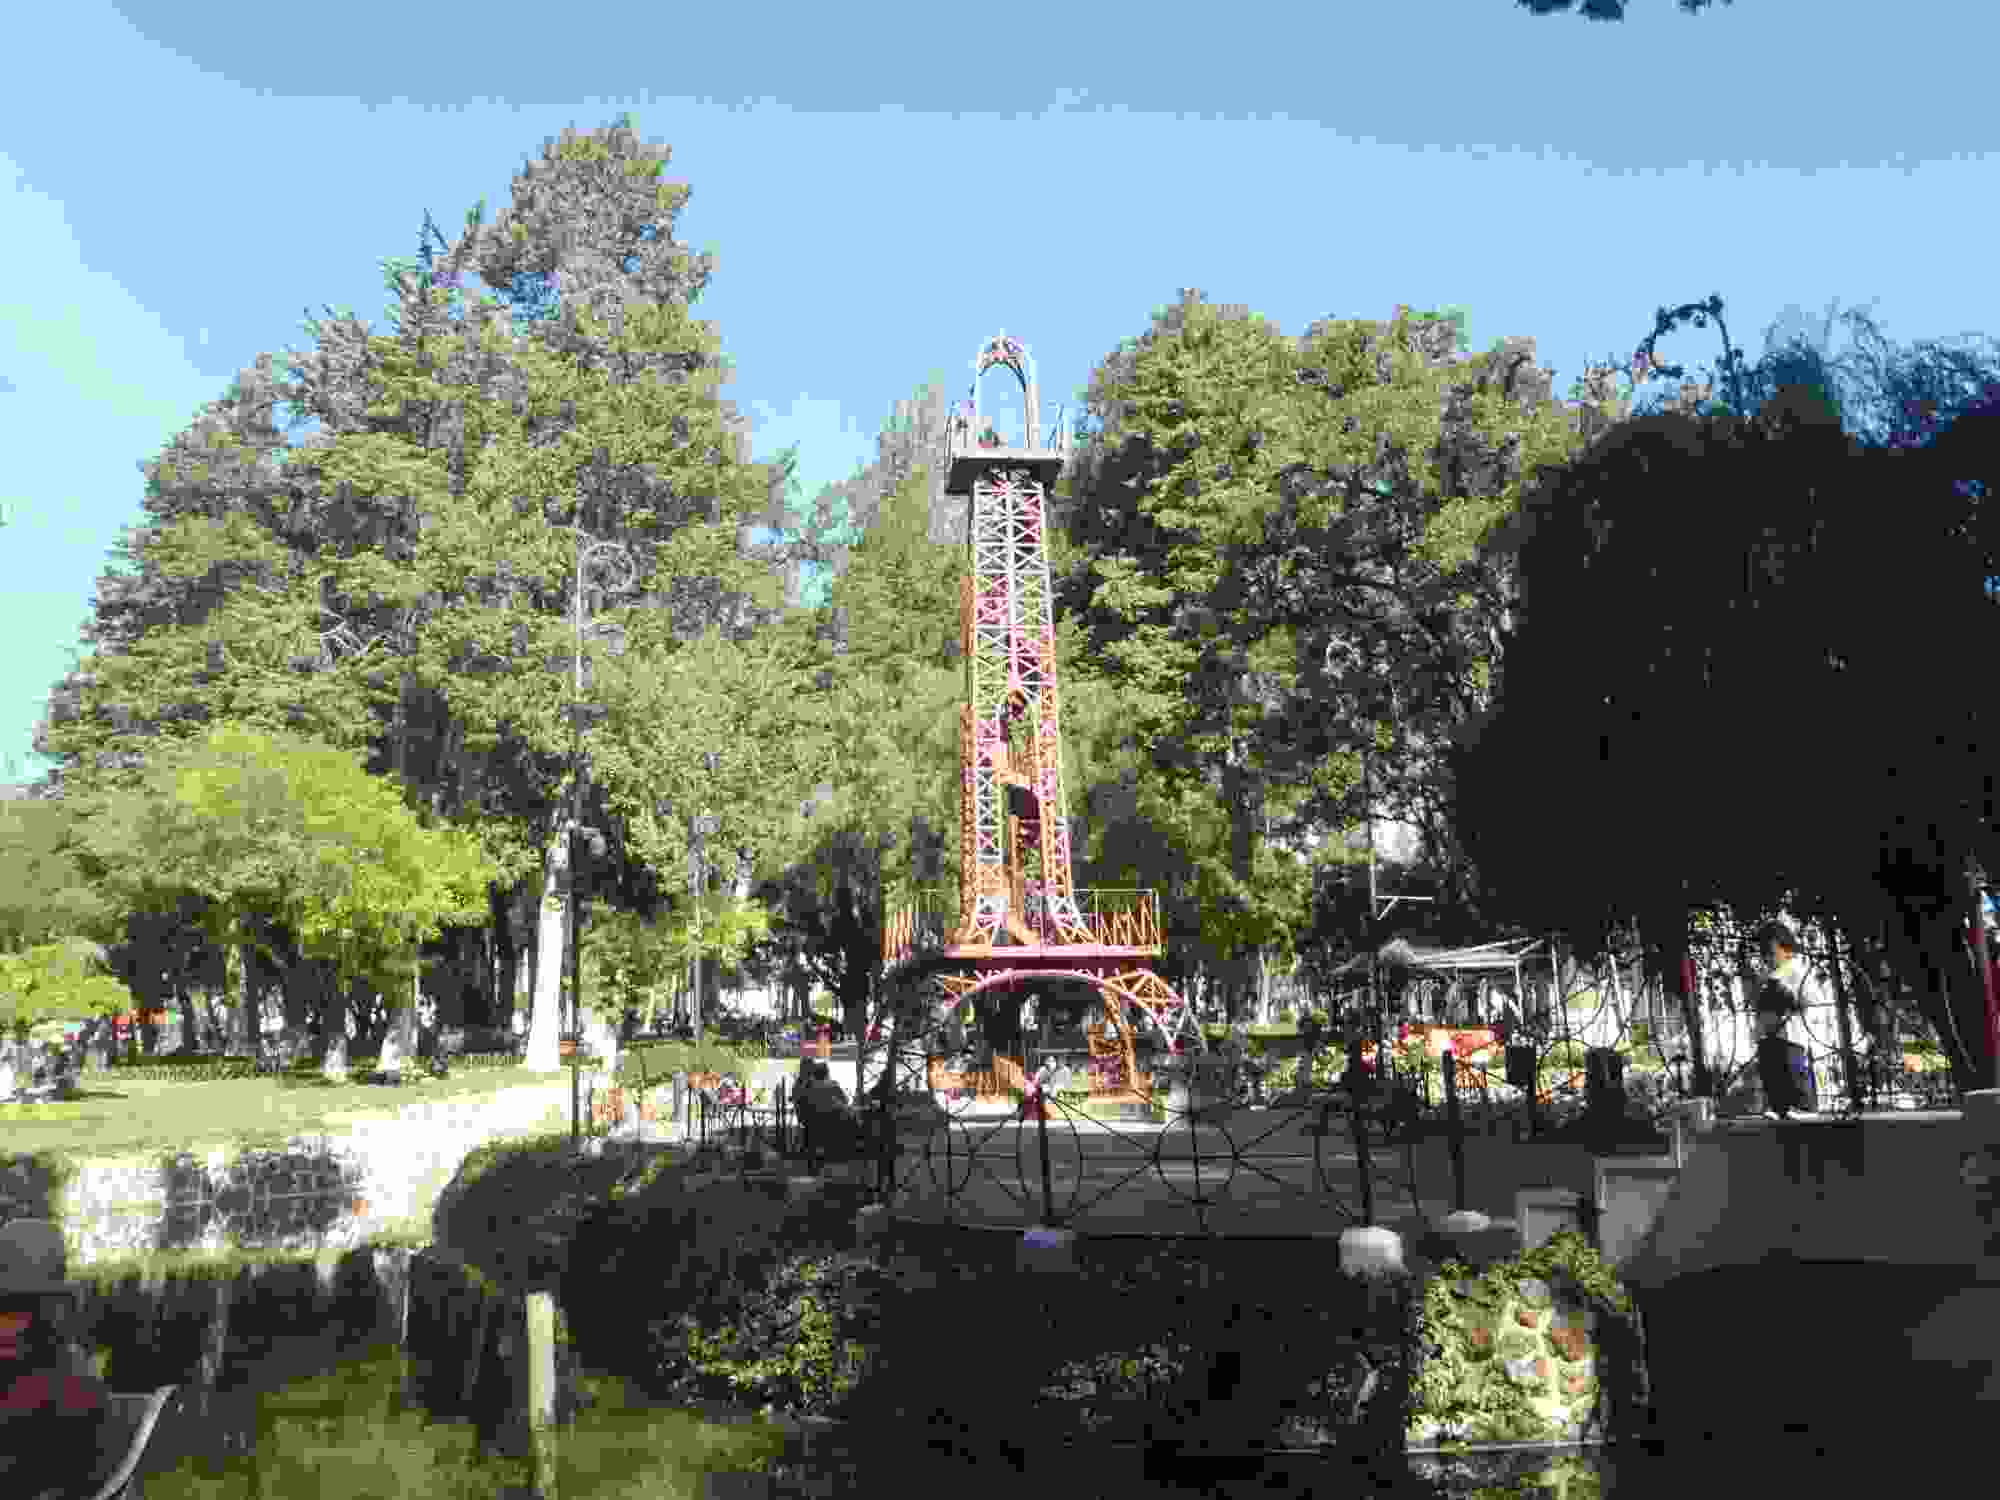
\includegraphics[width=\mywidth]{../wp-content/uploads/2015/04/wpid-wp-1429063685140.jpg} \end{center}

 Le Cementario General :
\begin{center} 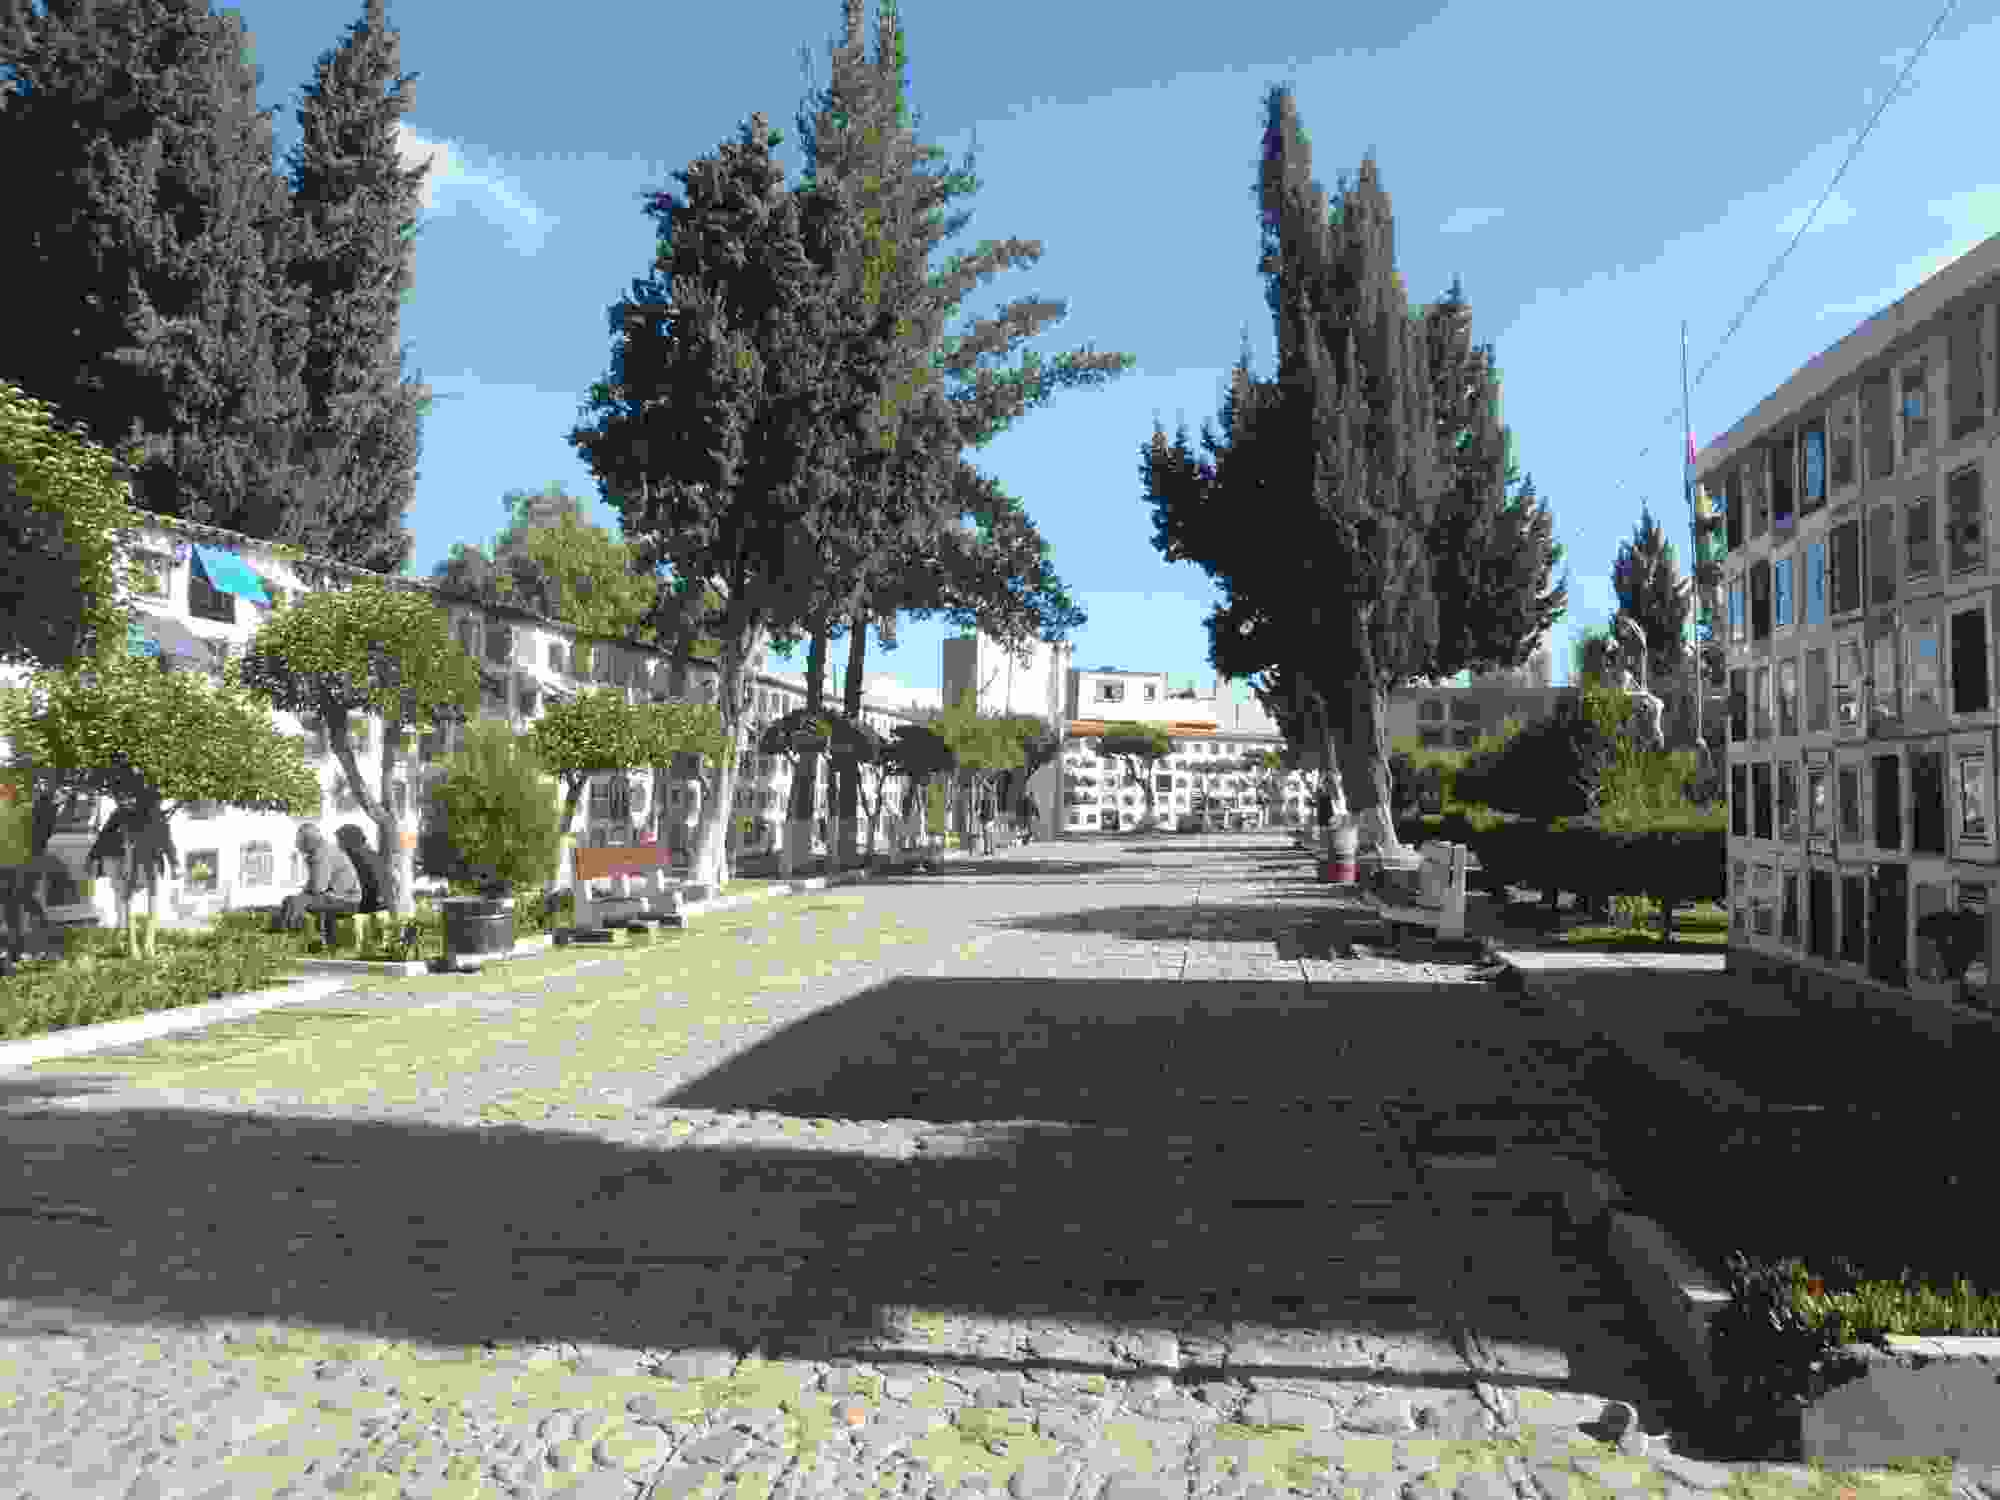
\includegraphics[width=\mywidth]{../wp-content/uploads/2015/04/wpid-wp-1429063755883.jpg} \end{center}
\begin{center} 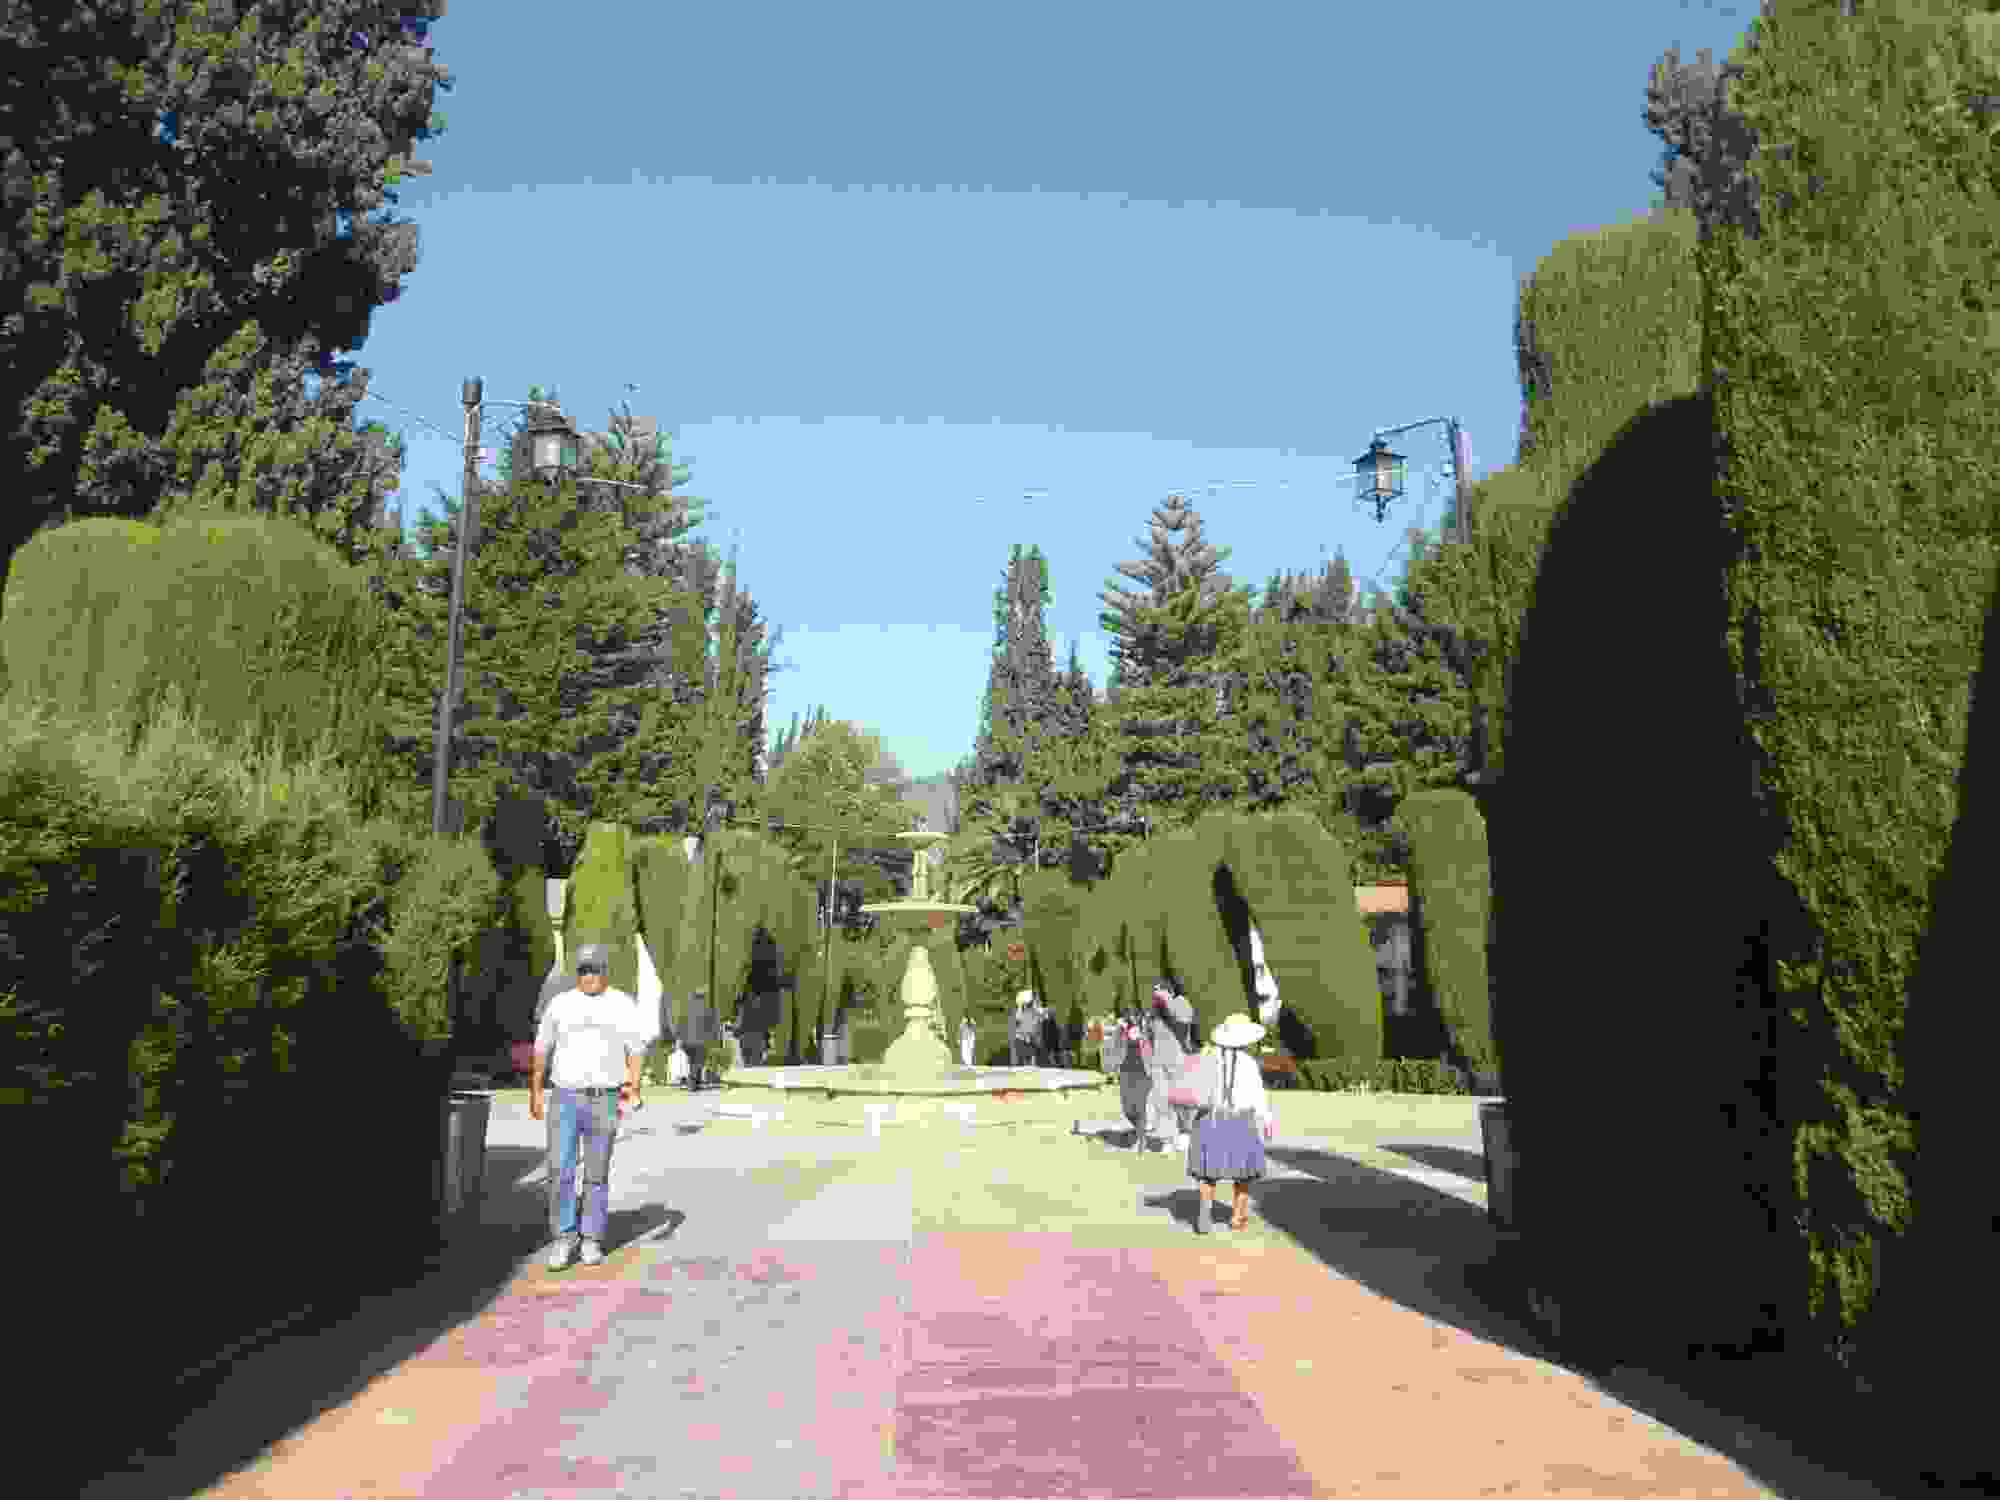
\includegraphics[width=\mywidth]{../wp-content/uploads/2015/04/wpid-wp-1429063782119.jpg} \end{center}

 Grâce à Couchsurfing j'ai rencontré Omar un étudiant bolivien. Avec 2 de ses amis, on a visité le parc des dinosaures :
\begin{center} 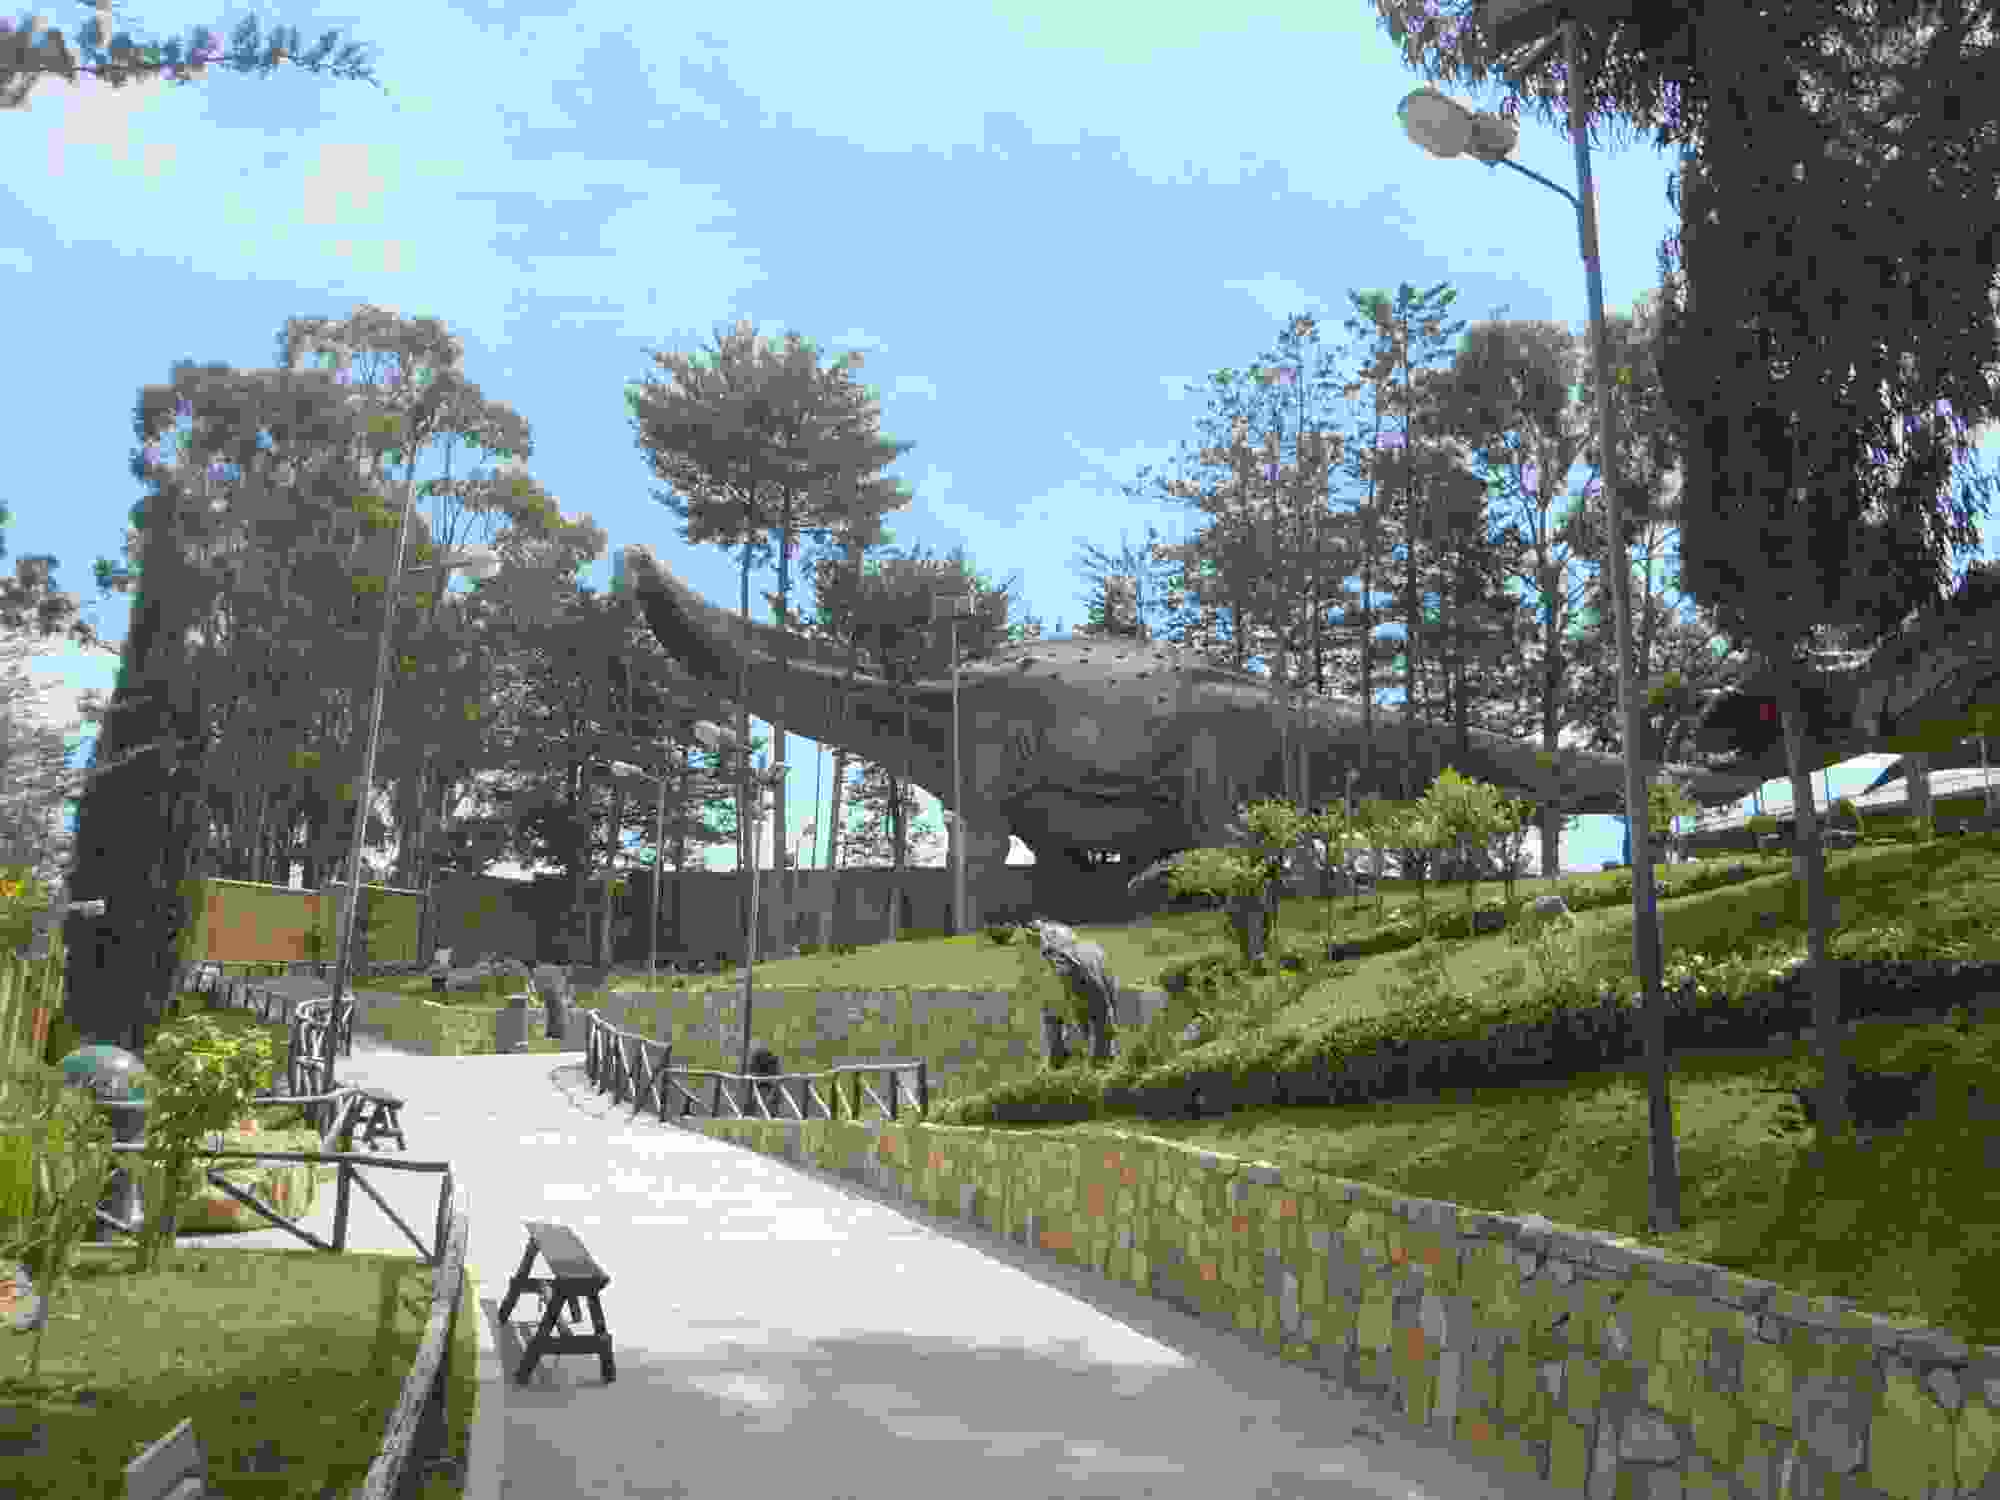
\includegraphics[width=\mywidth]{../wp-content/uploads/2015/04/wpid-wp-1429064168634.jpg} \end{center}
\begin{center} 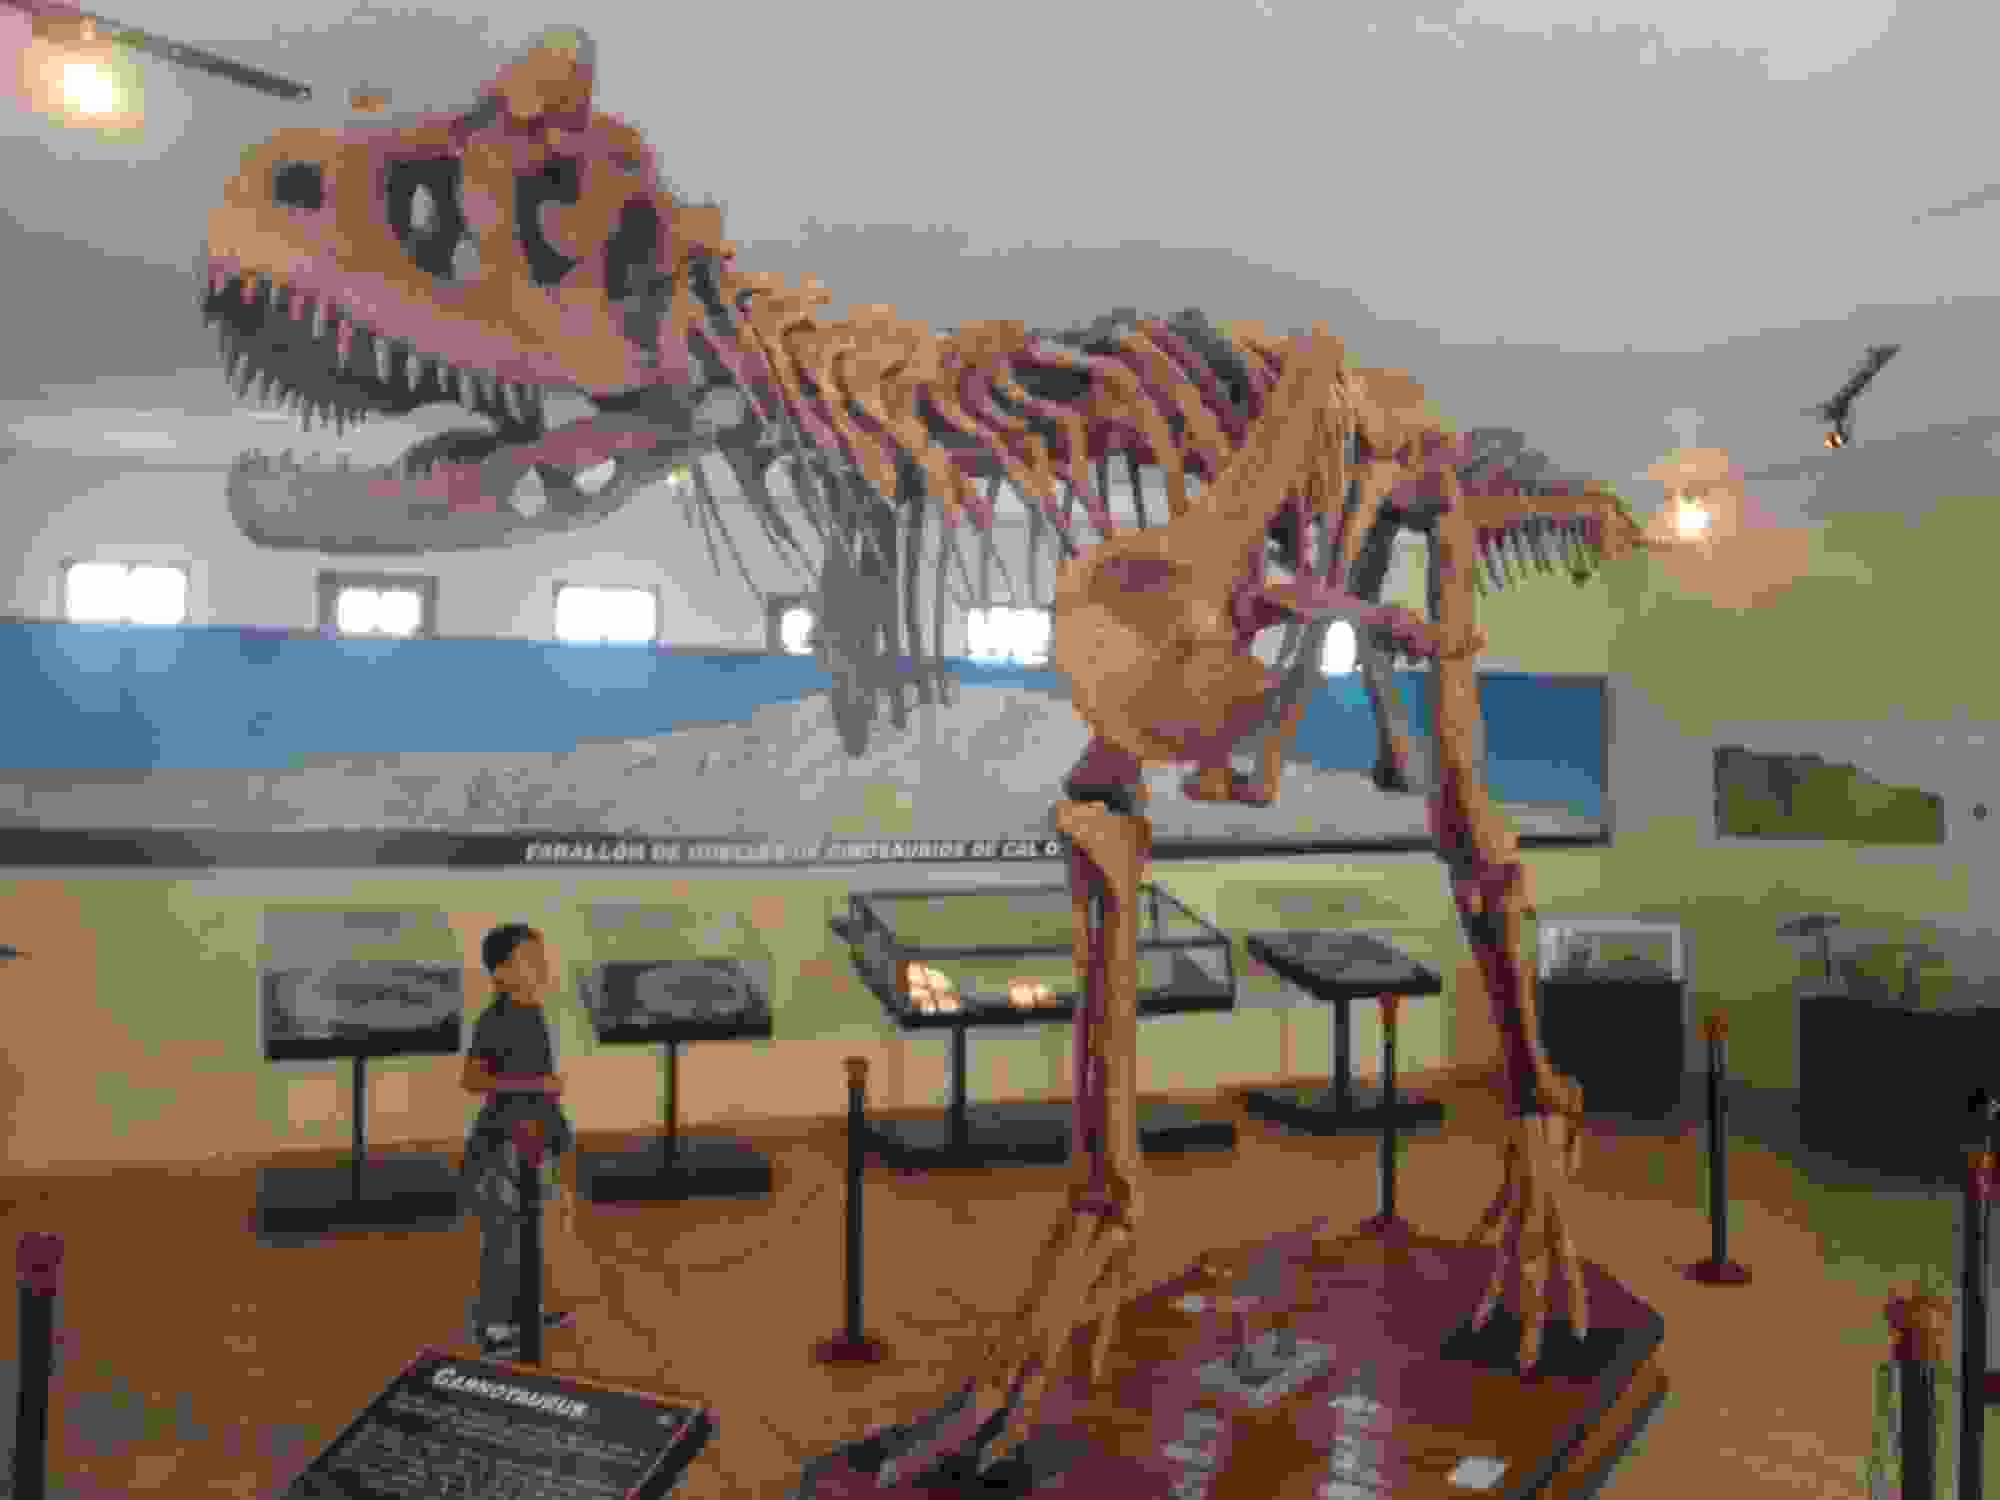
\includegraphics[width=\mywidth]{../wp-content/uploads/2015/04/wpid-wp-1429064265257.jpg} \end{center}

 La tectonique des plaques a fait passer cette immense falaise de l'horizontale à la verticale. Puis l'exploitation du site pour la fabrication de ciment a permis de découvrir des centaines d'empreintes de dinosaures. 
\begin{center} 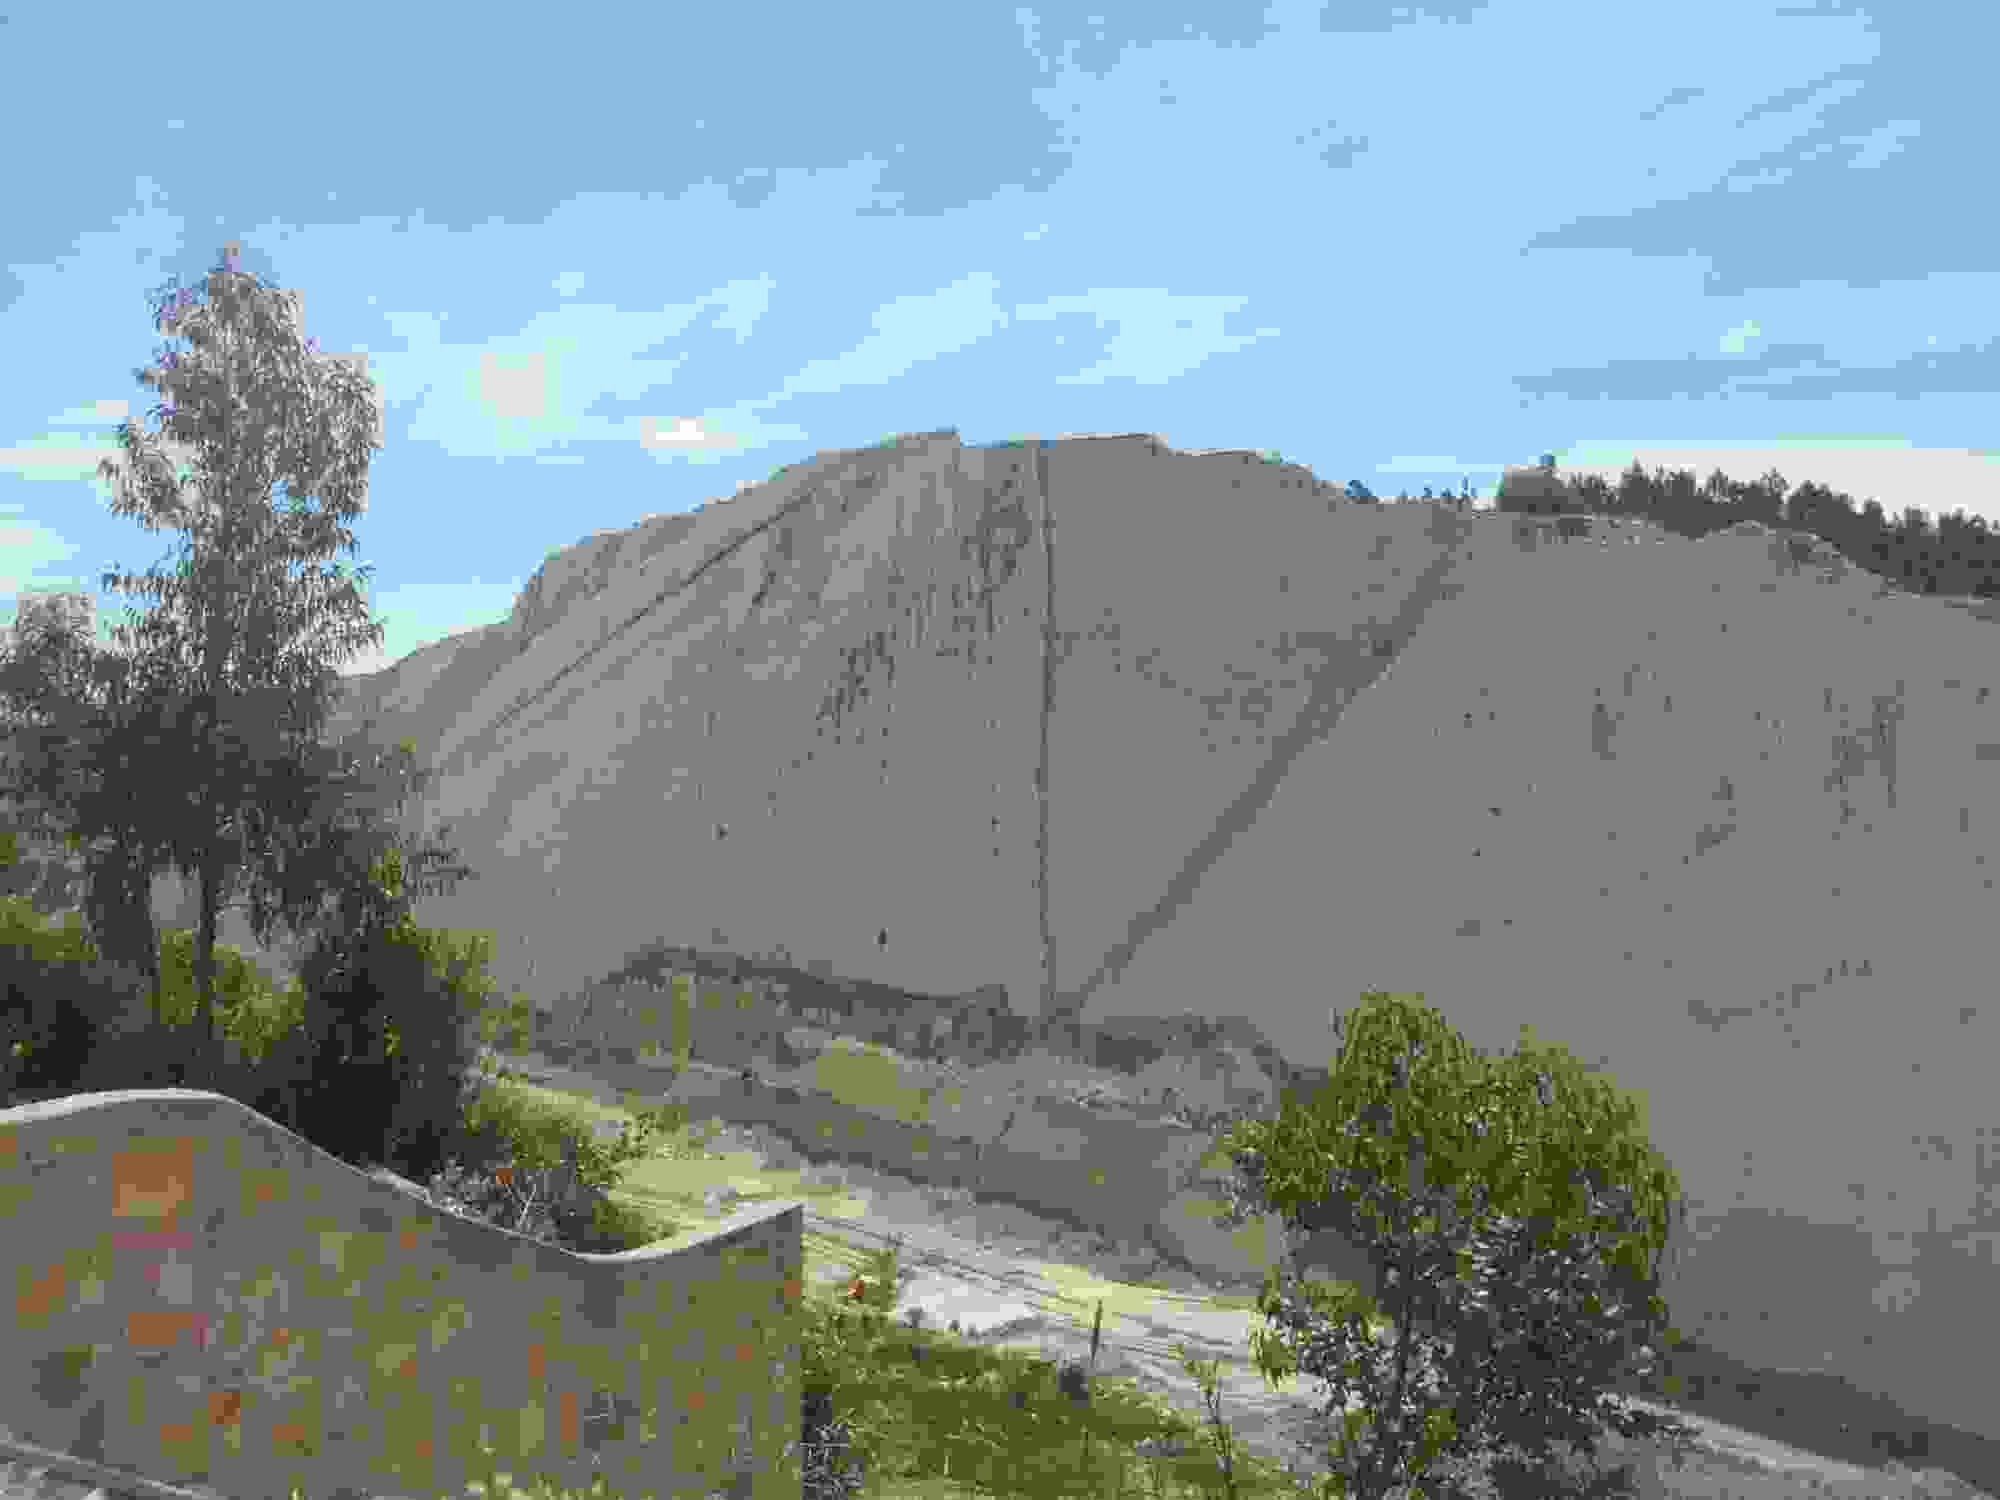
\includegraphics[width=\mywidth]{../wp-content/uploads/2015/04/wpid-wp-1429064563362.jpg} \end{center}
\begin{center} 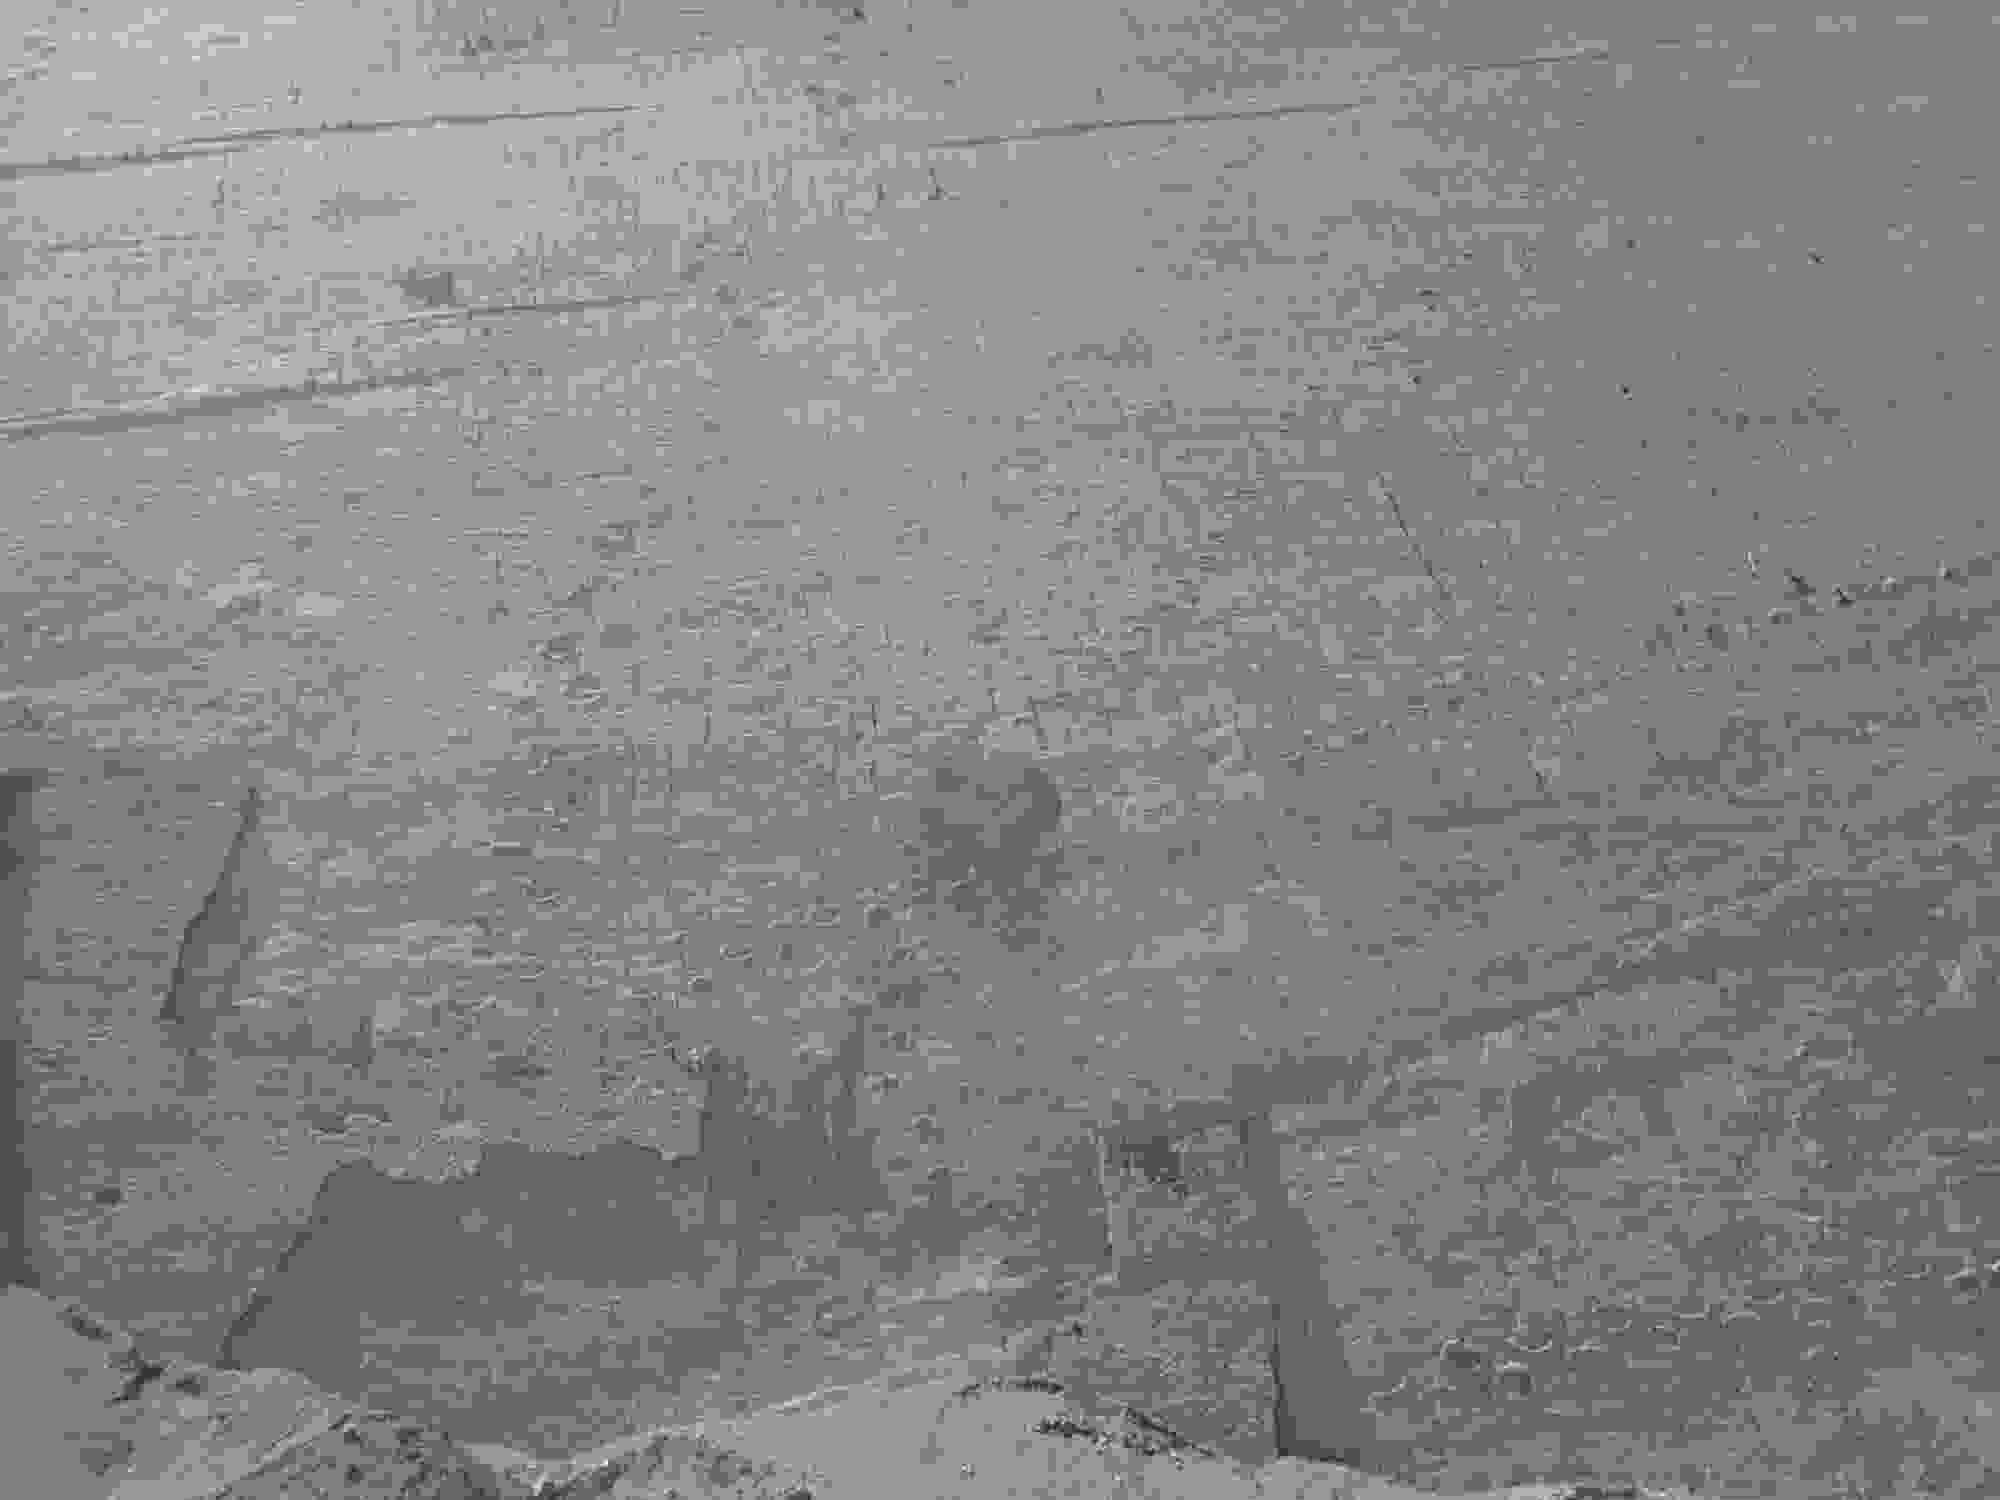
\includegraphics[width=\mywidth]{../wp-content/uploads/2015/04/wpid-wp-1429064631714.jpg} \end{center}
\begin{center} 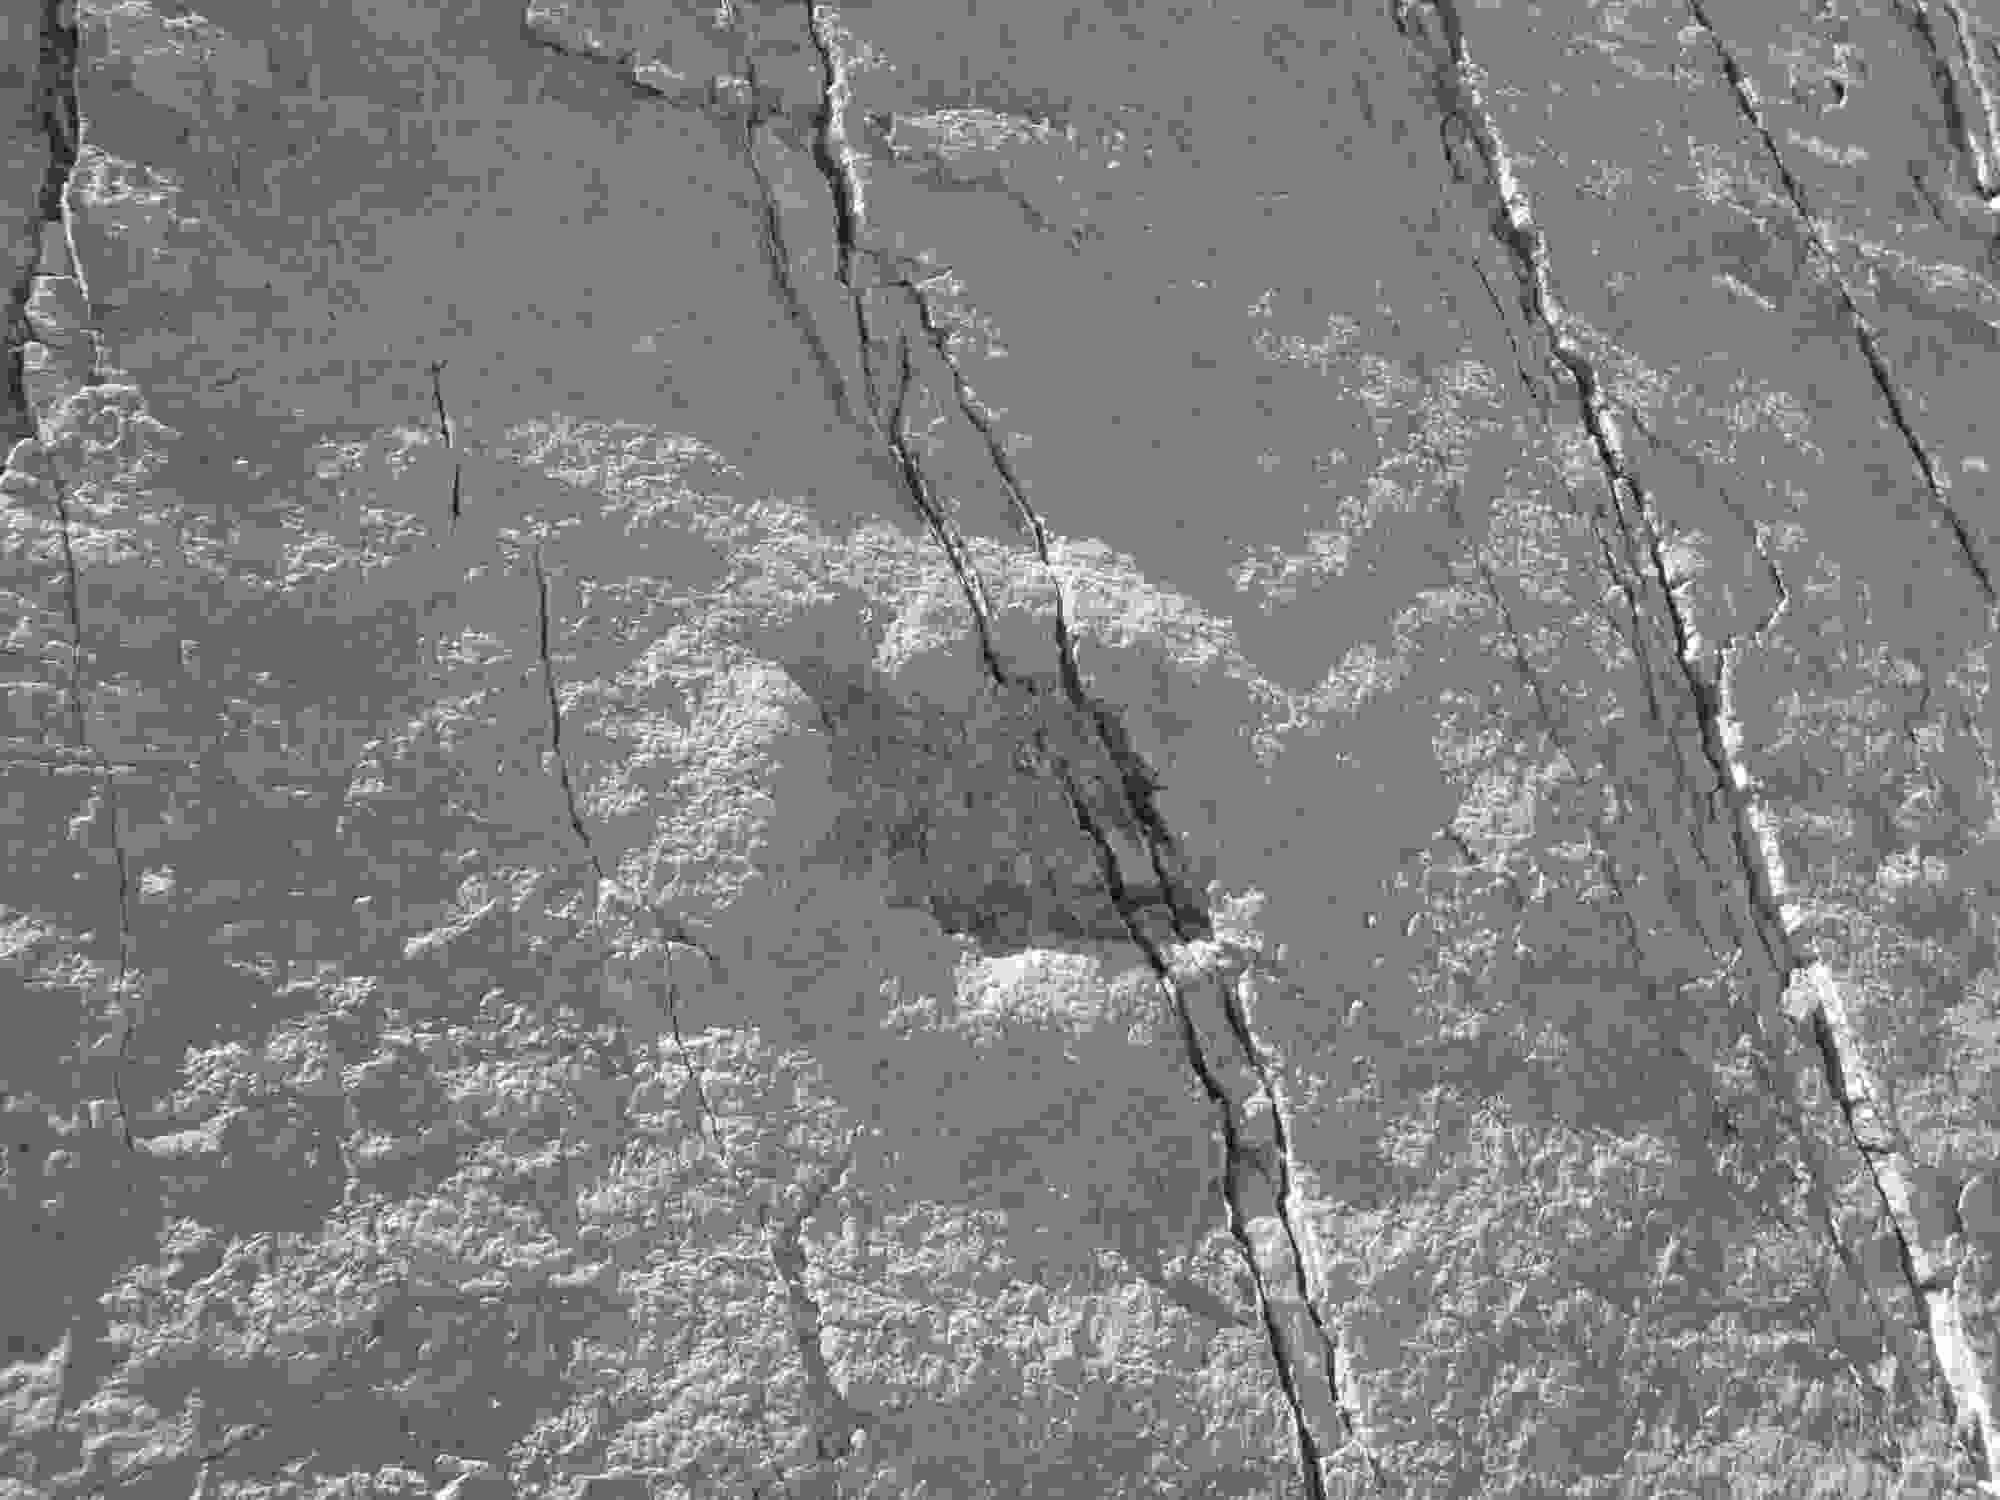
\includegraphics[width=\mywidth]{../wp-content/uploads/2015/04/wpid-wp-1429064717017.jpg} \end{center}
\begin{center} 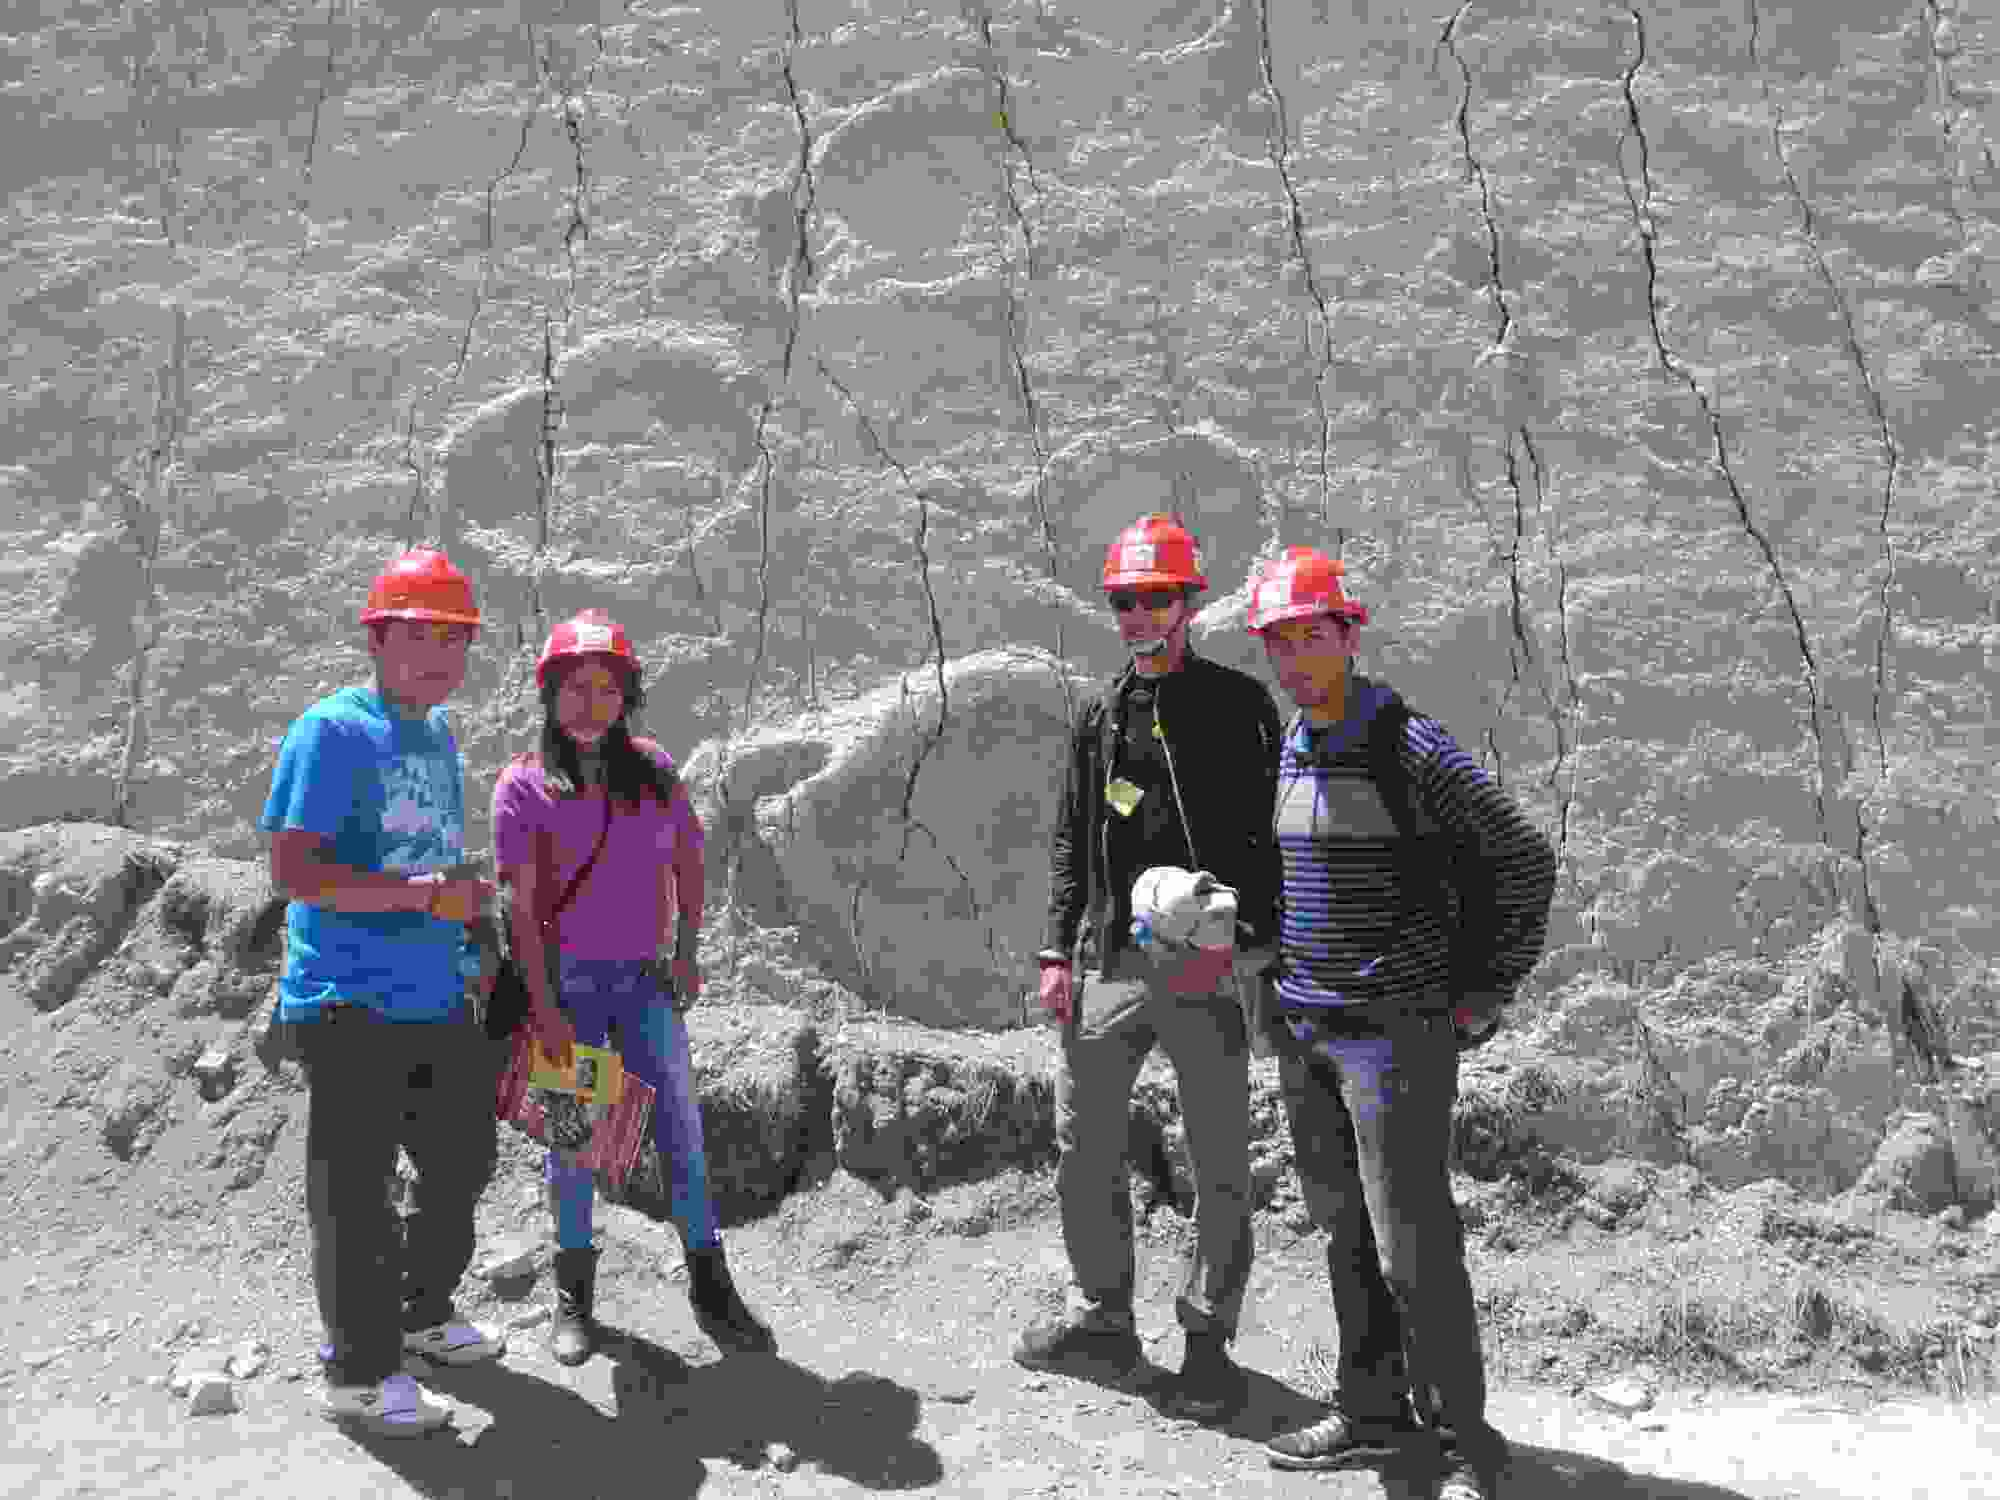
\includegraphics[width=\mywidth]{../wp-content/uploads/2015/04/wpid-wp-1429064728965.jpg} \end{center}